%\title{Template for a Thesis}
%%%%%%%%%%%%%%%%%%%%%%%%%%%%
% PREAMBLE OF THE DOCUMENT %
%%%%%%%%%%%%%%%%%%%%%%%%%%%%
%
%%%%%%%%%%%%%%%%%%%%%%%%%%%%%%%%%%%%%%%%%%%%%%%%%%%%%%%%%%%%%%%%
%
% 				         Edited by Nicola Rainiero
%				         http://rainnic.altervista.org/tag/latex
%			       	     ---------------------------------------
%%%%%%%%%%%%%%%%%%%%%%%%%%%%%%%%%%%%%%%%%%%%%%%%%%%%%%%%%%%%%%%%
%
% book - Default class for a normal book
\documentclass[a4paper,11pt,oneside,reqno,table]{book}


% extbook - a class for text bigger than 12pt
%\documentclass[a4paper,14pt,twoside,openright,reqno,table]{extbook}

% Options in detail:
% openany - allows chapter and similar openings to occur on left hand pages
% openright - allows chapter and similar openings to occur on right hand pages
% fleqn  - left-alignment of formulas
% leqno - labels formulas on the left-hand side instead of right
% reqno - labels formulas on the right-hand side
% draft - in draft mode the figures are not loaded, useful for speeding up typesetting
% onecolumn or twocolumn
% oneside (default for article and report)
% twoside (default for book)
% table  --> to avoid the message: package xcolor has already been loaded ...

\usepackage{packages}
\usepackage{my_listings}
% Almost all the settings are defined in packages.sty

% Put a grey textual watermark on document pages (PS mode only)
%\usepackage[italian,light,first,bottomafter]{draftcopy}

% Put a grey textual watermark on document pages (PDF mode)
%\usepackage{draftwatermark}
% If you want to change the default DRAFT text
%\SetWatermarkText{DRAFT}
% If you want to change the default grey color of the text
%\SetWatermarkColor{red}

%%%%%%%%%%%%%%%%%%%%%%%%%%%%%%%%%%%%%%%%%%%
%   DOCUMENT: an ordered list of files    %
%             that you can include or not %
%             in your document            %
%%%%%%%%%%%%%%%%%%%%%%%%%%%%%%%%%%%%%%%%%%%
\begin{document}

% FRONTISPIECE %
\begin{titlepage}
% \changepage with:
% {textheight}{textwidth}{evensidemargin}{oddsidemargin}{columnsep}
% {topmargin}{headheight}{headsep}{footskip}
\changepage{}{}{}{-7.5 mm}{}{}{}{}{}
%\InMiddlePage {copertina}

\begin{center}
%\includegraphics [width=.15\columnwidth, angle=0]{unipd1}\\ % height
{\LARGE \bf \scshape Universit\`a Politecnica delle Marche}\\
\vspace{0.2cm}
{\Large \bf \scshape Facolt\`a di Ingegneria}\\
\vspace{0.2cm}
{\Large Dipartimento di Ingegneria dell'Informazione}\\
\vspace{0.2cm}
{\large Corso di Laurea Magistrale in Ingegneria Informatica e dell'Automazione}\\

\rule{150mm}{.2mm}


\vspace{10mm}

\begin{figure}[h!]
	\centering
	
\includegraphics[width=3.5cm]{logo_univpm}
\end{figure}

\vspace{10mm}

\textbf{ \large \scshape Tesi di Laurea}

\vspace{8mm}

\Large{\bf Progettazione e implementazione di un sistema per il riconoscimento e il tracciamento di prodotti vitivinicoli di qualità}

\vspace{7mm}

\Large{\bf Design and implementation of a system for recognition and tracking of quality wine products}

\end{center} 	
\vspace{20mm} 	
\begin{center}
\begin{tabular}{lcl}
	{\large Relatore} & \ \hskip 6cm \ & {\large Candidato} \\
	\ & \ & \\
	{Prof. Domenico Ursino} \ & \ & {Compagnoni Paolo} \\
	\ & \ & \ \\
	\ & \ & \ \\
 {\large Correlatore} & \ \hskip 6cm \ & {} \\
	\ & \ & \\
	{Dott. Ferrante Marco} \ & \ & {} \\
	\ & \ & \ \\
	\ & \ & \ \\
	
\end{tabular}

\vspace{12mm}

\rule{150mm}{.2mm}

\textbf{\scshape Anno Accademico 2022-2023}
\end{center} 	
\end{titlepage}



%% FRONTMATTER %%
% The pages inside of frontmatter are in Roman numerals and the chapters will not have numeration
\frontmatter

% CREDITS %
\begin{titlepage}

\nonumber
\null \vspace {\stretch{1}}
	\begin{flushright}
%	\begin{verse}
\textit{Una nave in porto è al sicuro, \\
ma non è per questo che le navi sono state costruite} \\[5mm]
%	\end{verse}
	Benazir Bhutto
	\end{flushright}
\vspace{\stretch{2}}\null

\end{titlepage}
\cleardoublepage

% ABSTRACT %
%\selectlanguage{italian}
\begin{abstract}

In questi ultimi anni il tema dell'agricoltura di precisione ha assunto un'importanza sempre maggiore in quanto consente di ottimizzare la produzione dei prodotti alimentari e di prevedere le malattie che colpiscono le coltivazioni adottando misure preventive. Inoltre, il tracciamento dei prodotti è un'attività fondamentale che consente di effettuare delle campagne di richiamo di prodotti alimentari che risultano pericolosi per la salute. In questa tesi, è stato creato un prototipo di un'applicazione Android in grado di riconoscere, tramite fotocamera, le bottiglie di vino e mostrarne all'utente informazioni relative al vigneto di provenienza. In particolare, si è illustrato l'intero processo che va dalla creazione del modello tridimensionale fino allo sviluppo dell'applicazione in Unity. Successivamente sono stati effettuati dei confronti tra l'applicazione e i sistemi di tracciamento dei prodotti alimentari ed infine è stata effettuata una SWOT Analysis dei rischi individuati nel progetto.
\\[1cm]
\textbf{Keyword}: Agricoltura di precisione, Tracciamento dei prodotti, Data Analytics, Agricoltura 4.0, Ottimizzazione della produzione, Augmented Reality, Unity, Vuforia Engine
\end{abstract} 

\selectlanguage{italian}

% TOCs %
%% To help hyperref to jump to the correct page
\phantomsection
\addcontentsline{toc}{chapter}{Indice}
\tableofcontents
\clearpage

\tableofcontents   
\listoffigures

% GLOSSARY
%\cleardoublepage
% To help hyperref to jump to the correct page
\phantomsection
% To add the Glossary in the table of contents
\addcontentsline{toc}{chapter}{Glossario}
% Prints the glossary
\printglossary
% In order to update the glossary you have to execute:
% makeindex -s main.ist -t main.alg -o main.acr main.acn
% to insert an item in the document:
% \newglossaryentry{item_label}{name={item}, description={description}}
% if it doesn't appear you have to initialize it:
% \glsadd{item_label}
% or if it is called again in the following text:
% \gls{item_label}

% SYMBOLS %
%\cleardoublepage
% To help hyperref to jump to the correct page
\phantomsection
% To add the Index of Symbols in the table of contents
\addcontentsline{toc}{chapter}{Elenco dei simboli}
% Prints the Index of Symbols
\printglossary[type=\acronymtype,title=Elenco dei simboli]
% In order to update the symbols you have to execute:
% makeindex -s main.ist -t main.glg -o main.gls main.glo
% to insert an item in the document::
% \newacronym{item_label}{name={item}, description={description}}
% if it doesn't appear you have to initialize it:
% \glsadd{item_label}
% or if it is called again in the following text:
% \gls{item_label}

%% MAINMATTER %%
% The pages inside of mainmatter are in Arabic numerals and the chapters will have numeration
\mainmatter

%\part{Studio iniziale}
\phantomsection
\addcontentsline{toc}{chapter}{Introduzione}
\chapter*{Introduzione}
\markboth{Introduzione}{}

L'evoluzione tecnologica nel settore agricolo ha introdotto concetti fondamentali, come l'agricoltura di precisione e il tracciamento dei prodotti alimentari, rivoluzionando il modo in cui affrontiamo le sfide legate alla produzione agricola.

L'agricoltura di precisione, con la sua capacità di raccogliere dati dettagliati attraverso l'uso di tecnologie avanzate, ha dimostrato di essere una risorsa cruciale per ottimizzare le pratiche agricole. Il tracciamento dei prodotti alimentari, d'altro canto, ha assunto un ruolo di primaria importanza nella garanzia della qualità e nella sicurezza alimentare, permettendo ai consumatori di accedere a informazioni accurate riguardo all'origine e alla produzione degli alimenti che consumano.

Nel contesto specifico della viticoltura, la prevenzione delle malattie rappresenta una sfida fondamentale. La peronospora, una delle patologie più comuni, può causare gravi danni alle viti, influenzando la qualità e la quantità della produzione. In risposta a questa esigenza, l'obiettivo principale di questo progetto è sviluppare un sistema in grado di monitorare in tempo reale lo stato di salute del vigneto, utilizzando lo smartphone per riconoscere le bottiglie di vino, e fornire informazioni dettagliate sulle condizioni della coltivazione.

Attraverso l'integrazione di dati provenienti da sensori sul campo e l'utilizzo di dati provenienti dall'API OpenWeather, l'applicazione proposta mira non solo a identificare le bottiglie di vino, ma anche a fornire una panoramica sulle condizioni del vigneto consentendo interventi tempestivi per prevenire e gestire le malattie.

Il presente lavoro si propone, quindi, di contribuire allo sviluppo di soluzioni innovative nel settore vitivinicolo, sfruttando le potenzialità dell'agricoltura di precisione e del tracciamento avanzato per garantire la sostenibilità e la prosperità del settore, promuovendo al contempo una maggiore consapevolezza nei consumatori riguardo all'origine e alla qualità dei prodotti vinicoli.

Più specificatamente, ci si propone di sviluppare un'applicazione Android in grado di riconoscere le bottiglie di vino e visualizzarne le informazioni relative allo stato di salute del vigneto di provenienza. Inizialmente, sono stati identificati gli strumenti software necessari allo sviluppo dell'applicazione, tra cui \textit{Unity}, \textit{Vuforia Engine}, e \textit{Polycam}. Successivamente, sono stati illustrati gli aspetti progettuali, con la selezione delle versioni di ciascun software per evitare potenziali problemi di compatibilità. Sono stati presentati i Class Diagram e i Sequence Diagram al fine di fornire un quadro chiaro degli aspetti software cruciali dell'applicazione.

Nella fase successiva, è stato esaminato approfonditamente il codice delle classi C\# più rilevanti del progetto, al fine di chiarire ogni aspetto implementativo e giustificare le scelte progettuali effettuate durante la fase di progettazione.

L'ultima parte del lavoro si è concentrata sul confronto dell'applicazione con i sistemi di tracciamento dei prodotti alimentari, analizzando gli elementi in comune e non tra l'applicazione sviluppata e tali sistemi.

Successivamente, è stata condotta un'analisi SWOT accurata dell'applicazione. Infine, sono stati indicati possibili sviluppi futuri.

La tesi è composta da sette capitoli strutturati come di seguito specificato:
\begin{itemize}
	\item Nel Capitolo 1 sarà introdotto il mondo molto complesso dell'agricoltura di precisione partendo dalla sua storia per poi approfondire le tecnologie utilizzate oggi nel settore.
	\item Nel Capitolo 2 si presenterà il tema del tracciamento dei prodotti alimentari che è strettamente legato alla tematica dell'agricoltura di precisione.
	\item Nel Capitolo 3 verranno introdotti tutti gli strumenti software impiegati nello sviluppo dell'applicazione.
	\item Nel Capitolo 4 si concentrerà sugli aspetti progettuali del progetto, mostrando i Class Diagram e Sequence Diagram.
	\item Il Capitolo 5 è dedicato al lato implementativo del progetto, descrivendo il codice impiegato nello sviluppo dell'applicazione Android.
	\item Nel Capitolo 6 si effettuerà un confronto dell'applicazione con i sistemi di tracciamento dei prodotti alimentari.
	\item Nel Capitolo 7 si effettuerà una discussione del progetto in merito all'analisi dei principali rischi individuati.	
	\item Infine, si trarranno le conclusioni in merito al lavoro svolto e si delineeranno alcuni possibili sviluppi futuri.
\end{itemize}

\chapter{L'agricoltura di precisione}

\begin{preamble}
{\em Nel primo capitolo, si introduce il concetto di agricoltura di precisione, fornendo inizialmente una breve definizione. Successivamente, si esplorerà il percorso storico che condurrà dalle origini dell'agricoltura fino ai giorni nostri, dove l'agricoltura di precisione è diventata una pratica diffusa. Questo  permetterà di comprendere l'evoluzione della ricerca in questo campo fino all'attuale stato dell'arte.

In seguito, si esamineranno le due tecnologie fondamentali su cui si basa l'agricoltura di precisione: il machine learning e il deep learning. Per entrambe queste tecnologie, si presenterà in modo conciso le tecniche più utilizzate, sia in generale che nel contesto specifico dell'agricoltura di precisione, mettendone in luce vantaggi e svantaggi.

Infine, nell'ultima sezione, affronteremo il tema dell'Internet delle cose (IoT), che rappresenta il contesto in cui si colloca l'applicazione sviluppata in Unity.
}
\end{preamble}

\section{Introduzione all'agricoltura di precisione}

L'agricoltura di precisione può essere definita come un approccio integrato all'agricoltura che impiega dati geo-referenziati, tecnologie digitali, sensori, automazione e analisi avanzate per monitorare, gestire e ottimizzare con precisione ogni aspetto del processo agricolo, dalla preparazione del suolo alla coltivazione, dalla raccolta alla distribuzione. 

L'obiettivo principale è massimizzare l'efficienza nell'uso delle risorse, minimizzare gli impatti ambientali, migliorare la produttività e la qualità delle colture, e garantire una gestione sostenibile delle aziende agricole. L'agricoltura di precisione si basa su un approccio personalizzato, in cui le decisioni vengono prese in tempo reale in base alle specifiche condizioni e necessità di ogni singola area coltivata, consentendo agli agricoltori di ottimizzare i rendimenti e la redditività, riducendo, al contempo, gli sprechi e l'impatto ambientale.

\section{Storia dell'agricoltura di precisione}

Gli antichi, pur comprendendo le differenze nella produzione agricola tra i vari campi, sembravano dare scarsa importanza alle variazioni all'interno di ciascun campo, come testimonia Catone nel 160 a.C. 

I Romani valutavano l'acquisto di terra principalmente in base alla loro impressione generale sulla gestione della fattoria, la sua posizione nel paesaggio e le caratteristiche del suolo. Per fertilizzare i campi, utilizzavano una serie di metodi tra cui concimi organici, compost e il liquido residuo dall'estrazione dell'olio d'oliva. Tuttavia, a causa del pesante carico di lavoro richiesto per le pratiche agricole fondamentali, sembra che abbiano dato scarsa attenzione alla variazione all'interno dei singoli campi. I proprietari terrieri si concentravano di più sulla gestione degli schiavi o dei liberti che sulla differenziazione dei terreni. Inoltre, l'acquisizione di nuove terre era spesso più prioritaria della gestione delle aree degradate all'interno dei campi. 

Nei secoli successivi, gli scienziati iniziarono a definire gli obiettivi della scuola agraria. Il primo tema sperimentale che emerse fu la necessità di affrontare la variabilità nella resa delle colture dovuta all'eterogeneità dei suoli. Nonostante gli sforzi per individuare aree il più omogenee possibile per condurre esperimenti sul campo, l'ostacolo dell'eterogeneità del terreno continuava a sfidare i ricercatori. 

Negli anni venti del secolo scorso, si compirono notevoli progressi per migliorare le decisioni legate alla variabilità spaziale su piccola scala. Robert A. Fisher iniziò un lavoro rivoluzionario presso la Rothamsted Experiment Station di Harpenden, in Inghilterra, nel 1919. In sette anni, sviluppò una serie di strumenti statistici che sarebbero diventati la base per la maggior parte degli esperimenti su piccole aree, e persino interi campi. L'applicazione dei principi enunciati da Fisher e l'ampliamento degli strumenti statistici per affrontare le sfide legate alle pendenze e alle differenze sistematiche nei terreni, si rivelarono fondamentali per mitigare l'impatto della variabilità spaziale negli esperimenti su piccole aree condotti da generazioni di ricercatori sul campo. Tuttavia, nessuno di questi strumenti si è dimostrato particolarmente idoneo a gestire la variabilità nei fattori quali nutrienti, infestazioni da erbe infestanti, presenza di insetti, dosaggi di semina o altri input gestionali nei campi.

A partire dal 1920, gran parte dell'attenzione nell'agricoltura orientata alla specificità del suolo si è concentrata sulla gestione dei nutrienti per le coltivazioni. L'analisi del terreno è emersa come un aspetto cruciale, poiché è stata riconosciuta come un mezzo per valutare la capacità del suolo di fornire nutrienti, un concetto che risale ai lavori di Sprengel nel 1839. 

Nella procedura di analisi del terreno, un campione di suolo viene prelevato dal campo per poi essere sottoposto ad un trattamento per rimuovere detriti e piccoli sassi. Successivamente, il campione viene mescolato con un estrattore liquido, filtrato e il contenuto del nutriente di interesse viene quantificato per consentire un confronto con una quantità standard correlata a una potenziale risposta della coltura. Questa risposta può risultare vantaggiosa per la coltivazione o, in alcuni casi, avere effetti tossici, a seconda del tipo di elemento o composto estratto e della sua quantità nel terreno. 

La prima raccomandazione conosciuta per il campionamento del suolo al fine di gestire la variabilità nei campi agricoli fu pubblicata da Linsley e Bauer nel 1929. Questa raccomandazione suggeriva agli agricoltori di prelevare campioni di suolo a una profondità di 15 cm e analizzarli seguendo una griglia di 0,4 ettari, con ulteriori prelievi a 30 cm di profondità. La motivazione dietro questa pratica era legata alla difficoltà di diffondere il calcare agricolo in campi con terreno acido.

Nel 1938, gli agricoltori avevano ormai a disposizione numerose macchine per l'applicazione di fertilizzanti, molte delle quali venivano utilizzate regolarmente, comprese quelle per la distribuzione, la localizzazione in collina e l'applicazione vicino ai semi.

Dal decennio degli anni '50 fino ai giorni nostri, il campionamento base del suolo è stato principalmente rappresentato da campioni compositi che rappresentano un intero campo. Nonostante i ricercatori esperti nella variazione spaziale dei nutrienti delle colture abbiano consigliato di includere solo terreni relativamente omogenei e simili in un campione composito, essi venivano prelevati da diverse zone all'interno dei campi, delimitate dai confini imposti dagli agricoltori, considerando la variabilità dei suoli al loro interno. 

Negli anni '60, si verificarono anche importanti avanzamenti nell'affrontare direttamente la variabilità spaziale dei nutrienti del suolo, con l'introduzione del campo statistico della geo-statistica da parte di un ricercatore canadese di nome Matheron nel 1963.

Poiché il campionamento del suolo o di qualsiasi altra entità all'interno di un campo agricolo identifica soltanto la piccola area da cui vengono prelevati campioni, piante, parti di piante o misurazioni, la stragrande maggioranza delle zone all'interno del campo rimane sconosciuta rispetto ai valori osservati. Di conseguenza, è necessario stimare o \textit{interpolare} i valori delle aree non campionate nel campo per prendere decisioni basate sui risultati del campionamento. Il \textit{Kriging} è il metodo preferito per raggiungere questo obiettivo, sebbene richieda un insieme minimo di almeno 30 osservazioni per essere applicato con successo.

Negli anni '80, il Dipartimento della Difesa degli Stati Uniti ottenne finanziamenti dal Congresso per sviluppare il sistema di posizionamento satellitare noto come \textit{GPS}. La rete GPS era composta da 24 satelliti e fu completata nel 1994. L'anno precedente, nel 1993, venne siglato un accordo tra il Dipartimento della Difesa e il Dipartimento dei Trasporti, che consentì l'utilizzo civile del sistema GPS. Questa apertura del GPS al settore agricolo rappresentò una svolta fondamentale per l'agricoltura di precisione, e in breve tempo diverse aziende iniziarono a offrire sistemi GPS per l'agricoltura.

Inizialmente, i sistemi GPS originali avevano una precisione che non permetteva la localizzazione entro pochi metri dalla posizione desiderata. Tuttavia, le aziende agricole e gli agricoltori risolsero questo problema installando torri di correzione cinetica in tempo reale, che migliorarono notevolmente la precisione del posizionamento. Va notato che i segnali GPS provenienti direttamente dai satelliti potevano presentare errori dovuti alle condizioni atmosferiche. Per affrontare questi errori, vennero sviluppati ricevitori e trasmettitori differenziali satellitari correttivi, come quelli adottati nel sistema \textit{GreenStar} di John Deere.

La determinazione della topografia può presentare un impatto significativo sullo sviluppo del suolo e sul movimento dell'acqua all'interno del terreno, influenzando così la produttività delle coltivazioni. La misurazione dell'elevazione può essere effettuata con il GPS differenziale dal quale è possibile ottenere non solo la latitudine e la longitudine, ma anche l'altitudine della posizione GPS.

Un approccio innovativo al rilevamento topografico è stato introdotto con lo sviluppo del \textit{LiDAR (Light Detecting And Ranging)}. Il LiDAR ha visto la luce poco dopo l'invenzione del laser, agli inizi degli anni '60.

Oltre alla topografia, diversi altri strumenti sono stati impiegati nello sviluppo delle zone di gestione dei nutrienti. Tra questi strumenti, le immagini satellitari hanno svolto un ruolo cruciale, soprattutto per quanto riguarda la gestione dell'azoto. Con il tempo, le immagini satellitari si sono rivelate strumenti preziosi per delimitare le zone di gestione dell'azoto durante la stagione agricola, integrando dati ottenuti tramite campionamento del suolo e altri metodi. Successivamente, sono stati sviluppati sensori basati sulle proprietà di trasmittanza elettrica del suolo ampiamente utilizzati per la delineazione delle zone di gestione dei nutrienti.

La conducibilità elettrica è stata anche direttamente correlata ai livelli di nitrato nel suolo in terreni che altrimenti sembravano uniformi. Inoltre, sia la conducibilità elettrica che il magnetismo possono essere utilizzati per rilevare differenze nella capacità di ritenzione dell'acqua, nei contenuti idrici del suolo, nella capacità di scambio cationico, nella porosità, nella salinità e nei gradienti di temperatura.
Tuttavia, in molti campi più di un fattore varia in modo indipendente dagli altri. In campi \textit{multivariabili}, i sensori di conducibilità elettrica e di flusso magnetico sono strumenti efficaci per identificare pattern e suddividere le zone, spesso superando altre tecniche.

La costruzione di algoritmi finalizzati all'applicazione dell'azoto durante la stagione si basa sulla previsione delle rese da parte del sensore in una striscia di azoto, confrontata con altre aree all'interno del campo. Il risultato di questo lavoro è stata la commercializzazione del sensore attivo-ottico \textit{GreenSeeker} nel 2002. Questo applicatore aveva la capacità di operare alle velocità del trattore nel campo e applicare l'azoto a ogni metro quadro di coltura in modo indipendente grazie alla sua serie di sensori e gruppi di ugelli posizionati ad ogni metro di larghezza della barra di spruzzatura.

La commercializzazione di successo dei sensori del suolo correlati ai nutrienti include il sensore del pH del suolo Veris Technologies. In uno studio, l'uso del sensore di pH Veris ha correlato il pH mappato dal sensore con i veri modelli di pH del terreno rispetto alle tecniche standard di campionamento del suolo site-specific, riducendo gli errori nelle raccomandazioni di dosaggio della calce del 50\%. Veris commercializza anche l'\textit{Optic Mapper}, che utilizza un rilevatore di infrarossi vicino all'interno del suolo per stimare il contenuto di materia organica di quest'ultimo.

\section{Machine Learning e Deep Learning nell’agricoltura di precisione}
\subsection{Introduzione}

L'agricoltura costituisce il pilastro fondamentale della nostra economia in quanto la crescente domanda di prodotti alimentari, derivante dall'incremento della popolazione, continua a crescere in modo costante. Per rispondere efficacemente a questa esigenza, il settore agricolo deve compiere notevoli progressi, ad esempio nell'effettuare calcoli precisi sulla produzione, sfruttando le attrezzature agricole più avanzate e aggiornate disponibili sul mercato. L'obiettivo principale di tali progressi è quello di soddisfare la crescente richiesta di coltivazioni alimentari di alta qualità.

Per avviare il processo verso l'agricoltura di precisione, si compiono passi iniziali fondamentali tra cui la previsione meteorologica e la valutazione degli effetti dei vari fertilizzanti, sfruttando il telerilevamento e i sensori per monitorare lo stato di salute delle colture.

Un importante passo avanti nell'evoluzione dell'agribusiness è consistito nell'introduzione dei sensori wireless nell'agricoltura e nell'industria alimentare. Questa innovazione ha aperto nuove possibilità nel monitoraggio e nell'ottimizzazione delle attività agricole e industriali legate al settore alimentare, contribuendo, così, a migliorare l'efficienza e la qualità della produzione agroalimentare.

Il concetto di gestione agricola si basa sulla raccolta di dati mediante osservazioni e misurazioni, nonché sulla capacità di rispondere in modo mirato alla variabilità delle colture sia tra i diversi campi che all'interno dello stesso campo. Questo approccio consente di ottimizzare la produzione agricola, ridurre gli impatti negativi sull'ambiente e garantire una fornitura continua di alimenti di alta qualità, contribuendo, così, a soddisfare le crescenti esigenze alimentari globali in modo sostenibile.

Affrontare questi problemi richiede un approccio integrato che coinvolga la ricerca scientifica, la formazione degli agricoltori, la promozione di pratiche agricole sostenibili e l'implementazione di regolamenti sanitari e ambientali rigorosi. Solo attraverso un impegno globale e coordinato è possibile affrontare efficacemente queste sfide e garantire una produzione agricola sicura, sostenibile e in grado di rispondere alle crescenti esigenze alimentari della popolazione mondiale.

L'agricoltura moderna affronta la sfida di mantenere l'equilibrio nell'ecosistema, evitando l'accumulo eccessivo di sostanze chimiche che possono danneggiare l'ambiente. La soluzione a questi problemi non può essere standardizzata poiché variano in base alle specifiche condizioni e alle manifestazioni locali. Per affrontare queste sfide complesse, è necessario adottare un approccio ecologico completo e flessibile, basato sull'osservazione e sull'analisi continua di tutti gli aspetti del sistema agricolo.

Un'opzione per mitigare questa situazione consiste nell'utilizzo dell'Intelligenza Artificiale, in particolare il Machine Learning. Quest'ultimo può fornire agli agricoltori dati e informazioni preziose per ottimizzare la produzione di colture, ridurre i costi iniziali e gestire le perdite dovute a calamità naturali. Questo approccio intelligente può contribuire a rendere l'agricoltura più efficiente ed ecologicamente sostenibile.

Un esempio di questo concetto è stato esplorato da Gomes e Leta nel 2012, che hanno studiato l'applicazione di tecniche informatiche nel settore agricolo e alimentare per migliorare la qualità dei prodotti. Allo stesso modo, Davies nel 2009 ha esaminato l'uso della visione artificiale e delle sue applicazioni nel settore agroalimentare. Queste ricerche dimostrano l'innovazione tecnologica, come quella apportata dall'Intelligenza Artificiale, possa portare a miglioramenti significativi all'agricoltura moderna.

\subsection{Il Machine Learning}

L'apprendimento automatico è un campo interdisciplinare che fonde l'informatica e la statistica, ponendosi come obiettivo l'analisi e la classificazione dei dati, svolgendo compiti che in genere richiederebbero l'intervento umano. Per raggiungere questo obiettivo, è necessario istruire i calcolatori in modo da risolvere problemi del mondo reale con la massima precisione possibile.

Di seguito, verranno illustrate le tre principali modalità di apprendimento automatico utilizzate negli algoritmi di Machine Learning, ovvero:

\begin{itemize}
    \item Supervised Learning;
    \item Unsupervised Learning;
    \item Reinforcement Learning ;
\end{itemize}

\subsubsection{Supervised Learning}

L'apprendimento supervisionato, o \textit{supervised learning}, come suggerisce il nome, richiede la guida di un supervisore per eseguire il compito. In questo tipo di apprendimento, una macchina viene addestrata utilizzando dati precedentemente raccolti e annotati, chiamati \textit{dati etichettati}. Questi dati consentono all'algoritmo di apprendimento supervisionato di analizzare il set di addestramento e produrre risultati corretti basati sulle etichette fornite. 

L'apprendimento supervisionato si suddivide in due categorie principali: la \textit{regressione} e la \textit{classificazione}. La regressione è una tecnica utilizzata per stabilire la relazione tra variabili indipendenti e variabili dipendenti, consentendo di predire valori numerici. D'altra parte, la classificazione consiste nel suddividere i dati in classi specifiche e distinte, assegnando un'etichetta a ciascuna classe.

L'approccio supervisionato è ampiamente utilizzato in applicazioni in cui è fondamentale effettuare previsioni o assegnare classificazioni basate su dati storici conosciuti e risultati noti, come nel riconoscimento delle immagini, nell'analisi del testo, nella diagnosi medica e in molte altre sfide decisionali.

\subsubsection{Unsupervised Learning}

L'apprendimento automatico non supervisionato, o \textit{unsupervised learning}, è un tipo di approccio in cui il modello non richiede una guida esterna, ma estrae informazioni dai dati stessi, principalmente da dati non etichettati. Gli algoritmi di apprendimento non supervisionato sono spesso utilizzati in compiti complessi e possono generare risultati eccellenti, in particolare quando si tratta di scoprire modelli nascosti nei dati. Gli algoritmi di apprendimento non supervisionato sono impiegati per scoprire pattern, cluster o associazioni all'interno dei dati in modo autonomo.

Questo tipo di apprendimento è stato applicato anche nell'agricoltura di precisione, dimostrando la sua utilità nell'analisi dei dati agricoli complessi. In generale, l'apprendimento non supervisionato può essere suddiviso in due categorie principali, ovvero il \textit{clustering} (raggruppamento di dati simili) e l'\textit{associazione} (individuazione di relazioni tra variabili o elementi nei dati).

\subsubsection{Reinforcement Learning}

Nell'apprendimento per rinforzo, o \textit{reinforcement learning}, l'agente è dotato della capacità di interagire con l'ambiente e di migliorare le sue azioni nel tempo. Questo tipo di apprendimento si basa spesso su prove ed errori, in cui l'agente sperimenta diverse azioni per trovare una strategia che massimizzi il suo "rinforzo" o la sua ricompensa. L'apprendimento per rinforzo è particolarmente utile quando non esiste un metodo definito per eseguire un task. Infatti, l'agente deve seguire regole o strategie specifiche per svolgere efficacemente il suo task. In questo tipo di apprendimento, non sono richieste etichette o dati pre-etichettati.

Esistono due tipi principali di apprendimento per rinforzo: il \textit{rinforzo positivo}, in cui l'agente è ricompensato per azioni corrette o desiderate, e il \textit{rinforzo negativo}, in cui l'agente è punito o riceve un feedback negativo per azioni indesiderate. Questo feedback guida l'agente nell'apprendimento di strategie ottimali.

\subsection{Algoritmi Machine Learning}

L'apprendimento automatico, o \textit{Machine Learning}, è un campo in continua crescita, con diversi autori che sfruttano una vasta gamma di algoritmi per risolvere problemi complessi. Questo campo è al centro di una ricerca attiva, con numerosi studi in corso. Nel seguito, daremo uno sguardo alle principali tecniche di Machine Learning.

\subsubsection{Artificial Neural Network}

Le \textit{Artificial Neural Network (ANN)} sono una classe di modelli di apprendimento automatico ispirati al funzionamento del cervello umano. Queste reti sono composte da un gran numero di elementi chiamati neuroni artificiali, o nodi, che operano in modo simile ai neuroni biologici. Ogni neurone prende decisioni semplici basate sui dati di input e trasmette queste decisioni ad altri neuroni attraverso connessioni pesate. L'interconnessione di questi neuroni è conosciuta come \textit{struttura} della rete neurale.

Una rete neurale può essere poco o molto profonda, a seconda del numero di strati di neuroni. Una rete neurale poco profonda ha solitamente tre strati principali: 

\begin{itemize}
    \item il \textit{layer di input};
    \item il \textit{layer nascosto};
    \item il \textit{layer di output}.
\end{itemize}

Il layer di input riceve i dati in ingresso, il layer di output restituisce i risultati finali, ci possono essere uno o più layer nascosti tra di essi. Questi strati nascosti sono responsabili di elaborare e apprendere rappresentazioni complesse dai dati di input.

\subsubsection{Support Vector Machine}

Il \textit{Support Vector Machine (SVM)} è un algoritmo ampiamente utilizzato nel campo dell'apprendimento automatico per risolvere problemi di classificazione e regressione. L'obiettivo principale dell'SVM è creare un confine decisionale efficace in uno spazio ad alta dimensione per separare le diverse classi dei dati. Questo confine decisionale è comunemente noto come \textit{iperpiano}.

\subsubsection{Clustering}

Il \textit{clustering} implica la suddivisione dei dati in gruppi in base alle loro somiglianze e differenze intrinseche. Fondamentalmente, si tratta di organizzare dati simili in insiemi distinti. Il clustering riveste un'importanza notevole, poiché facilita il raggruppamento dei dati precedentemente non strutturati. 

I metodi di clustering includono approcci basati sulla \textit{densità} e sulla \textit{gerarchia}. Gli approcci basati sulla densità identificano i cluster come regioni dense all'interno dello spazio dati, con una notevole precisione e la capacità di unire cluster simili. Gli approcci basati sulla gerarchia creano una struttura ad albero basata sulla gerarchia dei cluster, suddividendoli in categorie.

\subsubsection{Decision Tree}

Il \textit{decision tree}, o \textit{albero decisionale}, è uno strumento di modellazione analitica ampiamente utilizzato in vari settori. Questi alberi vengono costruiti attraverso un approccio algoritmico che scompone il set di dati in base a diverse condizioni. Nei modelli di alberi decisionali, la suddivisione dei dati si basa su criteri specifici e avviene in modo sequenziale. Questo algoritmo è composto da due componenti principali: i \textit{nodi decisionali} e le \textit{foglie}. I nodi decisionali sono i punti in cui avviene la suddivisione dei dati, mentre le foglie rappresentano i risultati finali. 

\subsubsection{Principle Component Analysis}

La \textit{Principle Component Analysis (PCA)} è una procedura statistica che trasforma le variabili correlate in variabili non correlate attraverso una trasformazione ortogonale. Viene utilizzata per esaminare le relazioni tra un insieme di variabili. Questo algoritmo è particolarmente utile quando si ha a che fare con un ampio insieme di variabili interconnesse e si desidera selezionare un sottoinsieme che sia il più informativo possibile per la creazione di un modello. 

\subsection{Applicazioni del machine learning in agricoltura}

Alcune applicazioni del machine learning in agricoltura sono le seguenti:

\subsubsection{Previsione delle rese}

L'agricoltura coinvolge numerosi fattori che possono influenzare i risultati ottimali. La previsione del rendimento delle colture è uno di questi aspetti critici, che considera parametri come la fertilità del terreno, le tecniche di irrigazione, le condizioni meteorologiche e la gestione dei parassiti. La corretta gestione di questi quattro elementi è fondamentale per la protezione e il massimo rendimento del raccolto. Nell'ambito agricolo, sono stati adottati modelli di apprendimento automatico per migliorare la previsione e la gestione di tali fattori.

L'applicazione dell'apprendimento automatico ha dimostrato di essere estremamente utile nella gestione delle coltivazioni di caffè. Grazie a questa tecnologia, è possibile effettuare il conteggio dei semi di caffè su un ramo e suddividere i frutti di caffè in tre categorie: raccolti, non raccolti e semi privi di maturazione. Inoltre, è possibile stimare con precisione il peso dei semi e calcolare la percentuale di maturazione dei semi di caffè.

Ramos ed altri nel 2017 hanno presentato un sistema di visione artificiale (MVS) che consente il conteggio automatico dei frutti di caffè direttamente dall'albero di caffè. Questo sistema si è dimostrato particolarmente affidabile, in quanto ha ottenuto una correlazione significativamente elevata, pari a 0,90, tra le stime di conteggio dei semi effettuate mediante MVS e la realtà.

Questa tecnologia non solo semplifica il processo di monitoraggio delle coltivazioni di caffè ma può anche contribuire a migliorare la gestione delle risorse e a ottimizzare la produzione agricola.

\subsubsection{Rilevamento dei parassiti e malattie}

Il controllo dei parassiti e delle malattie rappresenta una delle sfide principali nell'agricoltura contemporanea. Un approccio comunemente adottato è la diffusione uniforme di pesticidi sulle colture, sebbene ciò sia costoso ed implichi rischi ambientali, come la contaminazione delle risorse idriche e l'impatto sulla fauna selvatica e sull'ecosistema.

Il lavoro condotto da Ebrahimi nel 2017 ha portato allo sviluppo di una macchina in grado di identificare i parassiti all'interno di un ambiente di serra attraverso l'analisi delle immagini. Per questa identificazione, è stato utilizzato con successo il metodo SVM (Support Vector Machine) per la classificazione e il rilevamento dei parassiti.

L'approccio combinato di elaborazione delle immagini e l'impiego del metodo SVM, considerando in modo adeguato la provincia e l'indice di colore, si è rivelato altamente efficace nel rilevare i parassiti con un'elevata efficienza. Questo rappresenta un importante passo avanti nella gestione sostenibile delle coltivazioni in serra, consentendo il rilevamento precoce dei parassiti e, di conseguenza, un controllo più mirato ed efficiente.

\subsubsection{Rilevamento delle erbacce}

La prevenzione delle erbe infestanti è cruciale per garantire una buona resa nelle coltivazioni. Tuttavia, identificare e prevenire con precisione le erbe infestanti può essere una sfida, poiché spesso sono simili alle colture. L'apprendimento automatico basato su sensori rappresenta un approccio efficace che consente di rilevare ed evitare le erbe infestanti con precisione, riducendo i costi e minimizzando l'impatto sull'ambiente.

Nel lavoro condotto da Pantazi nel 2017, è stata impiegata la tecnologia di telerilevamento per distinguere tra diverse specie di erbe infestanti e per creare mappe operative di tali infestazioni. In particolare, è stata utilizzata una telecamera multivisionale ad alta risoluzione montata su un sistema aereo senza pilota (UAS) per esporre e mappare le aree infestate da Silybum Marianum, una specie di erba infestante.

L'uso di questa tecnologia avanzata ha permesso di ottenere immagini dettagliate e una mappatura precisa delle macchie di erbe infestanti, contribuendo, così, a una gestione più efficace e mirata delle infestazioni nelle coltivazioni.

\subsubsection{Gestione del suolo}

La gestione del suolo riveste un ruolo cruciale nell'ottimizzazione della resa delle colture, nella promozione della stabilità ecologica e nella salvaguardia della salute umana, sia in modo diretto che indiretto. Il suolo è una risorsa naturale estremamente diversificata, caratterizzata da processi complessi e intricati meccanismi. La temperatura del suolo stessa svolge un ruolo essenziale nell'analisi accurata delle variazioni climatiche di una determinata area e nel suo comportamento ecologico.

Gli algoritmi di apprendimento automatico hanno un ruolo di notevole importanza nella misurazione della temperatura e dell'umidità del suolo. Questi strumenti sono fondamentali per comprendere le dinamiche degli ecosistemi e, per valutare il loro impatto sull'agricoltura.

Nel lavoro condotto da Ghosh e Koley nel 2014, è stata introdotta una nuova tecnica chiamata \textit{back propagation network} (rete a propagazione all'indietro) che ha dimostrato di ottenere risultati migliori nel processo di identificazione delle caratteristiche del suolo rispetto all'utilizzo del tradizionale modello di regressione multivariata. Il funzionamento di questa rete a propagazione all'indietro consiste nell'addestrare un modello specifico per riconoscere le proprietà del suolo desiderate in base a determinate colture.

Questo approccio, basato su reti neurali artificiali, offre un modo più efficace e preciso per analizzare le caratteristiche del suolo e può contribuire a migliorare la gestione e la produttività agricola.

\subsubsection{Riconoscimento delle piante}

L'apprendimento automatico offre un approccio più avanzato rispetto al metodo convenzionale di classificazione delle piante, che si basa sul confronto tra forma e colore delle foglie. L'uso dell'apprendimento automatico permette di ottenere risultati più precisi e rapidi analizzando la morfologia delle venature delle foglie; tale analisi fornisce informazioni dettagliate sulle caratteristiche delle foglie stesse. L'obiettivo principale di questo approccio è automatizzare il riconoscimento e la categorizzazione delle diverse varietà di piante, riducendo al minimo la necessità di intervento umano e accelerando il processo di categorizzazione.

Nel lavoro condotto da Grinblat nel 2016 è stata utilizzata una rete di convoluzione profonda per affrontare il problema dell'identificazione delle piante basata sui modelli delle vene delle foglie. Nello specifico, gli autori hanno studiato tre diverse specie di legumi: il fagiolo bianco, il fagiolo rosso e la soia, utilizzando la morfologia delle vene delle foglie come principale indicatore. Questo approccio si è dimostrato uno strumento significativo nell'identificazione delle piante, superando le limitazioni legate al riconoscimento basato solo sul colore e sulla forma delle foglie.

\subsubsection{Gestione della qualità del raccolto}

Per massimizzare il valore del raccolto e minimizzare gli sprechi, è essenziale classificare la qualità del raccolto con un margine di errore minimo. Questo processo implica lo sviluppo della penultima sotto-categoria della coltura al fine di identificare in modo accurato le caratteristiche associate a una specifica classe di coltura.

Nel lavoro condotto da Zhang nel 2017 è stato sviluppato un modello per rilevare e classificare il materiale estraneo, sia botanico che non botanico, che si radica nella lanugine di cotone durante il processo di raccolta.

\subsubsection{Gestione dell'irrigazione}

L'irrigazione riveste un ruolo essenziale nell'agricoltura, contribuendo in modo significativo alla produttività dei raccolti. Tuttavia, è fondamentale che essa sia gestita in modo equilibrato, evitando sia l'eccesso che la carenza di acqua. Per mantenere questo equilibrio, è importante prendere in considerazione diversi fattori, tra cui il tipo di suolo, la topografia del terreno, le condizioni meteorologiche, il tipo di coltura e la qualità dell'acqua disponibile.

Il \textit{neuro drip}, sviluppato da Hinnell nel 2010, è un algoritmo basato su reti neurali artificiali (ANN) implementato in Excel. Questo strumento è stato progettato per analizzare e illustrare in modo rapido i modelli di bagnatura del suolo causati dai gocciolatori di superficie utilizzati nell'irrigazione agricola.

\subsubsection{Benessere degli animali}

Il settore del benessere animale è dedicato alla salute e al benessere degli animali, con l'obiettivo di preservare l'equilibrio degli ecosistemi. Una delle applicazioni chiave dell'apprendimento automatico in questo campo è il monitoraggio del comportamento degli animali nelle prime fasi di esposizione alle infezioni.

Dutta ha sviluppato un approccio di apprendimento automatico a due fasi che si è dimostrato efficace per la classificazione del comportamento dei bovini. Questo metodo si basa sull'uso di tecnologie di sensori per il bestiame e classificatori appositamente costruiti al fine di classificare e analizzare i cambiamenti comportamentali dei bovini, con l'obiettivo di migliorare la loro alimentazione.

\subsubsection{Previsioni sul bestiame}

L'applicazione dell'apprendimento automatico nella produzione di animali da allevamento è fondamentale per valutare in modo accurato i bilanci monetari. Questo approccio permette ai produttori di ottenere informazioni basate sul monitoraggio della linea di produzione, contribuendo così a massimizzare i profitti. Gli algoritmi di apprendimento automatico hanno dimostrato di essere in grado di rilevare e segnalare tempestivamente i problemi, offrendo informazioni preventive ai produttori.

Nello studio condotto da Morales nel 2016 è stato esaminato il riconoscimento della produzione di uova utilizzando un approccio basato su SVM. Questo metodo è stato sviluppato per identificare potenziali problemi nella produzione di uova utilizzando dati sulla produzione di uova da parte delle galline ovaiole. L'uso di una configurazione ottimale dei parametri in un modello SVM consente di emettere un avviso con un giorno di anticipo, il che può essere prezioso per diagnosticare precocemente i sintomi clinici e prevenire eventuali problemi nella produzione di uova.

\subsection{Il Deep Learning}

Il \textit{Deep Learning} è una metodologia moderna che ha dimostrato successo in diverse aree, tra cui l'elaborazione delle immagini e la classificazione dei testi. La sua alta efficienza in vari settori ha portato alla sua applicazione anche nell'ambito agricolo. Il Deep Learning coinvolge l'utilizzo di reti neurali con numerosi strati, progettate per eseguire task complessi. Alcuni modelli di Deep Learning hanno ottenuto risultati eccezionali che superano le capacità umane su larga scala. Ogni strato di una rete Deep Learning utilizza l'output del precedente come input, e l'intera rete viene addestrata come un'unica catena.

Per sfruttarlo al meglio, esistono piattaforme apposite che aiutano gli utenti a costruire varie architetture di Deep Learning o ad applicarlo a diverse applicazioni aziendali, tramite app e servizi. Una delle principali differenze tra l'apprendimento automatico e il Deep Learning è la quantità di dati necessaria per la classificazione: il Deep Learning richiede tipicamente un maggior numero di dati rispetto all'apprendimento automatico, che può operare con dataset più limitati.

Alcuni dei principali strumenti di Deep Learning includono \textit{Theano}, \textit{Keras}, \textit{TensorFlow}, \textit{PyTorch} e diversi toolbox. Questi strumenti forniscono agli sviluppatori le risorse necessarie per implementare modelli di deep learning e applicarli con successo a una vasta gamma di problemi e applicazioni.

\subsubsection{Convolution Neural Networks}

Le \textit{Convolution Neural Network (CNN)} sono una tipologia di reti neurali profonde che si basano su una struttura ispirata alla corteccia animale. Queste reti sono progettate per il riconoscimento di pattern all'interno di immagini e video, nonché per l'elaborazione del linguaggio naturale e altre applicazioni. Una CNN utilizza una serie di strati, tra cui strati di convoluzione, per identificare ed estrarre caratteristiche rilevanti dalle immagini.

Nelle CNN vengono spesso utilizzate funzioni di attivazione, come la \textit{Rectified Linear Unit (ReLU)}, per introdurre non linearità nel modello. La \textit{convoluzione} è il processo chiave in una CNN e coinvolge l'applicazione di filtri apprendibili alle immagini di input, consentendo alla rete di rilevare caratteristiche rilevanti.

Per migliorare l'accuratezza delle CNN, può essere utilizzata una tecnica chiamata \textit{aumento dei dati}, che consiste nel generare varianti dei dati di addestramento esistenti introducendo piccole modifiche o trasformazioni, come rotazioni o riflessi. Questo aiuta la rete a essere più robusta e ad avere una migliore capacità di generalizzazione.

Le CNN trovano applicazione in una vasta gamma di campi, tra cui il riconoscimento facciale, l'analisi di documenti, la raccolta e l'analisi di dati storici e ambientali, la previsione meteorologica, e persino, la pubblicità solo per citarne alcuni. Due sono particolarmente efficaci quando si tratta di compiti che coinvolgono dati visivi, come il riconoscimento di oggetti in immagini o video.

Le CNN sono ampiamente utilizzate nell'agricoltura grazie alla loro forte capacità di elaborazione delle immagini. Le principali applicazioni del Deep Learning nell'agricoltura possono essere catalogate come classificazione di piante o colture, previsione di parassiti e rese, raccolta con robot, monitoraggio di disastri, etc. In particolare, i modelli di riconoscimento delle malattie delle piante possono essere applicati tramite immagini delle foglie e classificazione dei pattern.

Il \textit{Berkley Vision and Learning Centre} ha sviluppato un innovativo framework di Deep Learning per costruire un modello di rilevamento delle malattie delle piante. Questo sistema è in grado di identificare circa 10-15 casi di foglie malate rispetto alle foglie sane, ed è in grado anche di separare le foglie delle piante dall'ambiente circostante. Nel 2007, è stato sviluppato un approccio per il controllo e l'identificazione delle erbacce che è una combinazione di CNN e apprendimento delle caratteristiche K-means. I modelli manuali per il rilevamento delle erbacce portano ad un riconoscimento errato ed a una debole capacità di estrazione delle caratteristiche. Uno dei modelli CNN ampiamente utilizzati nella classificazione delle piante è \textit{Alexnet}. Sulla base dei risultati sperimentali di Alexnet, possiamo dire che l'architettura CNN supera gli algoritmi di apprendimento automatico, ovvero le strutture realizzate manualmente, a causa dell'ingiustizia delle fasi fonologiche.

Per la divisione delle immagini ottiche e il successivo ripristino delle informazioni mancanti in una serie temporale di immagini satellitari, vengono utilizzate mappe Kohonen auto-organizzate. In questo metodo, per la configurazione del post-processing, vengono utilizzate l'analisi geo-spaziale e diverse tecniche di filtraggio. Anche se le CNN hanno diverse applicazioni, affrontano molte sfide che ne hanno rallentato l'applicazione nella classificazione delle piante. Ad esempio, ogni pixel delle immagini satellitari a bordo spaziale SAR è caratterizzato dalla fase di retro-diffusione e dall'intensità in molteplici polarizzazioni.

Per la previsione delle rese e la raccolta con robot, il conteggio dei frutti è uno dei fattori importanti. Non possiamo ottenere risultati soddisfacenti attraverso il conteggio tradizionale o il conteggio delle immagini video o fotografiche, e anche questi processi richiedono tempo. La pre-elaborazione di questo tipo di immagini è impegnativa a causa dell'occlusione e dell'illuminazione. Nel 2018, Hansen e il suo team hanno introdotto una tecnica per identificare gli animali da allevamento come i maiali utilizzando la funzione di riconoscimento facciale delle CNN. In passato, venivano utilizzati tag di identificazione a radiofrequenza per rilevare gli animali, il che era un lavoro complicato.

Per accompagnare una rete completamente convoluzionale, è stata proposta una tecnica nota come \textit{rilevamento di blob}. Il primo passo è raccogliere etichette create dall'uomo da un insieme di immagini raffiguranti della frutta, e quindi addestrare questo modello per la segmentazione delle immagini. Successivamente, la CNN è utilizzata per conteggiare le immagini biforcate e fornire un'approssimazione del numero di frutti. L'ultima fase del lavoro prevede l'applicazione di un'equazione di regressione per mappare la stima del conteggio intermedio dei frutti al conteggio finale delle etichette generate dall'uomo. La combinazione del Deep Learning con il rilevamento di blob aumenta l'accuratezza e l'efficienza.

Il metodo di classificazione del suolo è utilizzato per identificare l'uso e la copertura del suolo, per la valutazione dei rischi legati ai disastri e per l'agricoltura e il cibo. L'idea generale del metodo di deep learning è quella di integrare le informazioni sviluppate da diverse fonti eterogenee utilizzando tecniche di apprendimento automatico per fornire capacità di elaborazione delle informazioni e rappresentazione visiva. Questo processo include quattro fasi: 

\begin{enumerate}
    \item filtraggio del rumore e clustering dei dati;
    \item pulizia della copertura terrestre;
    \item post-elaborazione delle mappe;
    \item analisi geo-spaziale.
\end{enumerate}

Kussul ed altri hanno introdotto un approccio multi-livello di apprendimento profondo per la classificazione dell'uso del suolo e dei tipi di coltivazioni utilizzando immagini satellitari multi-temporali multi-sorgente.

Oggi, nel settore agricolo stanno emergendo nuove tecnologie; ad esempio, vengono utilizzati veicoli aerei senza pilota per l'elaborazione di immagini di alta qualità. Per gli agricoltori, gestire macchine altamente autonome è piuttosto difficile. Pertanto, la rilevazione automatica dei rischi in tempo reale con queste macchine, con un'alta affidabilità, diventa una necessità. Per un uso sostenibile del territorio, è necessario considerare alcune condizioni, come la pianificazione per la riduzione delle emissioni di CO2, la diminuzione del degrado del suolo e il miglioramento dei rendimenti economici utilizzando dati preziosi dai satelliti. Per la presa di decisioni nell'agricoltura di precisione e nell'agroindustria, le CNN e l'algoritmo genetico sono diventati metodi convenienti con l'uso di immagini satellitari tradotte. La previsione meteorologica è uno dei principali fattori per gli agricoltori, che può essere sfruttato utilizzando le CNN. Allo stesso modo, la stima del rendimento delle colture è uno dei principali fattori per gli agricoltori, i consumatori e il governo, che deve essere effettuato prima del raccolto delle colture. Le CNN non vengono utilizzate solo per la stima delle colture o per scopi agricoli, ma anche per classificare il comportamento degli animali.

\subsubsection{Recurrent Neural Network}

Le \textit{Recurrent Neural Network (RNN)} sono un tipo di rete neurale in cui l'output generato in un passaggio temporale precedente viene utilizzato come input nel passaggio successivo. Questo approccio trova applicazioni in una serie di campi, come il riconoscimento vocale, il riconoscimento della scrittura, e l'analisi di sequenze di dati.

In particolare, le reti neurali generative basate su RNN sono in grado di generare automaticamente codici di programmazione che soddisfano un obiettivo predefinito. Il processo di funzionamento di una RNN coinvolge la presentazione di un input al modello. Questo input viene elaborato attraverso uno strato di input, quindi inviato a uno strato nascosto che svolge la modellazione della sequenza e l'addestramento in avanti o all'indietro. Anche se possono essere presenti più strati nascosti, l'ultimo strato nascosto trasmette il risultato elaborato allo strato di output.

Un'evoluzione importante delle RNN è rappresentato dalle \textit{RNN a memoria a lungo e breve termine} (o \textit{Long Short-Term Memory} o \textit{LSTM}), che sono ampiamente utilizzate. Queste sono particolarmente efficaci per il trattamento di sequenze di dati che richiedono la memorizzazione di informazioni a lungo termine o dettagli relativi agli eventi più recenti. Le applicazioni delle RNN includono la modellazione e la previsione del linguaggio, il riconoscimento vocale, la traduzione automatica e il riconoscimento e la traduzione di immagini.

Le LSTM, o celle, sono l'ultima evoluzione delle RNN e gestiscono in modo intelligente l'input dello stato precedente decidendo quali informazioni conservare e quali scartare. Integrando informazioni dal passato, dal presente e dall'input attuale, sono in grado di fare previsioni più precise. 

La classificazione della copertura del suolo è un'area chiave nell'agricoltura, che coinvolge il riconoscimento del tipo e della qualità del terreno. In passato, molte applicazioni si basavano su osservazioni mono-temporali; questi metodi dipendevano da vari fattori, come il tempo atmosferico.

Per affrontare le sfide legate alle reti neurali ricorrenti (RNN) è stato introdotto un modello noto come \textit{NARX}, che sta per processo di modello auto-regressivo non lineare con input esogeni. In questo metodo, i valori di previsione precedenti sono considerati come input, mentre i valori attuali e precedenti sono considerati come input esogeni. Il sistema valuta non solo gli input indipendenti ma anche la risposta precedente del sistema, il che rende il sistema più potente. Utilizzando il modello NARX, è stato sviluppato un altro modello, il \textit{NARXNN}, per l'analisi delle serie temporali dell'indice di area fogliare (LAI). Kurumatani nel 2018, ha proposto una tecnica per prevedere il prezzo dei prodotti agricoli utilizzando le RNN.

Le RNN vengono anche utilizzate per prevedere il tempo atmosferico. Biswas e altri nel 2014 hanno progettato tre modelli per la previsione del tempo: il modello di rete neurale auto-regressiva non lineare con input esogeni (NARX NN), il modello di ragionamento basato su casi e il modello di ragionamento basato su casi segmentati. Palangpour ed altri nel 2016 hanno sviluppato un modello per identificare la posizione degli animali nella foresta. In questo modello, è stato utilizzato l'algoritmo di ottimizzazione dello sciame di particelle combinato con il modello RNN; i risultati ottenuti da questo modello presentano meno errori.

\subsubsection{Generative adversarial Networks}

Le \textit{Generative Adversarial Networks (GAN)} rappresentano un'innovazione significativa nell'ambito dell'apprendimento automatico. Si tratta di un tipo di apprendimento non supervisionato che incorpora tecniche avanzate per identificare somiglianze o modelli nei dati generati dal sistema. Le GAN sono modelli intelligenti che risolvono problemi di generazione di dati attraverso l'interazione di due sottomodelli nel contesto dell'apprendimento supervisionato. Questi sistemi generativi possono essere addestrati per creare rappresentazioni visive, come illustrazioni o immagini.

Le GAN costituiscono un campo affascinante in rapida crescita, grazie al loro potenziale nell'ambito della generazione di dati realistici. Questi modelli trovano applicazioni in svariati domini, ad esempio nella trasformazione di immagini, come la conversione di scene estive in scene invernali o di immagini diurne in immagini notturne, al fine di generare immagini che appaiono autentiche e foto-realistiche agli occhi degli osservatori.

La GAN è considerata una delle reti neurali più utili in molti campi. Principalmente, la GAN viene utilizzata per trovare la perdita di dettagli nell'elaborazione delle immagini causata dalla riduzione di campionamento. Quando un'immagine viene compressa, alcune informazioni possono andare perse, o la qualità di quell'immagine si deteriora; quindi potremmo aver bisogno di recuperare tutti i dettagli originali. Per questo recupero, viene definita una \textit{funzione di perdita perpetua} composta da perdita avversa e perdita di contenuto. Questa funzione viene, quindi, confrontata con il \textit{Mean Square Error (MSE)} pixel per pixel. Lavorando su un gran numero di immagini, questo modello è in grado di migliorare la qualità delle immagini altamente compresse. Ciò diventa importante in tutti i modelli che contengono lavori di elaborazione delle immagini, principalmente in agricoltura, perché alcune applicazioni dipendono dalle immagini da telerilevamento.

\subsection{Vantaggi e svantaggi in agricoltura}

In generale, nell'apprendimento automatico, non è facile analizzare i dati non strutturati. Per questo tipo di analisi di dati, l'applicazione dei metodi Deep Learning risulta più utile, in quanto consente di utilizzare diversi formati di dati per far funzionare gli algoritmi. In generale, i lavoratori possono stancarsi, diventare negligenti o trascurare i dettagli, ma nei modelli Deep Learning questo non accade. L'algoritmo eseguirà migliaia di cicli di lavoro senza errori, il tutto in un breve lasso di tempo. Inoltre, la qualità del lavoro non verrà compromessa a meno che i dati inseriti dall'utente non presentino problemi.

Nell'approccio di apprendimento tradizionale, l'identificazione delle caratteristiche deve essere accurata, mentre i modelli Deep Learning hanno la capacità di creare nuove caratteristiche autonomamente. Di solito, la risoluzione dei problemi nell'apprendimento automatico avviene suddividendo task complessi in task più piccoli e combinando i risultati di tutti i task minori per ottenere l'output finale. Invece, nel Deep Learning, i task vengono risolti su una base \textit{end-to-end}, ovvero l'intero flusso di lavoro viene gestito in un'unica procedura.

Il Deep Learning richiede una grande quantità di dati o informazioni ed è costoso utilizzarne un modello. Uno dei principali svantaggi è che non siamo in grado di capire come avviene l'analisi all'interno del modello. Questo è spesso definito come \textit{scatola nera}, ma in alcune circostanze è importante conoscere l'algoritmo di analisi, poiché l'interpretabilità è necessaria in alcuni settori.

Oggi, con l'espansione dell'apprendimento automatico in tutti i settori in modo notevole, la principale preoccupazione è che l'apprendimento automatico possa sostituire il lavoro umano e portare gli esseri umani verso la disoccupazione o la schiavitù.

\subsection{IoT in agricoltura}
\subsubsection{Introduzione}

L'\textit{Internet delle cose}, o \textit{Internet Of Things (IoT)}, trova applicazioni in una vasta gamma di settori; nel campo agricolo rappresenta un'opportunità per la modernizzazione e l'ottimizzazione delle pratiche agricole. Questa iniziativa ha aperto nuove prospettive nella ricerca avanzata nel settore. I dati sono raccolti da dispositivi mobili e sensori, e la trasmissione di tali dati avviene tramite tecnologie a radiofrequenza. Per garantire l'affidabilità e l'efficienza delle reti di sensori, vengono utilizzati metodi di verifica e ottimizzazione.

L'automazione dei processi e l'analisi predittiva sono possibili grazie all'impiego di approcci basati sui big data, il che permette di migliorare molte attività in tempo reale nel settore agricolo. Di seguito, si illustreranno le tecnologie IoT utilizzate per sviluppare sistemi di supporto per le diverse fasi delle operazioni agricole, esplorando le applicazioni dell'IoT in agricoltura, affrontando le sfide che questa tecnologia deve superare e delineando le opportunità future per il suo sviluppo nel settore agricolo.

\subsubsection{Dispositivi IoT}

Questa sezione esamina il ruolo dell'Internet delle cose (IoT) nell'ambito dell'agricoltura, esplora gli sforzi di ricerca correlati nonché l'applicazione delle tecnologie IoT in questo settore. L'analisi critica svolge un ruolo guida nell'adozione di queste nuove idee sia nell'ambito dell'agricoltura urbana che in quello dell'agricoltura di precisione.

Il termine "Internet of Things" (IoT) è emerso come una tecnologia nel 1999 ed è da allora diventato un argomento di grande interesse in vari settori. Le previsioni indicano che il numero di oggetti connessi all'IoT crescerà notevolmente, passando dai 20 miliardi del 2015 a una stima di 75 miliardi entro il 2025. Questa evoluzione ha portato oggetti del mondo reale a essere connessi a Internet, consentendo il trasferimento di dati tramite il cloud.

Le capacità di comunicazione sono fondamentali per i dispositivi IoT, e ciò porta a numerose comunicazioni machine-to-machine (M2M). I dispositivi IoT possono scambiare dati tra di loro e con le applicazioni connesse, oltre a raccogliere dati da dispositivi e processi locali. Questi dati possono essere inviati a server centralizzati o in un cloud. I sistemi IoT offrono una vasta gamma di servizi, tra cui la modellazione, il controllo dei dispositivi e l'analisi dei dati. Il blocco di gestione dei dispositivi IoT è responsabile della gestione generale del sistema, mentre il blocco di sicurezza garantisce la protezione attraverso autenticazione e autorizzazione. Attualmente, il blocco delle applicazioni consente agli utenti di visualizzare e analizzare lo stato del sistema e di fare previsioni sul futuro.

Le applicazioni dell'IoT nell'ambito agricolo coprono una vasta gamma di scenari. I ricercatori hanno sviluppato applicazioni basate su reti di sensori scalari per il monitoraggio e il controllo delle infrastrutture agricole, come le serre, nonché per la cattura di immagini a distanza e il rilevamento di insetti utilizzando reti di sensori multimediali. Inoltre, sono state sviluppate applicazioni per il rilevamento delle malattie delle piante tramite l'elaborazione delle immagini, per la tracciabilità dei prodotti agricoli e per l'identificazione remota utilizzando reti basate su tag, come l'identificazione a radiofrequenza e la \textit{Near Field Communication} (NFC).

Tuttavia, nei terreni agricoli, dove le colture e altri fattori possono variare la loro posizione nel tempo, possono verificarsi interferenze nella comunicazione tra i nodi dell'IoT. Per ovviare a questo problema, vengono utilizzati dispositivi \textit{embedded} a bassa potenza, che sono noti per la loro stabilità a lungo termine. Il numero di dispositivi periferici, tra cui sensori e attuatori, da utilizzare dipende dal numero di ingressi/uscite digitali e analogiche richieste per il monitoraggio e il controllo delle attività agricole.

I dispositivi IoT vantano una capacità di autoconfigurazione che permette a un gran numero di essi di lavorare in modo collaborativo per fornire servizi specifici, come il monitoraggio meteorologico. Questi dispositivi sono in grado di configurarsi autonomamente, stabilire la connettività tra di loro e applicare gli aggiornamenti software più recenti con una minima interferenza da parte dell'utente. Inoltre, essi supportano una varietà di protocolli di comunicazione che consentono loro di interagire con altri dispositivi e sistemi.

Ciascun dispositivo IoT è identificato in modo univoco attraverso un identificatore specifico, come un \textit{indirizzo IP} o un \textit{Uniform Resource Identifier (URI)}. Grazie all'infrastruttura di controllo, configurazione e gestione, gli utenti possono accedere ai dispositivi IoT, verificare il loro stato e gestirli a distanza.

L'intelligenza decisionale integrata nei dispositivi IoT contribuisce all'efficienza energetica complessiva della rete, aumentandone, così, la durata operativa.

\subsubsection{Benefici in agricoltura}

L'Internet delle cose (IoT) svolge un ruolo cruciale nell'agricoltura. Gli agricoltori stanno adottando sia risorse hardware che software, sfruttando grandi quantità di dati nelle aree rurali, semi-rurali e urbane. L'uso di decisioni basate su dati in tempo reale è essenziale per ridurre i costi e ottimizzare l'utilizzo di risorse, e consente di misurare la qualità della produzione alimentare. Inoltre, l'IoT apre la possibilità di stabilire un rapporto diretto con i consumatori attraverso modelli di business adeguati.

L'adozione di monitoraggio delle colture basato sulla tecnologia contribuisce a ridurre i costi e le perdite di attrezzature agricole. I sensori vengono impiegati in sistemi di irrigazione automatica per monitorare fattori come umidità, temperatura e umidità del suolo, fornendo dati per ulteriori analisi e ottimizzazioni. I sistemi di supporto alle decisioni elaborano una vasta quantità di dati per migliorare la produttività e l'efficienza operativa, contribuendo così, a ridurre la necessità di manodopera intensiva. La ricerca suggerisce che l'agricoltura basata sulla tecnologia non solo aumenta la produttività, ma migliora anche le condizioni finanziarie e il benessere degli agricoltori. L'automazione completa dei sistemi di irrigazione aiuta a ottimizzare l'uso dell'acqua, grazie all'uso di reti di sensori wireless che raccolgono dati su umidità, temperatura e altre variabili da diverse zone del campo.

\subsection{Applicazioni dell'IoT in agricoltura}

La tecnologia svolge un ruolo cruciale nell'agricoltura. Questo sistema gestisce la raccolta dei dati, l'analisi statistica, l'archiviazione e il processo decisionale basato sui dati raccolti. Lo sviluppo delle tecnologie dei sensori e di altri dispositivi elettronici ha ridotto i costi e ha portato numerosi vantaggi alle pratiche agricole tradizionali. Questa evoluzione dai metodi agricoli convenzionali all'agricoltura di precisione e micro-precisione ha portato a notevoli miglioramenti nella produttività agricola.

L'uso dell'IoT in agricoltura si concentra sull'automazione e sulla fornitura di strumenti decisionali che integrano prodotti, conoscenze e servizi per migliorare la produttività, la qualità e i profitti agricoli.

L'IoT ha diverse applicazioni in agricoltura, ad esempio:

\begin{itemize}
    \item l'uso corretto di pesticidi e fertilizzanti contribuisce ad aumentare la qualità dei raccolti e a ridurre i costi dell'agricoltura;
    \item l'uso dell'acqua in agricoltura e nelle attività connesse avviene attraverso sistemi di gestione dell'irrigazione ottimizzati;
    \item la tecnologia dei sensori wireless e le comunicazioni hanno contribuito al monitoraggio della qualità dell'acqua su parametri quali temperatura, pH, torbidità, conduttività e ossigeno disciolto;
    \item il monitoraggio della mandria di mucche e di altri animali al pascolo può essere effettuato utilizzando l'IoT;
    \item l'agricoltura e le serre sono collegate tra loro; l'aumento della temperatura del clima dovuto ai gas serra e il suo effetto sull'agricoltura sono monitorati;
    \item il monitoraggio del suolo viene effettuato utilizzando l'IoT;
    \item la conoscenza del suolo è importante per la produzione di cereali;    
    \item la gestione della catena di approvvigionamento è necessaria per ottenere profitti che possono essere monitorati dall'IoT.
\end{itemize}
\chapter{Il tracciamento dei prodotti}

\begin{preamble}
{\em 
In questo capitolo si fornirà un'ampia visione della tracciabilità dei prodotti. Si inizierà descrivendo in dettaglio le responsabilità degli operatori del settore e le motivazioni che spingono al continuo sviluppo di questa disciplina. Successivamente, si metterà a confronto il tracciamento dei prodotti con altri settori economici ed, infine, si concluderà il paragrafo con uno sguardo al futuro. \newline \indent In seguito, si esamineranno il tracciamento dei prodotti in diversi ambiti, come la sanità pubblica, l'industria, e la tracciabilità dei prodotti sfusi, inclusa la carne e il pollame. \newline \indent Infine, l'ultima sezione del capitolo sarà dedicata alla blockchain, con un'analisi approfondita del suo utilizzo nella tracciabilità dei prodotti.
}
\end{preamble}

\section{Introduzione}

La \textit{tracciabilità}, in termini generali, si riferisce alla capacità di seguire l'intera storia e i dettagli relativi al movimento dei prodotti. Questo concetto ha diverse applicazioni in vari contesti. La tracciabilità può essere impiegata per attestare la genealogia di individui o oggetti, mentre in alcuni settori è strettamente legata alla gestione della catena del freddo.

Tuttavia, nel contesto della tesi, la tracciabilità e la rintracciabilità dei prodotti si riferiscono specificamente al monitoraggio del percorso dei prodotti alimentari lungo l'intera catena di approvvigionamento. Questo processo comprende diverse fasi, tra cui la coltivazione, il raccolto, la produzione, l'imballaggio, lo stoccaggio, la distribuzione e la vendita ai consumatori finali. Le normative vigenti possono variare nei requisiti di registrazione in ciascuna di queste fasi, ma è importante notare che ogni punto della catena, sia esso un luogo di origine o destinazione del prodotto alimentare, contribuisce al tracciamento e alla rintracciabilità complessiva.

La rintracciabilità può essere focalizzata su due direzioni principali: la \textit{trace forward}, che segue il flusso dei prodotti verso il consumatore finale, e la \textit{trace back}, che risale il percorso dei prodotti fino alla loro origine. Poiché la rintracciabilità è strettamente connessa al movimento fisico dei prodotti, è spesso associata alle dinamiche delle catene di approvvigionamento e alla gestione logistica.

Tuttavia, quando si tratta di discutere di rintracciabilità nell'industria alimentare, il contesto predominante è quello della sicurezza alimentare. La comunità della salute pubblica e le autorità di regolamentazione pongono particolare enfasi sulla sicurezza alimentare, specialmente durante le indagini relative a focolai di malattie alimentari. In questi casi, la rintracciabilità diventa uno strumento cruciale per individuare l'origine del problema e prevenirne la diffusione.

Al contempo, l'industria alimentare considera la sicurezza alimentare come una priorità fondamentale, si impegna principalmente a prevenire eventi di contaminazione, piuttosto che affidarsi esclusivamente alla rintracciabilità come soluzione retroattiva. In altre parole, l'obiettivo principale è evitare che eventi di sicurezza alimentare si verifichino durante le attività produttive.

\subsection{Responsabilità per il tracciamento dei prodotti}

La responsabilità della rintracciabilità degli alimenti all'interno di uno stabilimento di produzione alimentare può variare notevolmente. Può essere complesso individuare una singola entità all'interno dell'organizzazione che sia in grado di gestire tutte le fasi, compreso il ricevimento delle materie prime, la produzione, il dosaggio e la spedizione, e che, al contempo, abbia una piena comprensione dei problemi legati alla sicurezza alimentare che potrebbero richiedere l'attivazione del processo di tracciamento dei prodotti. Per questo motivo, sia l'architettura iniziale e l'istituzione di un sistema di tracciabilità, sia il processo di acquisizione delle informazioni necessarie, dovrebbero coinvolgere un team multidisciplinare.

I membri del team includono le seguenti aree:

\begin{itemize}
    \item \textit{Sicurezza alimentare}: la rintracciabilità diviene di fondamentale importanza in caso di eventi legati alla sicurezza alimentare che richiedono l'identificazione dell'origine dei materiali o, in fasi successive dell'indagine, la comprensione di dove siano stati venduti i materiali potenzialmente contaminati e come siano stati utilizzati. Tuttavia, data la natura stessa della rintracciabilità, il ruolo del professionista della sicurezza alimentare tende a essere periferico e consultivo rispetto al resto del team coinvolto. Il professionista della sicurezza alimentare deve essere competente nei requisiti normativi relativi alla documentazione e deve garantire che il sistema sia progettato con un livello di dettaglio e precisione che tuteli appieno la salute pubblica e, allo stesso tempo, consenta l'individuazione dei prodotti potenzialmente contaminati, minimizzando le perdite per la struttura coinvolta.
    \item \textit{Catena di approvvigionamento e logistica}: la tracciabilità è centrata sulla gestione dei movimenti dei prodotti; di conseguenza, il professionista della catena di approvvigionamento svolge un ruolo cruciale nell'assicurare una tracciabilità efficace.
    \item \textit{Tecnologia informatica}: la tracciabilità è strettamente connessa al movimento dei prodotti. Tuttavia, affinché esista un registro di rintracciabilità, è necessario registrare tale movimento. Sebbene nell'industria alimentare siano ancora diffusi i registri cartacei, c'è una forte preferenza verso l'adozione di registri elettronici. Molte aziende fanno uso di sistemi preesistenti, sviluppati su misura da professionisti per contenere i dati, inclusi quelli essenziali per garantire la rintracciabilità.
    \item \textit{Contabilità}: poiché le merci vengono acquistate e vendute, alcune informazioni rilevanti per la tracciabilità possono essere incorporate nei sistemi contabili. In determinate circostanze, chi effettua l'acquisto o la vendita del prodotto potrebbe non coincidere con chi lo riceve o lo spedisce. Nonostante possa essere utile in certi casi seguire il denaro, è fondamentale tenere presente che la tracciabilità riguarda principalmente il monitoraggio del movimento di oggetti fisici.
    \item \textit{Approvvigionamento e vendite}: coloro che acquistano e vendono prodotti alimentari e mangimi devono essere in grado di avere una chiara visione dell'identità dei propri clienti e di determinare con precisione l'origine e la destinazione delle materie prime e dei prodotti finiti. Inoltre, se il prodotto presenta specifiche indicazioni che richiedono autenticazione, il personale coinvolto nell'approvvigionamento e nelle vendite manifesta un ulteriore interesse nella tracciabilità.
    \item \textit{Spedizione e/o ricezione}: le persone responsabili di gestire i prodotti fisici svolgono un ruolo essenziale nell'assicurare una tracciabilità accurata. Le polizze di carico contengono informazioni cruciali riguardanti il luogo effettivo di spedizione e dovrebbero essere conservate, preferibilmente in formato elettronico, per garantire un registro affidabile.    
    
\end{itemize}

\subsection{Il tracciamento dei prodotti comparato agli altri settori}

Spesso ci si domanda perché la tracciabilità degli alimenti può sembrare molto più complessa rispetto ad altri settori, dove, ad esempio, le compagnie di trasporto merci gestiscono grandi volumi di spedizioni e i clienti possono monitorare la posizione precisa di un pacco online grazie a un codice di tracciamento. Anche i pezzi di ricambio delle automobili sono marcati con informazioni di tracciabilità. La differenza rispetto agli altri settori è dovuta a diversi aspetti che rendono la tracciabilità degli alimenti una sfida più complessa.

Tuttavia, è importante sottolineare che queste sfide non dovrebbero essere utilizzate come giustificazione per rinunciare agli sforzi volti a migliorare la tracciabilità nell'intero sistema alimentare. La disponibilità della tecnologia, combinata a eventuali cambiamenti normativi che potrebbero aumentare la visibilità della catena alimentare, potrebbero consentire un sistema di tracciabilità più veloce ed efficace per i prodotti alimentari.

Come in altri settori, anche gli alimenti viaggiano attraverso il mondo, talvolta attraversando diverse tappe prima di raggiungere il consumatore finale. La natura globale dell'approvvigionamento alimentare non rappresenta di per sé una sfida insormontabile per la tracciabilità. Tuttavia, ci sono diversi fattori che contribuiscono alla complessità della tracciabilità a livello globale.

Uno di questi fattori è la diversità delle normative relative alle informazioni che devono essere associate a un prodotto. Queste normative possono variare da paese a paese e spesso ci sono incoerenze nel modo in cui tali informazioni devono essere formattate e comunicate. Inoltre, la maturità tecnologica varia notevolmente in tutto il mondo, il che può complicare ulteriormente il processo di tracciamento dei prodotti su scala globale.

È importante notare che alcune economie emergenti hanno sfruttato le tecnologie più recenti per semplificare la tracciabilità, mentre altre nazioni, come gli Stati Uniti, che hanno sviluppato le proprie industrie durante la rivoluzione industriale, possono ancora avere impianti di produzione privi delle moderne capacità di telecomunicazione. La sfida, quindi, consiste nel creare un sistema di tracciabilità che possa essere applicato in modo coerente su scala globale, tenendo conto delle diverse normative e delle differenze tecnologiche tra le regioni.

L'approvvigionamento alimentare è un processo globale che coinvolge la distribuzione di alimenti e ingredienti attraverso lunghe distanze geografiche. Indipendentemente dalla distanza fisica percorsa dagli alimenti e dai loro componenti, un prodotto alimentare finito può essere composto da numerosi ingredienti, alcuni dei quali possono averne di propri. Ogni componente può essere stato tagliato, smistato, reimballato e manipolato da diversi membri della catena di approvvigionamento.

In questa intricata rete di produzione e distribuzione, ogni entità lungo il percorso deve acquisire informazioni sulla rintracciabilità e trasmetterle al membro successivo della catena di fornitura. Anche se la registrazione uno a uno sembra semplice quando ci sono solo pochi attori nella catena di fornitura, diventa incredibilmente complessa da gestire quando gli alimenti e gli ingredienti possono essere stati trasferiti e maneggiati decine di volte. La tracciabilità efficace richiede un sistema robusto che sia in grado di gestire questa complessità e garantire che ogni passaggio lungo il percorso sia documentato e rintracciabile in modo accurato.

Il consumo di prodotti alimentari da parte di una famiglia tipica in un anno supera di gran lunga il numero di auto acquistate o dei pacchi consegnati a un determinato indirizzo nello stesso periodo. La produzione alimentare è un processo continuo e i prodotti alimentari hanno un ciclo di vita molto più breve rispetto ad altri beni di consumo.

Le famiglie acquistano generalmente poche auto in un anno, spesso una sola o nessuna, mentre le consegne a un indirizzo specifico possono variare notevolmente ma difficilmente raggiungono la quantità di prodotti alimentari consumati in un anno. La frequenza e l'entità dei consumi alimentari, insieme alla necessità di rifornire costantemente gli scaffali dei negozi, contribuiscono alla complessità e alla rapidità della catena di approvvigionamento alimentare. La tracciabilità degli alimenti è, quindi, fondamentale per garantire la qualità, la sicurezza e la conformità dei prodotti alimentari che consumiamo.

\subsection{Le motivazioni allo sviluppo}

Le applicazioni della rintracciabilità sono estremamente diverse. Quando ci si chiede il perché è importante la rintracciabilità dei prodotti alimentari ci si può aspettare una vasta gamma di risposte tra cui:

\begin{itemize}
    \item la tracciabilità è necessaria per la sicurezza alimentare;
    \item la tracciabilità aiuta a migliorare l'efficienza operativa;
    \item la tracciabilità ci fornisce la visibilità necessaria per comunicare le informazioni richieste dai clienti;
    \item la tracciabilità aiuta ad autenticare le richieste di risarcimento.
    
\end{itemize}

\subsection{Sviluppi futuri}

Ci sono diversi fattori che convergono e che aumentano la probabilità che la tracciabilità degli alimenti continui a migliorare. In primo luogo, i recenti progressi tecnologici e infrastrutturali stanno contribuendo a rendere la tracciabilità degli alimenti più accessibile ed efficace. Sebbene l'adozione e l'implementazione possano essere ancora onerose per alcune aziende e in alcune regioni del mondo, è probabile che nel futuro questi ostacoli tecnologici vengano superati, come spesso avviene con altre applicazioni della tecnologia.

In secondo luogo, c'è un crescente interesse da parte dei consumatori nel conoscere ulteriori informazioni sui prodotti alimentari che acquistano, come la loro origine, gli allergeni, gli ingredienti e altri dettagli.

La crescente consapevolezza della scarsità delle risorse e la necessità di sfamare una popolazione in continua crescita (si prevede che raggiunga quasi dieci miliardi di persone entro il 2050) stanno spingendo l'industria alimentare verso una maggiore efficienza. La tracciabilità offre la visibilità necessaria per identificare le opportunità di miglioramento dell'efficienza in tutto il processo di produzione e distribuzione alimentare, contribuendo a rendere l'industria alimentare più sostenibile e in grado di soddisfare la crescente domanda alimentare globale.

\section{Campi di utilizzo}
\subsection{Salute pubblica}

Il concetto di rintracciabilità degli alimenti in risposta a focolai di malattie di origine alimentare o ad eventi di contaminazione alimentare ha una lunga storia. Già alla fine del 1800 e all'inizio del 1900, gli scienziati avevano stabilito dei collegamenti tra focolai di tubercolosi e streptococco e il consumo di latte crudo. Allo stesso modo, nei primi anni del 1900, i focolai di febbre tifoide sono stati associati al consumo di ostriche.

La rintracciabilità degli alimenti è un elemento fondamentale nella prevenzione e nella gestione di focolai di malattie di origine alimentare e nella garanzia della sicurezza degli alimenti per i consumatori.

All'inizio degli anni '80, numerosi focolai di Norovirus e di epatite A sono stati collegati al consumo di vongole veraci crude o poco cotte. L'inadeguatezza della marcatura dei molluschi ha complicato e rallentato le indagini e la risposta a questi focolai. Più tardi, negli anni '80 e '90, le uova in guscio sono state collegate a numerosi focolai di salmonella. Le indagini su questi focolai sono state difficili perché le informazioni richieste sui contenitori delle uova in guscio indicano dove le uova sono state confezionate, ma non necessariamente dove sono state deposte. A partire dagli anni '90 si sono verificati numerosi focolai di malattie di origine alimentare legati al consumo di prodotti freschi. Le indagini sulla tracciabilità dei prodotti freschi sono state molto difficili da realizzare a causa della complessità del sistema di produzione e distribuzione dei prodotti freschi e dell'inadeguatezza dei registri del sistema. I prodotti freschi di solito non sono accompagnati da informazioni sulla fonte. E quando ciò avviene, le informazioni vengono generalmente scartate dall'utilizzatore finale. Nel 2007, la contaminazione di cibo per animali e latte per l'infanzia con la melamina, motivata da ragioni economiche, ha portato a un'indagine internazionale. La ricerca è stata complicata da un complesso sistema di distribuzione e produzione e da una registrazione inadeguata.

Questi esempi forniscono un contesto cruciale per comprendere perché sono stati investiti tanto tempo ed impegno nell'ottimizzare la rintracciabilità degli alimenti dall'origine fino al punto di consumo. La ragione principale dietro questi sforzi risiede nella stretta relazione tra rintracciabilità e tutela della salute pubblica.

Quando le indagini sui focolai coinvolgono un alimento come veicolo di malattia, gli scienziati devono stabilire l'identità di tale alimento e prevenire ulteriori esposizioni a esso. È anche essenziale determinare il luogo e le circostanze in cui l'alimento è stato contaminato. Nella maggior parte dei casi, i focolai di malattie di origine alimentare segnalati negli Stati Uniti sono il risultato di errori commessi durante la preparazione del cibo, spesso in ristoranti. Tuttavia, se l'indagine rivela che la contaminazione non ha avuto luogo nel punto di preparazione, si avvia una procedura di rintracciabilità per individuare l'origine dell'alimento contaminato. Allo stesso modo, se un campione di prodotto alimentare risulta positivo per la presenza di agenti patogeni anche senza la conferma di casi di malattia, solitamente si avvia un'indagine e una rintracciabilità per prevenire potenziali focolai futuri.

Ogni indagine su un focolaio di malattia alimentare pone gli scienziati di fronte a una sfida delicata, spesso riassunta come il dilemma tra "correttezza e velocità". Questo conflitto è innescato dalla necessità di bilanciare l'urgenza legale ed etica di identificare rapidamente l'alimento contaminato e rimuoverlo dalla circolazione per prevenire ulteriori malattie, con la preoccupazione legale ed etica di non agire troppo rapidamente, identificando l'alimento errato e causando danni economici ingiustificati all'azienda e ai suoi dipendenti.

L'avvertire il pubblico di evitare un alimento che alla fine si scopre non essere stato contaminato non garantisce la protezione, poiché i consumatori potrebbero comunque consumare l'alimento effettivamente contaminato. Un errore del genere può anche minare la credibilità delle future indagini sui focolai presso il pubblico e l'industria. La pressione per agire rapidamente può spingere le agenzie a basarsi su informazioni meno definitive, agendo con una certezza limitata nell'interesse della protezione della salute pubblica. D'altra parte, la necessità di essere corretti può portare a una riluttanza ad agire finché non si dispone di prove più solide, esponendo, così, il pubblico a un maggiore rischio di consumare alimenti contaminati e di sviluppare malattie.

La gestione efficace di questi dilemmi richiede una collaborazione attenta tra le agenzie di salute pubblica, l'industria alimentare e altre parti interessate per garantire una risposta rapida ed efficace ai focolai di malattia alimentare, senza compromettere la precisione delle indagini e la fiducia del pubblico.

\subsubsection{Perché si conducono i tracciamenti}

Le indagini di rintracciabilità rappresentano un tentativo mirato di ricostruire la catena di approvvigionamento alimentare di uno o più alimenti sospettati di essere all'origine di un focolaio di malattia. Quando più persone si ammalano in diverse località nello stesso periodo di tempo e il cibo è identificato come la fonte sospetta, viene avviata un'indagine di rintracciabilità. L'obiettivo principale di questa indagine è individuare un punto di "convergenza" nella catena di approvvigionamento, al fine di identificare la possibile fonte comune di malattia. In altre parole, gli investigatori cercano di risalire al punto in cui tutti i percorsi si incontrano, suggerendo così il possibile luogo o l'origine dell'incidente.

Questo processo di rintracciabilità può essere estremamente complesso, specialmente quando coinvolge una vasta gamma di prodotti alimentari e molteplici fornitori. Tuttavia, è fondamentale per identificare la fonte del problema, isolare i prodotti contaminati e prevenire ulteriori malattie, contribuendo, così, alla protezione della salute pubblica.

Uno degli obiettivi principali di un'indagine di rintracciabilità è quello di prevenire il verificarsi di ulteriori casi di malattia. A tal fine, è necessario che la rintracciabilità sia condotta nel modo più rapido e accurato possibile per individuare una potenziale fonte di contaminazione nella catena di approvvigionamento. La probabilità di interrompere la distribuzione di un prodotto contaminato è minore quando si tratta di prodotti a breve conservazione o ad alta rotazione, come i prodotti freschi, a meno che la fonte di contaminazione non sia continua (acqua di irrigazione, etc.), mentre la probabilità di interrompere la distribuzione di un prodotto a lunga conservazione, come il burro di arachidi, è maggiore.

Identificando la fonte comune dei prodotti contaminati nella catena di approvvigionamento, l'industria e le autorità di regolamentazione possono implementare misure efficaci per prevenire l'ingresso di ulteriori prodotti contaminati sul mercato e rimuovere quelli già contaminati attraverso un richiamo degli alimenti.

All'interno della comunità dei regolatori e della sanità pubblica, si è sviluppata una distinzione sulla base del "tipo" di indagine di rintracciamento che può essere condotta da un'agenzia regolatoria. Quando l'indagine epidemiologica non riesce a identificare in modo definitivo un singolo alimento sospetto associato ai casi di malattia in un focolaio, può essere condotta una rintracciabilità \textit{investigativa} o \textit{epidemiologica} su diversi alimenti per determinare se uno di essi mostra una convergenza nella catena di approvvigionamento che può spiegare la maggior parte delle malattie associate al focolaio. Questo tipo di rintracciamento è condotto con un'attenzione particolare alla rapidità e i dati possono essere raccolti via e-mail o via telefono nel tentativo di ricostruire rapidamente la catena di approvvigionamento e individuare un punto di convergenza.

A differenza di un rintracciamento epidemiologico, un rintracciamento \textit{normativo} viene generalmente avviato quando esiste un forte indicatore che un singolo alimento è associato alle malattie in un focolaio. Nel caso di un rintracciamento normativo, il livello di raccolta delle prove è solitamente più completo: gli investigatori statali negli USA, ad esempio, visitano di persona ogni struttura che ha gestito il prodotto sospetto. Questo tipo di indagine mira a esaminare attentamente la struttura e determinare se ci siano altre fonti di contaminazione plausibili che possano spiegare i casi di malattia nel focolaio, oltre all'alimento sospetto. Ad esempio, se l'alimento sospetto è stato conservato in un magazzino prima di essere distribuito ai negozi di alimentari della zona, gli investigatori cercheranno di determinare se ci sia stata una fonte di contaminazione all'interno del magazzino che potrebbe aver contaminato l'alimento, diventando così la fonte plausibile del focolaio.

\subsubsection{Descrizione di un tracciamento in ambito sanitario}

Un \textit{tracciamento}, nel senso più puro del termine, è semplicemente un'estensione dell'indagine epidemiologica avviata dagli epidemiologi locali o statali e rappresenta uno sforzo per caratterizzare ulteriormente e in modo più accurato l'esposizione a un alimento sospetto per ogni caso di malattia in un focolaio. Di solito, un'indagine di rintracciamento inizia dopo che gli epidemiologi hanno analizzato i casi di malattia in un focolaio e hanno limitato il numero di alimenti sospetti.

A questo punto, gli investigatori delle agenzie statali responsabili della regolamentazione degli alimenti collaborano attivamente con gli epidemiologi per determinare con maggiore precisione i luoghi di esposizione più probabili associati a ciascun caso di focolaio. Questo processo implica anche la raccolta di dati relativi alla distribuzione dei prodotti alimentari nei suddetti luoghi. Ad esempio, una persona potrebbe aver acquistato un alimento contaminato presso un negozio di alimentari, mentre un'altra potrebbe aver consumato lo stesso alimento contaminato in un ristorante situato in una città o stato diverso. Durante un'indagine, ciascuno di questi luoghi in cui si è verificata l'esposizione al cibo sospetto costituisce una "tappa" nell'indagine di tracciabilità, rappresentando un punto chiave in cui uno o più casi sono stati esposti a tale alimento. 

Nel corso delle indagini iniziali in una tappa, le autorità di regolamentazione raccolgono le fatture e le informazioni relative agli ordini di acquisto da ciascuna di queste sedi e iniziano il processo di tracciamento dei prodotti alimentari sospetti attraverso la catena di approvvigionamento. Nella maggior parte dei casi, gli alimenti consegnati e venduti nei punti vendita al dettaglio, come negozi di alimentari o ristoranti, possono essere ricondotti a un'azienda di distribuzione alimentare con un magazzino che può trovarsi nelle vicinanze o anche in stati diversi.

La maggior parte dei produttori e dei distributori di alimenti mantiene una documentazione completa delle transazioni alimentari con altre entità nella catena di approvvigionamento, compresi fornitori e clienti. Queste registrazioni sono state create e rese disponibili alle autorità di regolamentazione coinvolte nelle attività di rintracciamento principalmente perché documentano le transazioni e agevolano la gestione dei pagamenti tra le aziende della filiera alimentare. Gli investigatori di solito si riferiscono a questi documenti, che includono fatture, ordini di acquisto e polizze di carico, per mantenere la tracciabilità \textit{esterna} all'interno della fornitura.

Gli investigatori possono utilizzare questi documenti esterni per tracciare l'alimento sospetto dal magazzino del distributore fino all'installazione di produzione in cui l'alimento è stato creato, considerando il gran numero di ingredienti utilizzati.

Le indagini di rintracciabilità spesso incontrano delle sfide quando si cerca di stabilire la tracciabilità \textit{interna} di un distributore o di un produttore di alimenti. Fino a poco tempo fa, molte aziende operanti nella distribuzione e produzione alimentare non avevano processi o sistemi di gestione dei dati adeguati per mantenere una tracciabilità interna nella catena di approvvigionamento. La tracciabilità interna richiede che i trasformatori o i distributori di alimenti tengano traccia degli elementi interni che possono modificare l'identità o la configurazione del prodotto che vendono. Nel caso della produzione alimentare, la tracciabilità interna può implicare la registrazione e l'archiviazione di tutte le informazioni relative al codice di lotto o alla partita degli ingredienti utilizzati (come cereali, sciroppo di mais, aromi, vitamine, etc.).

Se la tracciabilità interna non viene gestita con precisione e coerenza all'interno di un'azienda o per un determinato alimento oggetto di un'indagine, si verifica una perdita della completa tracciabilità nella catena di approvvigionamento. Questa mancanza di tracciabilità interna è particolarmente comune quando si tratta di alimenti che sono composti da numerosi ingredienti, prodotti sfusi e articoli freschi non confezionati.

Per proseguire con un'indagine di rintracciabilità in queste situazioni, gli investigatori devono stimare la probabilità che un prodotto sospetto sia stato spedito da o ricevuto in una determinata struttura, considerando un intervallo temporale che tenga conto del flusso del prodotto all'interno di quella struttura. Ad esempio, se un prodotto fresco viene generalmente conservato per due giorni in un magazzino refrigerato, l'investigatore potrebbe richiedere la documentazione riguardante le operazioni di ricevimento e spedizione del prodotto per una settimana a partire dalla data di interesse relativa al prodotto alimentare sospetto oggetto di rintracciabilità. Questo intervallo temporale dovrebbe includere tutte le transazioni sospette, sia quelle di ricevimento nel magazzino che quelle di spedizione dal magazzino, al fine di individuare le possibili fonti sospette del prodotto contaminato.

\subsubsection{Le sfide del tracciamento dei prodotti in ambito sanitario}

Se utilizzate come strumento per confermare un'ipotesi di esposizione epidemiologica, le indagini di rintracciamento dovrebbero essere condotte per la maggior parte dei focolai che si sospetta essere collegati ad un alimento distribuito commercialmente. L'applicazione più ampia delle indagini di rintracciamento per identificare le fonti dei focolai dovrebbe portare ad una maggiore scoperta delle fonti rispetto all'uso più limitato di queste indagini. Tuttavia, è importante notare che in entrambi i casi, per ogni indagine di rintracciamento avviata con successo, ve ne sono almeno altrettante che non riescono a individuare una convergenza nella catena di approvvigionamento o a identificare la fonte di un focolaio. Ci sono numerosi motivi per cui un'indagine di rintracciabilità può risultare complessa per un investigatore, sia dal punto di vista normativo che epidemiologico.

La scarsa qualità della documentazione rappresenta spesso un ostacolo rilevante nelle indagini di rintracciabilità che non raggiungono il successo desiderato. Molte aziende alimentari non mantengono i registri necessari per la rintracciabilità in modo adeguato. Questi registri dovrebbero consentire di documentare la provenienza del prodotto e da dove viene spedito in uscita.

Oltre alla mancanza di documenti o alla loro illeggibilità, i prodotti, specialmente quelli sfusi, possono essere identificati con nomi diversi da parte di ciascuna azienda coinvolta nella catena di fornitura. Questa variabilità nella nomenclatura per lo stesso prodotto può generare confusione e ritardi per gli investigatori che cercano di determinare se stanno ancora seguendo la pista del medesimo prodotto.

Anche i prodotti a breve durata di conservazione, come i prodotti freschi e i frutti di mare, possono presentare sfide nella rintracciabilità all'interno della catena di approvvigionamento. Questi articoli spesso non sono confezionati e vengono venduti sfusi o in casse con informazioni limitate sul codice del lotto associato al prodotto alimentare. Inoltre, quando le informazioni sul codice del lotto sono disponibili, la maggior parte dei distributori alimentari non ha la capacità di tracciare dettagliatamente queste informazioni a livello delle singole casse nei propri magazzini. La gestione dei prodotti si basa principalmente sul principio \textit{first-in-first-out}, il che rende difficile agli investigatori determinare i punti vendita in cui il prodotto è stato spedito dal magazzino di distribuzione.

In aggiunta, i prodotti con breve durata di conservazione possono rapidamente esaurirsi dal mercato e talvolta essere completamente consumati dal pubblico prima che un'indagine di rintracciabilità possa essere avviata.

Anche i prodotti alimentari confezionati con una lunga durata di conservazione rappresentano una sfida per gli investigatori poiché le aziende sono tenute a conservare i registri solo per un periodo di 3-4 mesi dopo il completamento di una transazione. Questo diventa problematico quando si tratta di prodotti con una durata di conservazione di 12 mesi, in quanto le informazioni relative alle date di spedizione di tali prodotti possono sfuggire agli investigatori a causa della mancanza di registrazioni disponibili. Sebbene in generale sia più semplice tracciare i prodotti alimentari confezionati rispetto a quelli non confezionati, quando un focolaio è causato da un ingrediente contaminato presente in un prodotto confezionato, come ad esempio la pasta di arachidi utilizzata in un alimento complesso, diversi alimenti confezionati possono essere colpiti. Questo può rendere difficile individuare un punto di convergenza comune nella catena di approvvigionamento, a meno che l'investigatore non riesca a risalire all'origine dell'ingrediente contaminato.

La maggior parte delle aziende alimentari è familiare con il concetto di \textit{richiamo} di un prodotto alimentare, ma spesso c'è una confusione nell'associare questa pratica con un'indagine di rintracciabilità. Nel caso di un richiamo di prodotto, un'azienda semplicemente identifica tutti i luoghi in cui ha distribuito il prodotto interessato, e queste informazioni sono generalmente facilmente reperibili nei propri sistemi di gestione dei dati. In alcuni casi, un'azienda potrebbe essere prudente e richiamare più prodotti di quelli effettivamente potenzialmente contaminati.

Tuttavia, l'indagine di rintracciabilità è un processo molto più specifico e dettagliato rispetto a un semplice richiamo di prodotto. In un'indagine di rintracciabilità, gli investigatori si concentrano su un numero limitato, spesso uno solo, di spedizioni sospette all'interno di un impianto. La specificità richiesta in un'indagine di rintracciabilità supera di gran lunga quella necessaria per un richiamo, e la maggior parte delle aziende incontra difficoltà nel riesaminare in dettaglio tutti i registri pertinenti e nell'identificare un numero limitato di spedizioni sospette all'interno della catena di approvvigionamento.

\subsection{Industria}

Il valore principale dei dati standardizzati risiede nella loro capacità di consentire ai partner commerciali di condividere informazioni e ottenere una visione chiara di ciò che accade lungo la catena di approvvigionamento. La tracciabilità rappresenta un'applicazione fondamentale di questa visibilità della catena di approvvigionamento, poiché utilizza dati basati su eventi per facilitare la rintracciabilità e il ritiro dei prodotti. Tuttavia, è importante notare che la tracciabilità rappresenta solo una delle molteplici applicazioni possibili per queste informazioni.

Le informazioni sulla visibilità della catena di approvvigionamento possono essere sfruttate per migliorare una vasta gamma di processi aziendali. Diverse applicazioni commerciali sfruttano i benefici di una maggiore visibilità della catena di approvvigionamento.

Le implementazioni della visibilità della catena di approvvigionamento forniscono diversi vantaggi a vari settori, come beni di consumo confezionati, vendita al dettaglio/alimentari, servizi di ristorazione, sanità, etc. L'industria alimentare in generale, e la categoria dei prodotti freschi in particolare, hanno un forte interesse a migliorare la visibilità della catena di approvvigionamento a causa di fattori unici del settore, come la natura deperibile dei prodotti, la volatilità dei mercati e la sensibilità alle sfide logistiche impreviste, come condizioni meteorologiche avverse e intoppi nei trasporti. L'implementazione della visibilità della catena di approvvigionamento può avanzare la sicurezza alimentare, rafforzare gli sforzi di sostenibilità e migliorare l'efficienza dei processi aziendali, offrendo all'industria alimentare numerosi vantaggi, tra cui:

\begin{itemize}
    \item efficienza operativa derivante dalla visibilità della catena di fornitura;
    \item miglioramenti sostanziali nei processi aziendali, come la riduzione del lavoro manuale grazie all'ampia adozione del \textit{self-checkout};
    \item una gestione più precisa degli stock, ordini più accurati, maggiore disponibilità dei prodotti e una migliore gestione delle discrepanze nell'inventario;
    \item riduzione dell'impatto economico delle crisi legate alla sicurezza alimentare mediante un rapido isolamento dei prodotti coinvolti e il ripristino della fiducia dei consumatori.
\end{itemize}

Si stima che negli USA questi vantaggi potrebbero equivalere a circa 3 miliardi di dollari soltanto per il settore alimentare fresco, basandosi su un'analisi prudente dei risultati, dei progetti pilota e dei casi di studio settoriali.

\subsubsection{Benefici alla catena di approvvigionamento}

I vantaggi della visibilità della catena di approvvigionamento non si limitano a specifici segmenti di essa. Nel 2013, l'\textit{IFT (Institute of Food Technologies)} ha condotto un progetto pilota in collaborazione con l'industria alimentare per esaminare metodi di tracciabilità alimentare rapidi ed efficienti. Inoltre, ha preparato un dettagliato rapporto chiamato \textit{"Rapporto pilota IFT"} per la \textit{Food and Drug Administration (FDA)} degli Stati Uniti, in conformità con il \textit{Food Safety Modernization Act (FSMA)}. Durante tali progetti pilota sono state condotte interviste ai partecipanti per comprendere i benefici ottenuti dai vari segmenti della catena di approvvigionamento. Oltre ai vantaggi della tracciabilità, i partecipanti ai progetti pilota hanno riportato numerosi altri benefici derivanti dalla visibilità della catena di approvvigionamento, tra cui:

\begin{itemize}
    \item \textit{Distributori}: maggiore capacità di gestione dell'inventario, che consente di fornire informazioni migliori alle forze di vendita, di migliorare i tassi di prelievo e di ridurre le differenze inventariali. Uno dei partecipanti al progetto pilota ha stimato un risparmio combinato sui costi e un aumento delle vendite di 500.000-600.000 dollari.
    \item \textit{Spedizionieri}: visibilità in tempo reale della catena di approvvigionamento sui prodotti effettivamente confezionati sul campo, che ha contribuito a ridurre le situazioni di sovra-vendita o sottovendita giornaliera. Inoltre, la tracciabilità in tempo reale dal campo ai refrigeratori ha migliorato la capacità di assegnare priorità ai carichi destinati ai refrigeratori in base al momento della raccolta dei prodotti.
    \item \textit{Rivenditori}: gestione dell'inventario più efficiente, con una maggiore precisione nelle scorte, un processo di selezione più efficiente e una migliore visibilità della catena di approvvigionamento.
    \item \textit{Produttori}: aumento della produttività, maggiore precisione nell'assicurare che i prodotti corretti siano consegnati ai clienti appropriati e miglior efficienza nelle attività di fatturazione di back-office grazie alla capacità di identificare in modo più agevole i destinatari dei prodotti.
\end{itemize}

\subsubsection{Benefici per la gestione dell'inventario}

Oltre alla tracciabilità, le aziende che implementano la visibilità della catena di fornitura possono sfruttare i dati per migliorare l'efficienza operativa e ottimizzare la gestione dell'inventario, delle risorse e della qualità. Questi miglioramenti nella catena di fornitura possono portare a benefici concreti in termini di profitti. Ad esempio, l'ottimizzazione dei processi di gestione dell'inventario è di vitale importanza per i prodotti deperibili, dove la freschezza e la tempestività delle consegne sono fondamentali per mantenere la massima qualità dei prodotti alimentari.

Inoltre, l'implementazione di processi automatizzati per la visibilità della catena di fornitura può accelerare il movimento di qualsiasi tipo di prodotto attraverso la catena di fornitura, aumentando l'efficienza.

La visibilità della catena di fornitura apporta significativi miglioramenti ai processi di gestione dell'inventario e delle categorie, anche dal punto di vista della domanda. Per quanto riguarda la gestione dell'inventario, l'uso di numeri di lotto e date di ricevimento per identificare in modo univoco i prodotti facilita l'adozione di un approccio \textit{first-in, first-out} per la gestione delle scorte. Questa filosofia può essere sfruttata per impostare avvisi relativi alla rotazione delle scorte, ottimizzando, così, la qualità e minimizzando il deterioramento dei prodotti. Inoltre, consente ai rivenditori di automatizzare in modo più efficiente le riduzioni dei prezzi man mano che le date di scadenza si avvicinano, evitando la vendita di prodotti scaduti. L'identificazione univoca dei prodotti e i dati aggiuntivi consentono anche di programmare automaticamente ribassi dei prezzi e di inviare avvisi sulle date di scadenza, inclusi avvisi relativi a prodotti richiamati.

\subsubsection{Benefici per la brand reputation}

La visibilità della catena di fornitura può contribuire a consolidare la reputazione del marchio e a instillare fiducia nei consumatori. Le informazioni accessibili sulla visibilità possono influenzare le decisioni che hanno un impatto sulla reputazione del marchio, migliorando, quindi, il processo decisionale. Ad esempio, una catena di ristoranti di portata nazionale ha avviato un ambizioso progetto finalizzato a garantire la tracciabilità completa della sua catena di fornitura, al fine di mantenere la promessa del marchio riguardo all'uso degli ingredienti migliori, all'approvvigionamento locale e alle pratiche commerciali sostenibili. L'azienda ha collaborato efficacemente con una vasta rete di fornitori partner per stabilire un sistema di tracciabilità aziendale, consentendo la condivisione di informazioni standardizzate sui prodotti in ogni fase della catena di fornitura.

\subsubsection{Riduzione degli impatti finanziari di un richiamo}

Un efficace sistema di visibilità nella catena di fornitura, associato a un robusto programma di tracciabilità, offre alle aziende l'opportunità di limitare l'impatto economico delle emergenze legate alla sicurezza alimentare, riducendo, così, gli sforzi necessari per ritirare i prodotti dal mercato. I richiami rappresentano un onere significativo per l'industria alimentare fresca, con un costo annuale superiore a 1 miliardo di dollari. 

Un sistema completo di tracciabilità lungo l'intera catena di fornitura può aiutare le aziende a individuare e isolare rapidamente la causa di un'epidemia alimentare, consentendo una risposta tempestiva ed efficace per evitare la rimozione completa dei prodotti potenzialmente contaminati. 

Inoltre, i processi di tracciabilità consentono alle aziende di individuare rapidamente i prodotti sospetti in qualsiasi punto della catena di fornitura, agevolando la rimozione dei prodotti ritirati per proteggere i consumatori e preservare la fiducia dei clienti. Una maggiore visibilità nella catena di approvvigionamento e la consapevolezza dei consumatori sulla tracciabilità degli alimenti freschi dovrebbero anche contribuire a ripristinare la fiducia dei consumatori nella categoria di prodotto coinvolta, accelerando il ritorno alle abitudini di acquisto normali e ai livelli di vendita precedenti. Inoltre, i processi di tracciabilità aiutano le aziende a contenere costi imprevisti (come quelli legali, le multe, il rinnovo forzato dei contratti e la perdita di fedeltà dei clienti) e minimizzano gli impatti negativi sulle aziende coinvolte nella catena di fornitura e sui consumatori.

\subsubsection{Ritorno sull'investimento}

I vantaggi della visibilità nella catena di approvvigionamento influenzano il ritorno sull'investimento (ROI). I miglioramenti dei processi e le efficienze operative che si manifestano in tutta l'organizzazione devono essere considerati quando si valuta il ROI di qualsiasi iniziativa mirata all'implementazione o al miglioramento dei programmi di tracciabilità e visibilità nella catena di fornitura.

Uno strumento che può assistere in questo processo è il \textit{Global Food Traceability Center (GFTC)} il quale aiuta le organizzazioni del settore ittico a valutare l'impatto finanziario, comprendendo costi e benefici, legato all'adozione della tracciabilità.

Il GFTC ha identificato che i benefici dalla tracciabilità possono derivare da:

\begin{itemize}
    \item mercati e clienti nuovi ed ampliati;
    \item riduzione dei costi di responsabilità aziendale;
    \item efficienze di richiamo più elevate e costi di rilavorazione inferiori;
    \item riduzione degli scarti e dei restringimenti del prodotto;
    \item scambio di dati più affidabile e facilmente accessibile con i partner;
    \item costi di adeguamento normativo più rapidi e inferiori.
\end{itemize}

\subsection{Tracciabilità dei prodotti sfusi}

La tracciabilità dei prodotti alimentari sfusi è una sfida unica nel settore alimentare. Le filiere dei prodotti alimentari sfusi possono essere descritte in modo più accurato come un sistema alimentare, a causa della complessa rete che si crea intorno a questi prodotti. Il loro percorso, dalla fattoria o dal fornitore fino al punto finale, non segue un percorso lineare. Spesso, il prodotto viene mescolato con prodotti simili provenienti da diversi lotti o viene completamente unito ad altri prodotti.

I prodotti alimentari sfusi sono particolarmente vulnerabili alla contaminazione incrociata accidentale o alla miscelazione durante lo stoccaggio. Ciò è dovuto sia alla naturale composizione di tali prodotti che al costo e alla praticità di prevenire completamente il mescolamento. Le materie prime vengono raccolte e gli ingredienti o i prodotti sono generalmente conservati in contenitori come serbatoi, bidoni, silos e altri recipienti appropriati. Durante il processo di produzione, i prodotti crudi o parzialmente trasformati possono subire modifiche tramite processi chimici e/o microbiologici, come la pastorizzazione, la sterilizzazione, la concentrazione, la diluizione e la fermentazione. Queste modifiche richiedono la generazione di codici di lotto.

Il monitoraggio di queste informazioni diventa essenziale durante il processo di produzione, che spesso non è continuo e richiede l'immagazzinamento del prodotto intermedio. Anche quando le fasi di lavorazione sono ben definite e i numeri di lotto sono chiaramente identificati, mantenere questa distinzione durante lo stoccaggio può essere difficile.

La tracciabilità dei prodotti alimentari sfusi è definita come la capacità di determinare ogni porzione della composizione di un prodotto grezzo, intermedio o finito in termini di input e output nel sistema. Storicamente, la necessità di identificare queste proporzioni di prodotti alimentari era principalmente guidata dalla gestione dei richiami alimentari. Tuttavia, nel contesto del sistema alimentare statunitense in evoluzione, la trasparenza è emersa come un fattore chiave per le aziende alimentari. L'importanza di mantenere un programma completo di tracciabilità per tutte le linee di prodotto è passata da essere una misura difensiva a diventare una misura opportunistica per migliorare l'efficienza delle aziende alimentari.

Per ottenere una tracciabilità completa dei prodotti sfusi all'interno del sistema alimentare, è necessario registrare tutte le informazioni rilevanti, compresi, ma non limitandosi a numeri di lotto, i pesi, le condizioni di manipolazione e l'elaborazione delle informazioni.

\subsubsection{Gestione della tracciabilità dei prodotti sfusi}

Il processo fondamentale per spostare un singolo prodotto dall'ingresso all'uscita coinvolge numerosi punti di contatto che richiedono la raccolta di dati in ogni fase. Tuttavia, per i prodotti sfusi, questi passaggi intermedi possono rappresentare una sfida maggiore da monitorare. Ciò è dovuto al fatto che, mentre i prodotti vengono mescolati o separati, il produttore deve creare nuove identificazioni o informazioni univoche, come numeri di lotto o altri identificatori, per tracciare i prodotti e i loro componenti avanti e indietro. La gestione di questi passaggi intermedi dipende dall'approccio specifico del produttore alla produzione e alla lavorazione dei propri prodotti.

Esistono due approcci principali alla tracciabilità utilizzati per verificare le affermazioni di sostenibilità e altre pratiche di produzione di prodotti alimentari in varie fasi della catena di approvvigionamento. Questi approcci variano a seconda del grado di controllo richiesto nella gestione dei prodotti. I due schemi di gestione della certificazione includono:

\begin{itemize}
    \item \textit{Segregazione del prodotto}: questo approccio prevede la separazione fisica dei prodotti certificati da quelli non certificati in ogni fase della catena di fornitura.
    \item \textit{Bilancio di massa}: questo approccio consente la presenza di prodotti certificati e non certificati all'interno della catena del valore, a condizione che la percentuale di prodotti certificati superi una soglia specifica (ad esempio, 80\% certificati vs. 20\% non certificati).
   
\end{itemize}

L'applicazione di questi approcci di tracciabilità varia in base alla natura dei prodotti monitorati e ad altri fattori, tra cui i costi e le migliori pratiche. Il costo svolge un ruolo chiave per la maggior parte dei fornitori e delle aziende all'interno della catena del valore, soprattutto quando si tratta di sistemi di bilancio di massa altamente complessi. Maggiore è il controllo richiesto per tracciare un prodotto attraverso il sistema, e maggiore sarà la complessità della tracciabilità, con conseguente aumento dei costi.

\subsubsection{Tecnologie impiegate}

Negli ultimi anni, la ricerca sulla tracciabilità alimentare ha ampliato il proprio campo di interesse, andando oltre la mera sicurezza alimentare e includendo aspetti legati all'efficienza operativa, come la freschezza dei prodotti, la gestione dell'inventario e la riduzione degli sprechi. Tecnologie abilitanti che consentono operazioni più veloci e precise e un'identificazione più economica dei prodotti alimentari sfusi includono dispositivi RFID, sensori connessi in rete, codici a barre lineari e bidimensionali e sistemi diagnostici avanzati. L'utilizzo di questi strumenti in combinazione con dispositivi informatici mobili connessi a Internet consente di identificare, acquisire e condividere rapidamente informazioni su lotti e quantità di prodotto.

Tuttavia, vi sono ancora sfide nella raccolta e condivisione delle informazioni in tutto il sistema. Le materie prime agricole spesso attraversano catene di fornitura lunghe e complesse che si estendono su vaste aree geografiche, attraversano molteplici confini e coinvolgono aziende di varie dimensioni e livelli di tecnologia. Il complesso ambiente normativo, la copertura Internet incompleta e le differenze negli investimenti tecnologici creano un terreno fertile per le sfide nella gestione della tracciabilità degli alimenti sfusi. Nel futuro, ci si può aspettare che la riduzione dei costi, l'aumento dell'efficacia e una maggiore disponibilità delle soluzioni tecnologiche contribuiranno a superare queste sfide. Tuttavia, sarà compito dell'industria alimentare collaborare con i regolatori, gli acquirenti e i programmi di certificazione di terze parti per allineare i requisiti di tracciabilità e garantire un sistema efficace e affidabile.

\subsubsection{Il futuro della tracciabilità dei prodotti sfusi}

In passato, la tracciabilità dei prodotti alimentari sfusi era principalmente influenzata dalle esigenze legate ai cereali e alle materie prime. Tuttavia, il panorama del sistema alimentare sta subendo un rapido cambiamento, non solo negli Stati Uniti ma a livello globale, spingendo tutti gli attori della catena del valore ad adattarsi e a evolversi di conseguenza. Con il mutare delle esigenze e dei desideri dei consumatori, diventa essenziale sviluppare un sistema di tracciamento più accurato e uniforme in tutto il sistema.

Mentre si apportano miglioramenti all'aspetto operativo della tracciabilità, il futuro della tracciabilità dei prodotti sfusi si baserà sull'accelerato sviluppo di tecnologie per la comunicazione e la memorizzazione delle informazioni. L'integrazione di queste tecnologie emergenti sarà fondamentale per soddisfare la crescente necessità di tracciare in modo completo i prodotti alimentari lungo l'intera catena di approvvigionamento. Nonostante le sfide che questo panorama in evoluzione comporta, vi sono anche opportunità di crescita sia nel settore pubblico che in quello privato.

\subsection{Tracciabilità della carne e pollame}
\subsubsection{Il tracciamento degli animali}

La tracciabilità degli animali destinati alla produzione di carne e pollame ha inizio sin dalla fase di identificazione degli stessi. In passato, gli agricoltori segnavano gli animali per scopi di identificazione e di proprietà; nel corso degli ultimi decenni, l'identificazione degli animali è diventata cruciale anche per la tracciabilità in caso di epidemie e malattie animali. Ci sono molte ragioni per monitorare e tracciare gli animali, tra cui la creazione di prodotti a base di carne di valore aggiunto per scopi di marketing, la conformità alle normative, come l'etichettatura del paese di origine e i controlli di biosicurezza, che richiedono una corretta segregazione e separazione degli animali. Pertanto, i programmi di gestione efficiente per aziende agricole e attività di produzione e lavorazione alimentare includono spesso programmi di tracciabilità.

\subsubsection{Tecnologie impiegate}

L'\textit{identificazione a radiofrequenza (RFID)} è una tecnologia disponibile da alcuni decenni, ma il suo utilizzo per scopi di tracciabilità è stato limitato a causa dei costi associati. Nell'industria della carne, ad esempio, la tecnologia RFID viene spesso implementata attraverso l'inserimento di dispositivi nei marchi auricolari dei bovini per tracciare l'identità e la posizione degli animali. L'estrazione delle informazioni dal dispositivo richiede un lettore RFID dedicato, e un sistema software di tracciabilità deve essere configurato per gestire tali informazioni. L'RFID è particolarmente utile perché consente di immagazzinare le informazioni in un dispositivo integrato con limitata interazione umana. Sebbene i codici a barre possano contenere informazioni simili, essi sono molto meno costosi rispetto all'RFID. Attualmente, quest'ultimo è più adatto per prodotti di alto valore o grandi volumi. Tuttavia, è possibile che nel tempo i costi della tecnologia RFID diminuiscano, rendendola più accessibile all'industria.

Stanno emergendo ulteriori tecnologie all'avanguardia per migliorare ulteriormente la tracciabilità dei prodotti animali crudi. Ad esempio, le nuove tecnologie basate sul DNA possono essere utilizzate per consentire ai produttori di carne confezionata, trasformatori e rivenditori alimentari di tracciare l'origine dei prodotti a base di carne fino all'animale di origine. La tracciabilità della carne bovina potrebbe essere notevolmente migliorata prelevando campioni di DNA da ciascuna carcassa prima della trasformazione in carne macinata. Le informazioni relative a ciascun campione verrebbero inserite in un database. Successivamente, il prodotto finito a base di carne macinata potrebbe essere campionato per determinare gli animali specifici utilizzati per produrlo. Queste tecnologie di tracciabilità basate sul DNA potrebbero anche consentire ai partecipanti della catena di fornitura di autenticare e convalidare attributi come la naturalezza, la produzione biologica o la razza Angus dei prodotti a base di carne. Poiché l'identificatore univoco è già presente nella sequenza del DNA, questa tecnologia offre un grande potenziale per il tracciamento di esseri viventi, come gli animali. Le tecniche di sequenziamento e di codifica del DNA stanno diventando sempre più accessibili e possono variare da semplici test di sequenziamento a sequenziamenti completi del genoma, fornendo una vasta gamma di informazioni. Le tecnologie basate sul DNA offrono numerose opportunità nel campo del tracciamento e si prevede che il loro utilizzo continuerà a crescere man mano che la tecnologia migliora.

Infine, per quanto riguarda la distribuzione e la vendita dei prodotti, i codici a barre sono ampiamente utilizzati dall'industria. È possibile applicare etichette con codici a barre su una vasta gamma di prodotti per fornire informazioni sull'origine e sulla distribuzione dei prodotti stessi. Queste tecnologie hanno notevolmente migliorato la tracciabilità dei prodotti durante la distribuzione e la vendita, contribuendo a garantire una maggiore trasparenza nella catena di approvvigionamento.

\section{La blockchain nella tracciabilità dei prodotti}
\subsection{Introduzione alla blockchain}

La storia della tecnologia blockchain ha le sue radici nei settori della tecnologia finanziaria e dell'e-commerce, il che è un aspetto importante da considerare quando si applica questa tecnologia a diversi contesti. Questa tecnologia è emersa inizialmente come un esperimento nel campo dello scambio di valore, noto come \textit{criptovalute}. Il termine \textit{Blockchain} è stato introdotto per la prima volta da \textit{Satoshi Nakamoto}, una figura pseudonima o un gruppo di individui, in un articolo del 2008 che concettualizzava blocchi di dati collegati tramite una catena crittografica in una rete. L'anno successivo, Nakamoto creò \textit{Bitcoin}, basandosi su questo concetto, ed esso rimane ancora oggi la criptovaluta più riconosciuta e diffusa. 

L'obiettivo principale di Nakamoto era quello di creare un sistema in cui le transazioni potessero avvenire senza l'intermediazione di entità consolidate, come le banche, al fine di rendere le transazioni stesse più trasparenti e meno suscettibili di corruzione. L'architettura alla base di queste criptovalute, la blockchain, sfrutta la potenza di una rete globale aperta e la combina con l'uso della crittografia per creare un ambiente sicuro e affidabile che permette lo scambio di valore o informazioni senza bisogno di intermediari di fiducia.

La tecnologia blockchain rappresenta una nuova iterazione di un concetto preesistente; infatti, i registri sono un elemento fondamentale delle attività aziendali, e la blockchain utilizza questa tecnologia per migliorare alcuni dei limiti dei registri tradizionali, riducendo la dipendenza da entità esterne a favore della prova crittografica. Nel contesto della tracciabilità alimentare, le tecnologie blockchain sono considerate uno strumento potente per abilitare una tracciabilità completa e una maggiore trasparenza lungo tutta la catena di approvvigionamento. Con una blockchain distribuita su una rete condivisa, tutte le parti coinvolte nella catena di approvvigionamento possono accedere alle stesse informazioni sulla tracciabilità. Tuttavia, la vera rivoluzione sta nella possibilità che queste informazioni siano disponibili per tutti i segmenti della catena di fornitura, inclusi i consumatori finali.

Sebbene l'inizio della tecnologia blockchain si sia concentrata sulla creazione di criptovalute non istituzionali, la tecnologia è essenzialmente un registro con un vasto potenziale di funzionalità, a seconda dell'architettura. Per il nostro contesto, una transazione è semplicemente l'aggiunta o la modifica di informazioni sulla blockchain. Nella tracciabilità alimentare, ad esempio, un prodotto alimentare può subire una trasformazione interna e sarebbe, quindi, registrato sulla blockchain. Questo processo può essere ancora definito come una transazione, anche se non comporta un trasferimento di denaro.

L'utilizzo della blockchain nei sistemi di tracciabilità si basa su diverse caratteristiche chiave, tra cui la velocità di interrogazione del sistema, la capacità di garantire l'anonimato e la trasparenza simultaneamente, e la natura immutabile e condivisa del sistema. A differenza dei sistemi centralizzati, in cui esiste un singolo punto di vulnerabilità e opacità, la blockchain offre una soluzione che si basa sulla fiducia nella tecnologia anziché nel fornitore. La blockchain potrebbe consentire a diverse parti lungo la catena di fornitura di condividere dati in un registro condiviso che copre l'intera estensione del mercato, dal produttore al consumatore. Inoltre, le aziende possono inserire informazioni sulla tracciabilità senza rivelare dettagli proprietari o strategie di concorrenza.

Dal 2018, le soluzioni di catena di fornitura e tracciabilità basate su blockchain sono state principalmente oggetto di studi pilota e di prime implementazioni. Numerose aziende hanno cominciato ad esplorare l'utilizzo di piattaforme blockchain open source come \textit{Ethereum} o \textit{Hyperledger} di IBM per migliorare le proprie catene di fornitura. Alcuni di questi progetti pilota integrano anche altre tecnologie, come sensori \textit{IoT (Internet of Things)}.

\subsection{Casi d'uso nella tracciabilità}

I casi d'uso della blockchain nella tracciabilità alimentare sono sostanzialmente simili a quelli delle iniziative di tracciabilità in generale, il che spiega il grande interesse di molti leader del settore per questa tecnologia. Le iniziative e le tecnologie di tracciabilità alimentare si concentrano principalmente su cinque principali casi d'uso: la prevenzione delle frodi alimentari, la garanzia della sicurezza alimentare e dei richiami, la conformità normativa, le questioni sociali e la fornitura di informazioni ai consumatori.

La blockchain trova la sua massima utilità nella tracciabilità alimentare quando si tratta di prodotti alimentari, come, ad esempio, prodotti agricoli, e catene di approvvigionamento che sono frammentate, come nel caso dei prodotti ittici. Nei casi in cui le operazioni sono integrate verticalmente, l'utilità delle blockchain è limitata, poiché si possono sfruttare strumenti esistenti nella gestione dell'inventario per raggiungere gli obiettivi di tracciabilità.

Le frodi alimentari rappresentano una sfida per tutti i settori alimentari e richiedono miglioramenti nei metodi di rilevamento e maggiore tracciabilità delle informazioni. La \textit{Food Fraud Initiative} dello Stato del Michigan definisce le frodi alimentari come \textit{"adulterazione, etichettatura errata, manipolazione, superamento o contraffazione, furto, dirottamento, simulazione e contraffazione"}. Spesso, le motivazioni economiche spingono all'alterazione di prodotti alimentari o delle informazioni lungo la catena di fornitura. La blockchain è stata vista come uno strumento potenziale per affrontare le frodi alimentari, poiché fornisce un registro distribuito, inalterabile e datato di ogni fase della catena di approvvigionamento, semplificando così l'audit per indagare su frodi alimentari.

La conformità normativa è un aspetto cruciale nella progettazione dei sistemi di tracciabilità alimentare, poiché la mancanza di conformità può comportare la vendita di prodotti non autorizzati, sanzioni e danni alla reputazione. Con l'aumento dei requisiti normativi per la tracciabilità alimentare su scala globale, la blockchain offre flessibilità ed efficacia nel soddisfare e anticipare tali regolamenti.

Un caso d'uso chiave affrontato direttamente dalla blockchain riguarda i richiami alimentari e la sicurezza. Le epidemie alimentari possono danneggiare gravemente la reputazione delle aziende e la blockchain fornisce un quadro decentralizzato ma unificato per tracciare il percorso dei prodotti alimentari lungo la catena di approvvigionamento. Questo richiede un'architettura dati ben progettata, che sia accessibile e conveniente per tutti i partner della catena di fornitura, promuovendo la condivisione delle responsabilità nella gestione dei dati, l'interoperabilità e la sicurezza dei dati.

La blockchain pubblica Ethereum possiede caratteristiche fondamentali che la rendono un'opzione attraente per il settore della tracciabilità alimentare. In queste blockchain pubbliche, le transazioni possono essere eseguite ad un costo molto ridotto, eliminando, così, gli ostacoli finanziari che spesso affliggono i fornitori, i quali hanno spesso margini di profitto limitati e risorse limitate per l'adozione di nuove tecnologie. Questo facilita notevolmente l'implementazione della tracciabilità.

Uno dei casi d'uso più promettenti nel settore delle startup basate su blockchain è il miglioramento delle informazioni fornite ai consumatori finali sui prodotti alimentari. Il movimento dell'etichettatura pulita e l'industria dei dati dimostrano che i consumatori sono sempre più interessati all'origine, alla produzione e alla catena di approvvigionamento dei prodotti che consumano. L'etichettatura pulita si impegna a garantire che certi ingredienti o additivi non siano stati utilizzati, ma soprattutto rappresenta una tattica di marketing che riflette il desiderio dei consumatori di avere accesso a informazioni dettagliate sui loro prodotti. Le etichette intelligenti rappresentano un altro esempio di come i consumatori desiderino sempre più informazioni. La blockchain, unificando la catena di approvvigionamento, offre alle aziende la possibilità di educare i propri consumatori sull'origine e sulla produzione dei loro prodotti.

\subsection{Configurazioni della blockchain}

I due principali tipi di ambienti blockchain, noti come \textit{blockchain pubblici} e \textit{blockchain privati}, hanno caratteristiche e priorità diverse. Le blockchain pubbliche, come \textit{Bitcoin} ed \textit{Ethereum}, sono aperti a chiunque abbia i token necessari per registrare transazioni sulla blockchain. Tuttavia, il consenso e le configurazioni private sono state sviluppate per adattarsi a esigenze diverse.

Le blockchain hanno priorità concorrenti che determinano l'efficienza e la privacy, e queste priorità variano a seconda del caso d'uso. In una blockchain pubblica veramente decentralizzata, l'accesso è aperto a tutti e le transazioni sono validate attraverso un processo di estrazione basato su token, come avviene con Bitcoin o Ether. Tuttavia, con l'espansione della blockchain, il tempo necessario per completare le transazioni aumenta notevolmente. Questa lentezza potrebbe non essere vantaggiosa per le catene di approvvigionamento, dove l'efficienza è fondamentale, e quindi sono state sviluppate le blockchain private o a consenso. Queste architetture conservano alcune delle caratteristiche desiderabili delle blockchain, come l'immutabilità, la data e l'ora di registrazione e la verificabilità. Tuttavia, rendendo la blockchain privata o semi-privata, si perdono alcune delle caratteristiche innovative della tecnologia, trasformandola essenzialmente in un tipo di database più tradizionale. Questo approccio può aumentare i costi, poiché richiede la gestione di nodi centrali, spesso controllati da un fornitore di servizi, e riduce la democratizzazione e la de-istituzionalizzazione promesse dalla blockchain.

Tuttavia, per le catene di approvvigionamento alimentare, non avere una rete blockchain completamente decentralizzata potrebbe non essere un problema critico. Molte delle attuali implementazioni della blockchain nel settore alimentare sono fornite da grandi aziende verticalmente integrate, che hanno le risorse per negoziare con i fornitori di servizi per coordinare, ospitare e gestire nodi di fiducia nella rete. Queste aziende possono anche collaborare direttamente con i partner della catena di fornitura per garantire l'adozione efficace delle migliori pratiche e tecnologie.

\chapter{Descrizione generale del progetto}

\begin{preamble}
{\em 
Nel terzo capitolo, si presenterà una panoramica del progetto di questa tesi. Si inizierà con una breve introduzione relativa al suo scopo generale. Successivamente, si approfondiranno i dettagli relativi agli strumenti software utilizzati nel progetto, tra cui Unity, Vuforia Engine, Polycam, Blender, Vuforia Model Target Generator, MongoDB, Google Earth Studio e OpenWeather.

In seguito, si esplorerà nel dettaglio la stazione IoT situata nel vigneto della cantina Strappelli, che è stata messa a disposizione per il monitoraggio dei dati relativi al vigneto. In aggiunta, si fornirà una breve illustrazione del funzionamento dell'applicazione, descrivendo tutte le fasi che vanno dal lancio del menu principale fino alla visualizzazione dei dati relativi al vigneto associato al prodotto vitivinicolo riconosciuto dall'applicazione. Il tutto verrà illustrato fornendo degli screenshot per facilitare la comprensione di quello che verrà descritto.
}
\end{preamble}

In questo capitolo, si esplorerà in dettaglio la creazione di un'app mobile per dispositivi Android. Questa app avrà la capacità di riconoscere automaticamente prodotti vitivinicoli attraverso la fotocamera dello smartphone, mettendo particolare enfasi sulle bottiglie di vino. Un elemento chiave è che il riconoscimento non si baserà sui tradizionali codici QR, ma farà uso di modelli tridimensionali degli oggetti precedentemente caricati all'interno dell'applicazione in modo tale da non alterare le etichette delle bottiglie per far funzionare l'applicazione. Una volta completata con successo la fase di riconoscimento, l'app fornirà all'utente informazioni dettagliate sul prodotto identificato.

\section{Scopo generale dell'applicazione}

Lo scopo dell'applicazione è quello di fornire informazioni sul vigneto di provenienza delle bottiglie di vino riconosciute, combinando i dati dell'azienda Trace Technologies con dati satellitari provenienti dall'API di OpenWeather. La struttura dei dati utilizzati sarà descritta nel quarto capitolo.

Una volta effettuato il riconoscimento, l'app sarà suddivisa in tre sezioni principali:

\begin{itemize}
    \item \textit{Osserva}: in questa sezione, gli utenti avranno a disposizione una ricca fonte di informazioni sia testuali che multimediali relative al prodotto vitivinicolo appena identificato. Sarà possibile esplorare il nome della cantina produttrice, una breve descrizione del vino, nonché dettagli informativi sul luogo in cui il vino è stato prodotto. Inoltre, per offrire un'esperienza visiva coinvolgente, l'app presenterà un breve video che fornirà una vista panoramica dall'alto, sfruttando immagini satellitari ottenute da Google Earth Studio, del luogo di produzione del prodotto vitivinicolo;
    \item \textit{Ascolta}: questa sezione opera in modo simile a un karaoke, ma con una differenza fondamentale: gli utenti potranno godere di una recensione testuale del vino, redatta da un sommelier esperto, sincronizzata in tempo reale con l'audio fornito dallo stesso sommelier. Questa caratteristica rappresenta un notevole miglioramento dell'esperienza dell'utente, arricchendo l'interazione con l'app in modo significativo;
    \item \textit{Racconta}: l'ultima sezione è dedicata alla visualizzazione dello stato di salute del vigneto di provenienza delle bottiglie di vino. Questa sezione si divide in due parti essenziali: la prima parte fornisce dati provenienti dalla stazione IoT di Trace Technologies, inclusi parametri come temperatura e umidità ambientale, quantità giornaliera di pioggia, temperatura delle foglie e umidità delle foglie del vigneto. La seconda parte presenta lo stato di salute del vigneto utilizzando dati ottenuti dall'API OpenWeather.

\end{itemize}

\section{Strumenti software utilizzati}

\subsection{Unity}

\begin{figure}[h]
	\centering
	
\includegraphics [width=.50\columnwidth, angle=0]
            {logoUnity}
	\caption{Logo di Unity}
	\label{3fig:logo_unity}
\end{figure}

\textit{Unity} è una delle piattaforme di sviluppo di giochi e simulazioni più potenti e versatili disponibili oggi. È un ambiente di sviluppo integrato (IDE) che offre agli sviluppatori una vasta gamma di strumenti e risorse per creare giochi, applicazioni interattive e simulazioni per una vasta gamma di piattaforme, compresi PC, console, dispositivi mobili, realtà virtuale (VR) e realtà aumentata (AR).

\subsubsection{Storia di Unity}

La storia di Unity risale al 2005, quando fu sviluppato da David Helgason, Joachim Ante e Nicholas Francis. Da allora, Unity Technologies ha continuato a crescere ed evolversi, diventando uno dei leader nel settore dello sviluppo di giochi e applicazioni 3D. Attualmente, Unity è utilizzato da milioni di sviluppatori in tutto il mondo, dai principianti agli sviluppatori esperti.

\subsubsection{Aspetti distintivi e funzionalità}

Uno degli aspetti distintivi di Unity è la sua flessibilità. Supporta una vasta gamma di linguaggi di programmazione, tra cui C\ e JavaScript, consentendo agli sviluppatori di utilizzare il linguaggio con cui si sentono più a loro agio. Questa flessibilità rende Unity un'ottima scelta per sviluppatori con diverse competenze ed esperienze.

Unity offre una serie di funzionalità e strumenti avanzati, tra cui:

\begin{itemize}
    \item \textit{Grafica avanzata}: Unity supporta una grafica di alta qualità con rendering in tempo reale, illuminazione globale, riflessi, ombre dinamiche e supporto per il ray tracing. Gli sviluppatori possono creare mondi virtuali incredibilmente dettagliati e realistici;
    \item \textit{Fisica realistica}: Unity include un motore fisico avanzato che consente agli sviluppatori di simulare il comportamento realistico degli oggetti, dalla caduta degli oggetti alla dinamica dei veicoli;
    \item \textit{Animazione}: gli sviluppatori possono creare animazioni complesse per personaggi e oggetti utilizzando il sistema di animazione di Unity, che supporta la blend tree, l'animazione retargeting e altro ancora;
    \item \textit{Intelligenza artificiale}: Unity offre strumenti per la creazione di comportamenti di intelligenza artificiale (IA) per personaggi non giocanti e avversari controllati dall'IA;
    \item \textit{Realtà virtuale e aumentata}: Unity è una scelta popolare per lo sviluppo di applicazioni VR e AR, con supporto integrato per numerosi dispositivi e librerie di sviluppo; 
    \item \textit{Multi-piattaforma}: gli sviluppatori possono creare giochi e applicazioni per una vasta gamma di piattaforme, compresi \textit{Windows}, \textit{macOS}, \textit{Linux}, \textit{iOS}, \textit{Android}, \textit{PlayStation}, \textit{Xbox} e molte altre;
    \item \textit{Asset Store}: Unity dispone di un Asset Store che offre una vasta selezione di risorse pronte all'uso, come modelli 3D, suoni, effetti speciali e plugin, che possono accelerare notevolmente il processo di sviluppo; 
    \item \textit{Community e supporto}: Unity ha una vasta comunità di sviluppatori attivi, forum di supporto e documentazione dettagliata che aiutano gli sviluppatori a risolvere i problemi e a imparare nuove tecniche.
\end{itemize}

Inoltre, Unity è utilizzato in una varietà di settori oltre ai videogiochi, tra cui l'architettura, la simulazione, la formazione, la medicina e l'arte interattiva. La sua versatilità e la sua capacità di adattarsi a una vasta gamma di progetti lo rendono uno strumento eccezionale per chiunque desideri creare esperienze digitali coinvolgenti e interattive.

\subsection{Vuforia Engine}

\begin{figure}[h]
	\centering
	
\includegraphics [width=.55\columnwidth, angle=0]
            {logoVuforia}
	\caption{Logo di Vuforia Engine}
	\label{3fig:logo_vuforia}
\end{figure}

\textit{Vuforia Engine} è una potente piattaforma di realtà aumentata (AR) sviluppata da \textit{PTC (Parametric Technology Corporation)} che consente agli sviluppatori di creare applicazioni AR immersive e interattive per una vasta gamma di dispositivi e piattaforme. Questo strumento è stato utilizzato in molte applicazioni, tra cui giochi, applicazioni industriali, educative e di marketing, per portare il mondo fisico e il digitale insieme in modo innovativo.

\newpage

\subsubsection{Caratteristiche di Vuforia Engine}

Le caratteristiche principali di Vuforia Engine sono:

\begin{itemize}
    \item \textit{Rilevamento degli oggetti e dei marker}: una delle caratteristiche chiave di Vuforia Engine è la sua capacità di rilevare oggetti fisici o marker grafici nel mondo reale e di tracciare la loro posizione e orientamento. Questo avviene attraverso la visione computerizzata e l'analisi dell'immagine catturata dalla fotocamera del dispositivo AR. I marker possono essere stampati su carta o inseriti in oggetti reali; 
    \item \textit{Tracciamento dei movimenti}: Vuforia Engine offre anche funzionalità di tracciamento dei movimenti, consentendo agli oggetti AR di rimanere ancorati al loro punto di riferimento anche quando l'utente si sposta. Questo è fondamentale per garantire un'esperienza AR fluida e realistica; 
    \item \textit{Riconoscimento dell'ambiente}: oltre al rilevamento di marker, Vuforia Engine può riconoscere l'ambiente circostante, consentendo agli oggetti AR di interagire con gli elementi reali dell'ambiente. Ad esempio, un'applicazione AR può posizionare un oggetto virtuale su un tavolo o farlo interagire con una parete;
    \item \textit{Rendering 3D}: una volta che Vuforia Engine ha acquisito e tracciato le informazioni sull'ambiente e sugli oggetti, può visualizzare oggetti 3D virtuali nell'ambiente del mondo reale. Questo processo di rendering 3D viene effettuato in tempo reale per garantire che gli oggetti AR si integrino perfettamente nell'ambiente; 
    \item \textit{Interazione utente}: Vuforia Engine offre anche supporto per l'interazione utente. Gli utenti possono interagire con gli oggetti AR attraverso gesti, tocchi e input vocali, consentendo loro di manipolare oggetti virtuali e ricevere risposte dall'applicazione; 
    \item \textit{Multi-piattaforma}: Vuforia Engine è compatibile con una vasta gamma di dispositivi, tra cui smartphone, tablet, occhiali AR e HoloLens di Microsoft. Questa flessibilità consente agli sviluppatori di creare applicazioni AR che raggiungono un pubblico ampio e diversificato; 
    \item \textit{Sicurezza e privacy}: Vuforia Engine si preoccupa della sicurezza e della privacy degli utenti, garantendo che le applicazioni AR rispettino le normative sulla protezione dei dati e consentano agli utenti di controllare le autorizzazioni per l'accesso alla fotocamera e ad altre informazioni personali; 
    \item \textit{Supporto per lo sviluppatore}: Vuforia Engine offre una serie di strumenti e risorse per gli sviluppatori, tra cui un'ampia documentazione, esempi di codice, un'interfaccia di sviluppo intuitiva e un'attiva community online. Ciò facilita la creazione di applicazioni AR di alta qualità.
\end{itemize}

\newpage

\subsection{Polycam}

\begin{figure}[h]
	\centering
	
\includegraphics [width=.50\columnwidth, angle=0]
            {logoPolycam}
	\caption{Logo di Polycam}
	\label{3fig:logo_polycam}
\end{figure}

\textit{Polycam} è un'applicazione mobile in grado di generare un modello tridimensionale a partire da una sequenza di foto scattate con il proprio smartphone.

Esistono quattro modi diversi per creare una scansione in Polycam descritti di seguito:

\begin{itemize}
    \item \textit{Photo Mode}: è di solito la scelta migliore per gli oggetti che richiedono una grande precisione e dettaglio, o quando non si ha accesso a un sensore LiDAR. Questo metodo funziona scattando una sequenza di fotografie standard dell'oggetto che vengono poi caricate in un server più potente che crea la ricostruzione tridimensionale con la massima precisione possibile;
    \item \textit{LiDAR Mode}: è una modalità comoda per l'acquisizione di spazi o quando si desidera effettuare una scansione rapidamente. Il metodo utilizza i dati di profondità forniti dal sensore LiDAR che permette di generare una ricostruzione tridimensionale dell'ambiente direttamente sul dispositivo. Questo approccio sfrutta le capacità di misurazione precisa del sensore LiDAR per ottenere risultati veloci e affidabili nella creazione di modelli 3D;
    \item \textit{Room Mode}: questa modalità consente di generare planimetrie professionali in 3D e 2D e di misurare istantaneamente gli spazi interni;
    \item \textit{360 Mode}: permette di scattare foto panoramiche a 360 con l'ausilio dell'intelligenza artificiale.
\end{itemize}

\newpage

\subsection{Blender}

\begin{figure}[h]
	\centering
	
\includegraphics [width=.50\columnwidth, angle=0]
            {logoBlender}
	\caption{Logo di Blender}
	\label{3fig:logo_blender}
\end{figure}

\textit{Blender} è un software di grafica 3D gratuito ed open source noto per la sua potenza e flessibilità. È utilizzato per la modellazione, l'animazione, la simulazione, il rendering, la composizione e il montaggio video. In questa descrizione, esploreremo la storia e il funzionamento di Blender.

\subsubsection{Storia di Blender}

La storia di Blender inizia nel 1988 quando Ton Roosendaal, un programmatore olandese, inizia a sviluppare un'applicazione di grafica 3D chiamata "Traces" su un Amiga computer. Nel 1995, Roosendaal fondò la società Not a Number (NaN) per sviluppare e distribuire Blender. Tuttavia, a causa di problemi finanziari, NaN dichiarò bancarotta nel 2002.

La comunità degli utenti di Blender, desiderosa di non perdere questa preziosa risorsa, si è mobilitata e ha raccolto fondi per acquistare il codice sorgente di Blender. Nel 2002, Ton Roosendaal ha accettato di rilasciare il codice sorgente sotto una licenza open source, dando vita alla Blender Foundation. Da allora, Blender ha continuato a crescere e a evolversi grazie al contributo di una vasta comunità di sviluppatori, artisti e appassionati.

\subsubsection{Caratteristiche di Blender}

Blender è noto per la sua interfaccia utente unica, che può sembrare complessa ai principianti ma offre un'ampia gamma di strumenti e funzionalità per gli utenti avanzati. 

Ecco alcuni aspetti chiave di Blender:

\begin{itemize}
    \item \textit{Modellazione 3D}: Blender consente agli utenti di creare oggetti tridimensionali utilizzando una varietà di strumenti, tra cui mesh, curve e superfici. È possibile modellare oggetti da zero o importare modelli da altre fonti; 
    \item \textit{Animazione}: Blender supporta l'animazione tramite keyframe, rigging e skinning. Gli utenti possono creare animazioni fluide per personaggi, oggetti e scene;
    \item \textit{Simulazione}: il software offre funzionalità di simulazione per la dinamica dei fluidi, il fumo, il tessuto e molte altre simulazioni fisiche. Queste caratteristiche sono utili per la creazione di effetti realistici; 
    \item \textit{Rendering}: Blender offre un motore di rendering integrato chiamato Cycles, che consente di generare immagini fotoreali. È anche possibile utilizzare il motore di rendering Eevee per l'anteprima in tempo reale; 
    \item \textit{Composizione e montaggio video}: Blender non è solo uno strumento di modellazione e animazione, ma può anche essere utilizzato per la composizione di scene, il montaggio video e l'aggiunta di effetti speciali; 
    \item \textit{Scripting e personalizzazione}: Blender supporta il scripting Python, il che significa che gli utenti avanzati possono estendere le funzionalità del software creando script personalizzati; 
    \item \textit{Rendering distribuito}: Blender supporta il rendering distribuito su più computer, il che accelera notevolmente il processo di rendering per progetti complessi; 
    \item \textit{Comunità e risorse}: Blender ha una comunità molto attiva che offre tutorial, risorse gratuite e supporto online attraverso forum e social media.
\end{itemize}

\subsection{Vuforia Model Target Generator}

\textit{Vuforia Model Target Generator} è un software di generazione di modelli tridimensionali. In particolare, esso prende in input un modello tridimensionale e produce in output un modello target da importare all'interno dell'applicazione Unity per permettere al motore grafico Vuforia Engine di effettuare il riconoscimento automatico delle immagini.

Il programma è in grado anche di creare un database formato da più modelli di oggetti target su cui poi effettuare un addestramento di un modello di Machine Learning per il riconoscimento automatico di target multipli in una scena Unity rappresentata dalle immagini acquisite dalla fotocamera dello smartphone.

\subsection{MongoDB}

\begin{figure}[h]
	\centering
	
\includegraphics [width=.50\columnwidth, angle=0]
            {logoMongoDB}
	\caption{Logo di MongoDB}
	\label{3fig:logo_mongoDB}
\end{figure}

\textit{MongoDB} è un sistema di gestione di database orientato ai documenti (DBMS) di tipo NoSQL ampiamente utilizzato per l'archiviazione e il recupero di dati. La sua struttura flessibile e scalabile lo rende popolare per una vasta gamma di applicazioni, dalle piccole app web alle grandi applicazioni aziendali. 

\subsubsection{Architettura di MongoDB}

Ecco una descrizione dell'architettura di MongoDB:

\begin{itemize}
    \item \textit{Modello di dati basato su documenti}: MongoDB archivia i dati in documenti JSON-like chiamati \textit{BSON (Binary JSON)}, che rappresentano entità dei dati. I documenti sono raggruppati in collezioni, che sono l'equivalente delle tabelle in un database relazionale;
    \item \textit{Database}: un'istanza di MongoDB può contenere uno o più database, ognuno dei quali può avere diverse collezioni di documenti. Ogni database ha un proprio set di autorizzazioni e credenziali di accesso;
    \item \textit{Collezioni}: le collezioni sono gruppi di documenti simili o correlati all'interno di un database. Ad esempio, in un'applicazione di e-commerce, potrebbe esserci una collezione per i prodotti e un'altra per gli ordini;
    \item \textit{Documenti}: i documenti MongoDB sono oggetti JSON-like composti da coppie chiave-valore. Questi documenti possono contenere campi di dati di tipo diverso, tra cui stringhe, numeri, array e altri documenti nidificati.
    
\end{itemize}

\subsubsection{Principali caratteristiche e funzionalità di MongoDB}

In questa sezione, si descriveranno le principali caratteristiche e funzionalità di MongoDB.

\begin{itemize}
    \item \textit{Scalabilità}: MongoDB è altamente scalabile e supporta sia la scalabilità orizzontale (sharding) che quella verticale (ridimensionamento dei server). Ciò consente a MongoDB di gestire grandi volumi di dati e di crescere con le esigenze dell'applicazione; 
    \item \textit{Alta disponibilità}: MongoDB offre meccanismi di replica che consentono di creare repliche dei dati in più server per garantire l'alta disponibilità e la tolleranza ai guasti;
    \item \textit{Flessibilità del modello di dati}: la flessibilità del modello di dati JSON-like consente di gestire dati semi-strutturati o completamente non strutturati senza dover seguire uno schema rigido;
    \item \textit{Query potenti}: MongoDB supporta query complesse e indicizzazione per il recupero efficiente dei dati. Le query possono essere eseguite utilizzando il linguaggio di query di MongoDB; 
    \item \textit{Aggregazione}: MongoDB offre un framework di aggregazione che consente di eseguire operazioni di aggregazione avanzate sui dati, come raggruppamenti, somme, medie e altro ancora; 
    \item \textit{Geospatial}: MongoDB ha funzionalità native per la gestione di dati geospaziali, consentendo di archiviare e interrogare dati basati sulla posizione geografica; 
    \item \textit{Replica set}: questa funzionalità consente di garantire l'alta disponibilità dei dati attraverso la replicazione sincrona o asincrona su più server; 
    \item \textit{Sharding}: MongoDB supporta lo sharding, consentendo la distribuzione dei dati su cluster di server per gestire volumi di dati molto grandi e carichi di lavoro ad alta intensità di lettura/scrittura; 
    \item \textit{Sicurezza}: MongoDB offre funzionalità di autenticazione, autorizzazione e crittografia dei dati per garantire la sicurezza dei dati; 
    \item \textit{Community e supporto}: MongoDB ha una vasta comunità di utenti e sviluppatori attivi, oltre a un'offerta di supporto professionale per le aziende che richiedono assistenza.
\end{itemize}

MongoDB è una scelta popolare per applicazioni che richiedono flessibilità, scalabilità e gestione di dati semi-strutturati. La sua capacità di adattarsi a una vasta gamma di casi d'uso lo rende una soluzione potente per molte applicazioni moderne.

\subsection{Google Earth Studio}

\textit{Google Earth Studio} è una potente e innovativa applicazione di animazione e visualizzazione geo-spaziale sviluppata da Google. Questo strumento è stato creato per consentire agli utenti di creare animazioni e video basati su mappe e immagini satellitari provenienti da Google Earth e Google Maps. 

Ecco una descrizione dettagliata di Google Earth Studio:

\begin{itemize}
    \item \textit{Interfaccia utente intuitiva}: Google Earth Studio offre un'interfaccia utente intuitiva e basata su browser che è facilmente accessibile da qualsiasi dispositivo connesso ad Internet. Gli utenti possono iniziare a creare animazioni geospaziali senza dover scaricare o installare alcun software aggiuntivo; 
    \item \textit{Visualizzazione geospaziale avanzata}: l'applicazione sfrutta i dati di Google Earth e Google Maps per offrire agli utenti una visualizzazione dettagliata e interattiva del mondo. È possibile esplorare mappe, immagini satellitari, modelli 3D e strati di dati geospaziali; 
    \item \textit{Creazione di animazioni personalizzate}: Google Earth Studio consente agli utenti di creare animazioni geospaziali personalizzate utilizzando una vasta gamma di strumenti e funzionalità come ad esempio:

    \begin{itemize}
        \item \textit{Navigazione fluide}: gli utenti possono definire percorsi di volo e itinerari sulla mappa, consentendo di spostarsi da un punto all'altro con transizioni fluide;
        \item \textit{Aggiunta di pin ed etichette}: è possibile inserire marcatori, punti di interesse e etichette per evidenziare luoghi specifici sulla mappa;
        \item \textit{Controllo del tempo}: gli utenti possono specificare la durata dell'animazione e controllare la velocità di avanzamento temporale;
        \item \textit{Zoom e rotazione}: è possibile applicare zoom in avanti/indietro e effettuare rotazioni per modificare la prospettiva della mappa;
        \item \textit{Personalizzazione dei colori e degli stili}: gli utenti possono personalizzare gli stili di mappa, i colori di sfondo e gli effetti visivi per ottenere l'aspetto desiderato;
        \item \textit{Importazione di dati}: è possibile importare dati esterni e sovrapporli alla mappa, come dati demografici o informazioni geografiche.     
    \end{itemize}
     
    \item \textit{Rendering di alta qualità}: Google Earth Studio offre strumenti di rendering di alta qualità che consentono agli utenti di esportare le loro animazioni in formato video o immagine con risoluzioni fino a 4K. Questo consente la creazione di contenuti visivi di alta definizione per presentazioni, progetti cinematografici, video tutorial e altro ancora;
    \item \textit{Integrazione con altri strumenti}: Google Earth Studio offre un'integrazione diretta con altri strumenti di creazione video e grafica, come Adobe After Effects. Questo permette agli utenti di arricchire ulteriormente le loro animazioni aggiungendo effetti speciali, titoli, transizioni e altro; 
    \item \textit{Accesso gratuito e a pagamento}: l'applicazione è disponibile con un livello gratuito che consente di creare progetti con alcune limitazioni, ma offre anche piani a pagamento per accedere a funzionalità avanzate e ulteriori risorse.
\end{itemize}

\newpage

\subsection{OpenWeather}

\begin{figure}[h]
	\centering
	
\includegraphics [width=.50\columnwidth, angle=0]
            {logoOpenweather}
	\caption{Logo di OpenWeather}
	\label{3fig:logo_openweather}
\end{figure}

OpenWeather è un servizio di previsioni meteorologiche e di dati meteorologici in tempo reale che fornisce informazioni dettagliate sulle condizioni meteorologiche in tutto il mondo. L'API di OpenWeather è ampiamente utilizzata da sviluppatori di applicazioni, siti web e servizi per integrare dati meteorologici accurati nelle loro applicazioni. Di seguito, una descrizione dettagliata dell'API di OpenWeather.

\subsubsection{API OpenWeather}

\begin{itemize}
    \item \textit{Dati meteorologici attuali}: l'API di OpenWeather fornisce informazioni aggiornate in tempo reale sulle condizioni meteorologiche attuali, inclusi dati come temperatura, umidità, velocità del vento, pressione atmosferica, visibilità e altro ancora. Questi dati sono fondamentali per fornire agli utenti informazioni immediate sul clima nella loro area; 
    \item \textit{Previsioni meteorologiche}: OpenWeather offre previsioni meteorologiche per un periodo di tempo specifico, che può variare da poche ore a diversi giorni. Le previsioni includono dettagli come temperatura massima e minima, condizioni del cielo, probabilità di precipitazioni, vento e altro. Gli sviluppatori possono specificare il periodo di previsione richiesto; 
    \item \textit{Dati storici}: l'API consente l'accesso ai dati meteorologici storici, consentendo agli utenti di recuperare informazioni sulle condizioni meteorologiche passate in una determinata località. Questo può essere utile per scopi di analisi e riferimento storico; 
    \item \textit{Dati geospaziali}: OpenWeather fornisce dati basati su coordinate geografiche, consentendo agli sviluppatori di ottenere informazioni meteorologiche specifiche per una posizione geografica precisa. Questo è utile per applicazioni mobili e servizi basati sulla posizione; 
    \item \textit{Immagini radar e satellitari}: l'API offre accesso a immagini radar e satellitari in tempo reale che mostrano il movimento delle nuvole e delle precipitazioni. Queste immagini possono essere utilizzate per visualizzare i modelli meteorologici e le condizioni meteo in una regione specifica; 
    \item \textit{Notifiche e allarmi}: OpenWeather consente agli sviluppatori di impostare notifiche e allarmi basati su determinate condizioni meteorologiche, come avvisi per temporali imminenti o condizioni di gelo. Questo è utile per informare gli utenti in modo proattivo sulle situazioni meteorologiche pericolose; 
    \item \textit{Linguaggi e unità di misura}: l'API di OpenWeather supporta una vasta gamma di lingue e consente agli sviluppatori di specificare le unità di misura preferite (ad esempio, Celsius o Fahrenheit per la temperatura, metri o miglia per la distanza); 
    \item \textit{Accesso gratuito e a pagamento}: OpenWeather offre un livello gratuito di accesso all'API con limiti di utilizzo, ma offre anche piani a pagamento per un accesso più completo, con funzionalità aggiuntive e un maggiore numero di chiamate API.
\end{itemize}

L'API di OpenWeather è utilizzata in una vasta gamma di applicazioni, comprese app mobili, siti web, stazioni meteorologiche personali, sistemi di navigazione, e molto altro ancora. Offre dati accurati e aggiornati, ed è una risorsa preziosa per chiunque abbia bisogno di informazioni meteorologiche affidabili e aggiornate.

\section{Strumentazione IoT utilizzata}

Come già anticipato in precedenza, per valutare lo stato di salute del vigneto in tempo reale, l'applicazione utilizza sia dati provenienti dall'API OperWeather sia dati provenienti da una stazione IoT di proprietà dell'azienda Trace Technologies.

In figura \ref{3fig:foto_stazione}, è mostrata una porzione della stazione IoT impiegata nel campo dell'azienda vitivinicola Strappelli situata in provincia di Teramo nel comune di Torano Nuovo.

\begin{figure}[h]
	\centering
	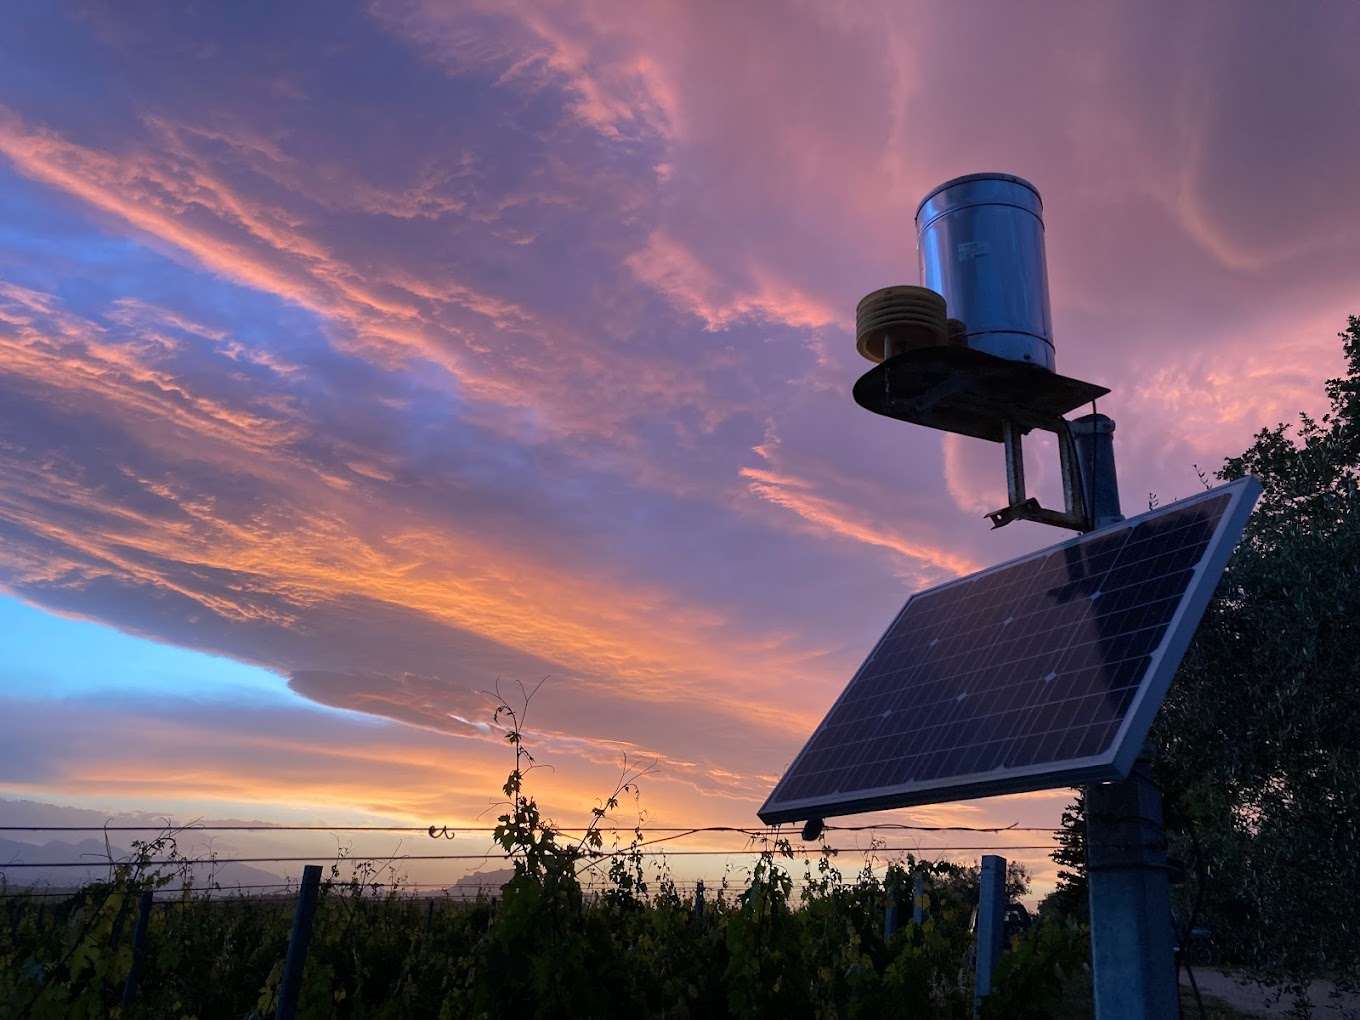
\includegraphics [width=.55\columnwidth, angle=0]
            {stazioneiot}
	\caption{La stazione IoT presente nel campo dell'azienda vitivinicola Strappelli}
	\label{3fig:foto_stazione}
\end{figure}

L'azienda Trace Technologies ha posizionato la stazione IoT nelle vicinanze della vite monitorando i seguenti valori atmosferici e valori utili con lo scopo di stabilire lo stato di salute del vigneto:

\begin{itemize}
    \item temperatura ed umidità atmosferica;
    \item millimetri di pioggia (giornalieri, del giorno precedente, istantanei e totali) misurati tramite un pluviometro posizionato nella parte superiore della stazione (è visibile un contenitore cilindrico nella figura \ref{3fig:foto_stazione});
    \item temperatura ed umidità della foglia (misurate tramite un sensore mostrato in figura \ref{3fig:leafSensor});
    \item temperatura ed umidità del terreno (misurate tramite un sensore inserito all'interno del terreno). 
\end{itemize}

\begin{figure}[h]
	\centering
	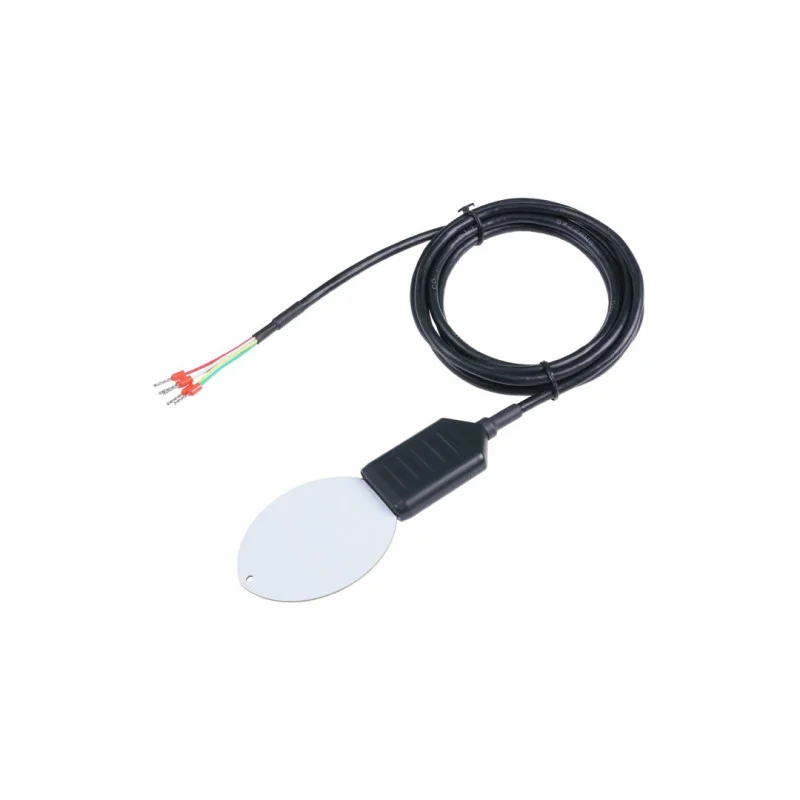
\includegraphics [width=.55\columnwidth, angle=0]
            {leafSensor}
	\caption{Sensore di temperatura ed umidità della foglia}
	\label{3fig:leafSensor}
\end{figure}

Per rendere il progetto sostenibile dal punto di vista ambientale, la stazione IoT è alimentata da un pannello fotovoltaico che durante il giorno fornisce l'energia necessaria alla stazione mentre l'energia che non viene impiegata durante le ore diurne è immagazzinata all'interno di una batteria che alimenta il sistema durante le ore notturne.

La stazione possiede inoltre un modulo 3G per la connessione ad internet tramite una scheda SIM posta al suo interno.

I dati raccolti dalla stazione vengono memorizzati localmente all'interno di una scheda SD per poi essere caricati su una piattaforma cloud che permette l'accesso dei dati da remoto tramite un'apposita API.

\section{Funzionamento dell'applicazione}

Al momento dell'avvio dell'applicazione, viene visualizzato un menu che contiene tre pulsanti. Questi ultimi consentono all'utente di selezionare quale delle tre sezioni disponibili (Osserva, Ascolta, Racconta) desidera esplorare dopo che il riconoscimento della bottiglia è stato completato. In figura \ref{3fig:menuPrincipale} è presente uno screenshot del menu appena descritto.

\begin{figure}[h]
	\centering
	
\includegraphics [width=.55\columnwidth, angle=0]
            {menuPrincipale}
	\caption{Menu principale dell'applicazione}
	\label{3fig:menuPrincipale}
\end{figure}

Dopo aver scelto la sezione di interesse, viene mostrata all'utente una schermata composta da un pulsante che permette di accedere alla scena successiva incentrata nell'attivazione della camera AR per il riconoscimento automatico del prodotto vitivinicolo. In figura \ref{3fig:toccaPerContinuare}, è mostrato il bottone che attende il tocco dell'utente prima di iniziare il riconoscimento del prodotto.

\begin{figure}[h]
	\centering
	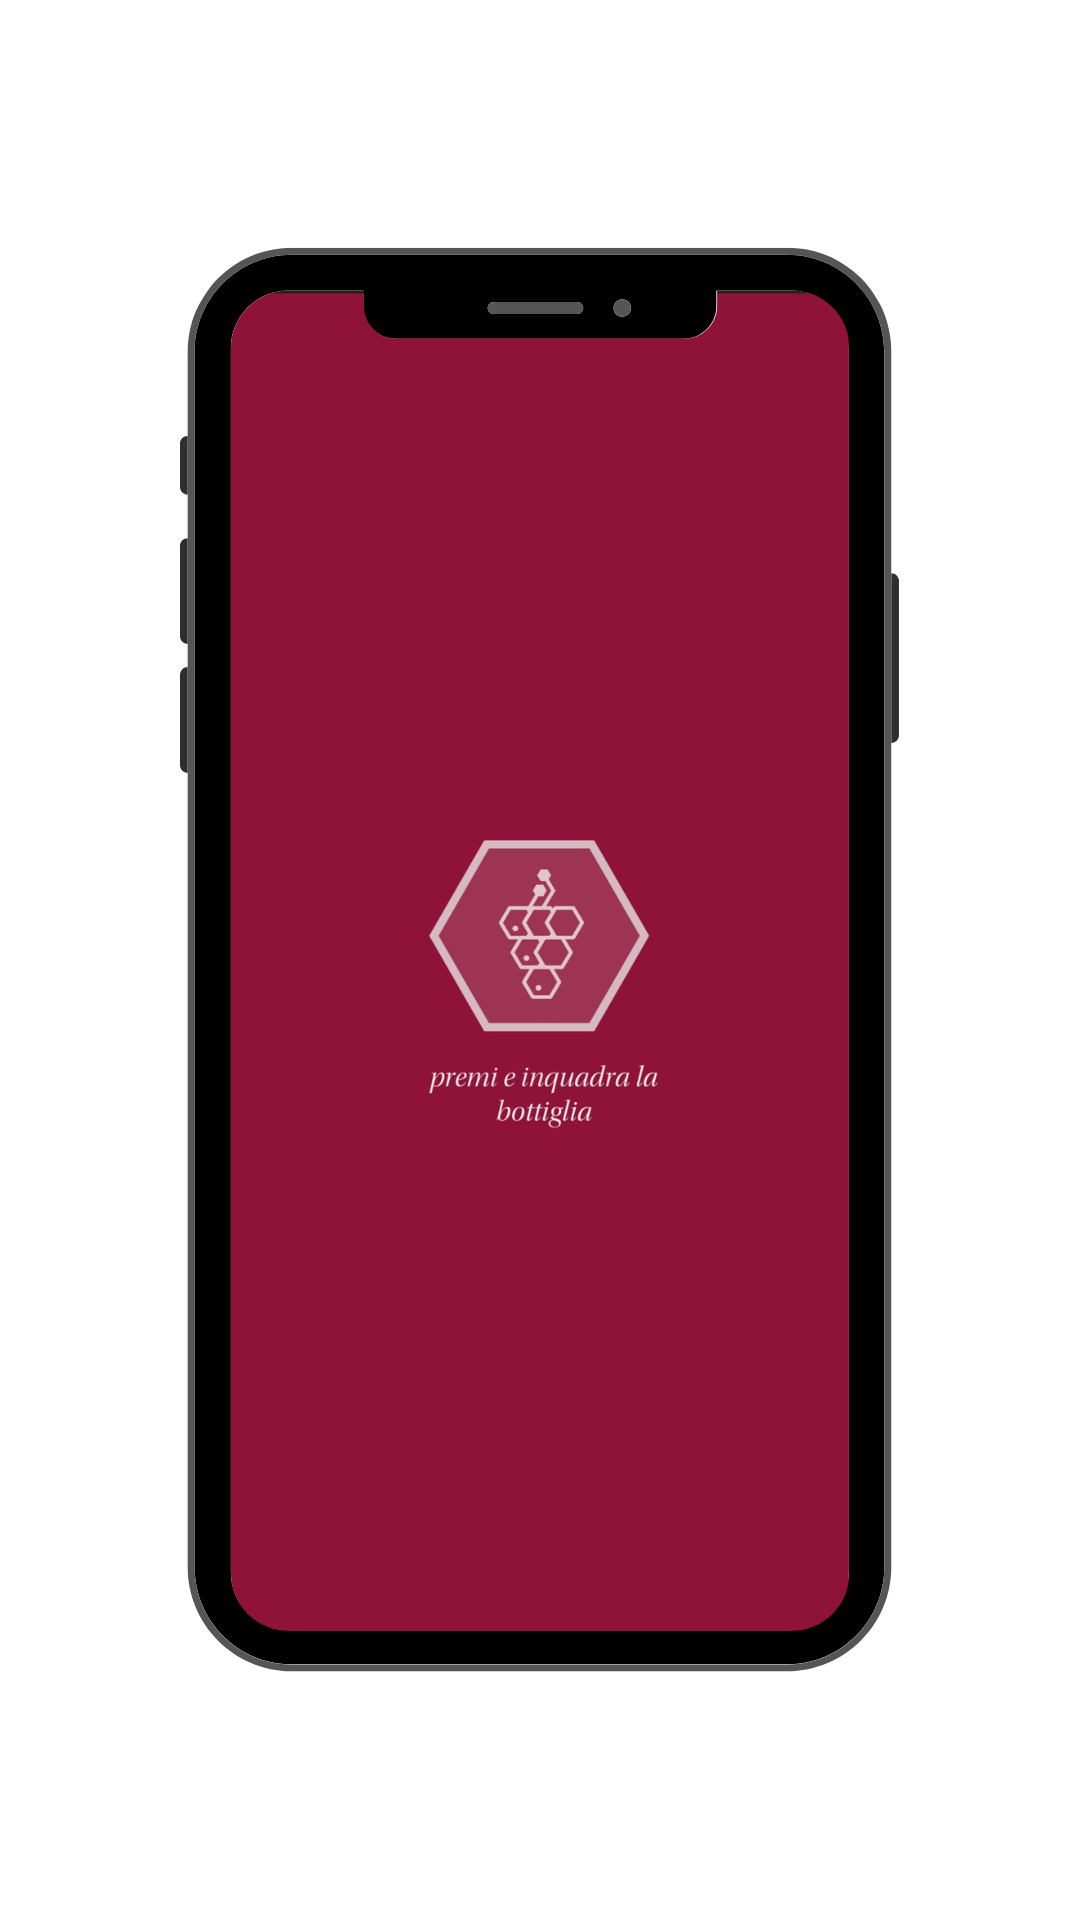
\includegraphics [width=.55\columnwidth, angle=0]
            {toccaPerContinuare}
	\caption{Pulsante che chiede all'utente di iniziare il riconoscimento del prodotto vitivinicolo}
	\label{3fig:toccaPerContinuare}
\end{figure}

Dopo aver premuto uno dei pulsanti, l'applicazione attiva la fotocamera in modalità AR e avvia la ricerca della bottiglia di vino nell'ambiente inquadrato. L'obiettivo è individuare la bottiglia e identificare l'azienda produttrice del vino. Successivamente, l'applicazione mostra le informazioni disponibili sull'azienda, fornite da Trace Technologies. In figura \ref{3fig:ScenaRiconoscimento} è mostrato uno screenshot della scena Unity.

\begin{figure}[h]
	\centering
	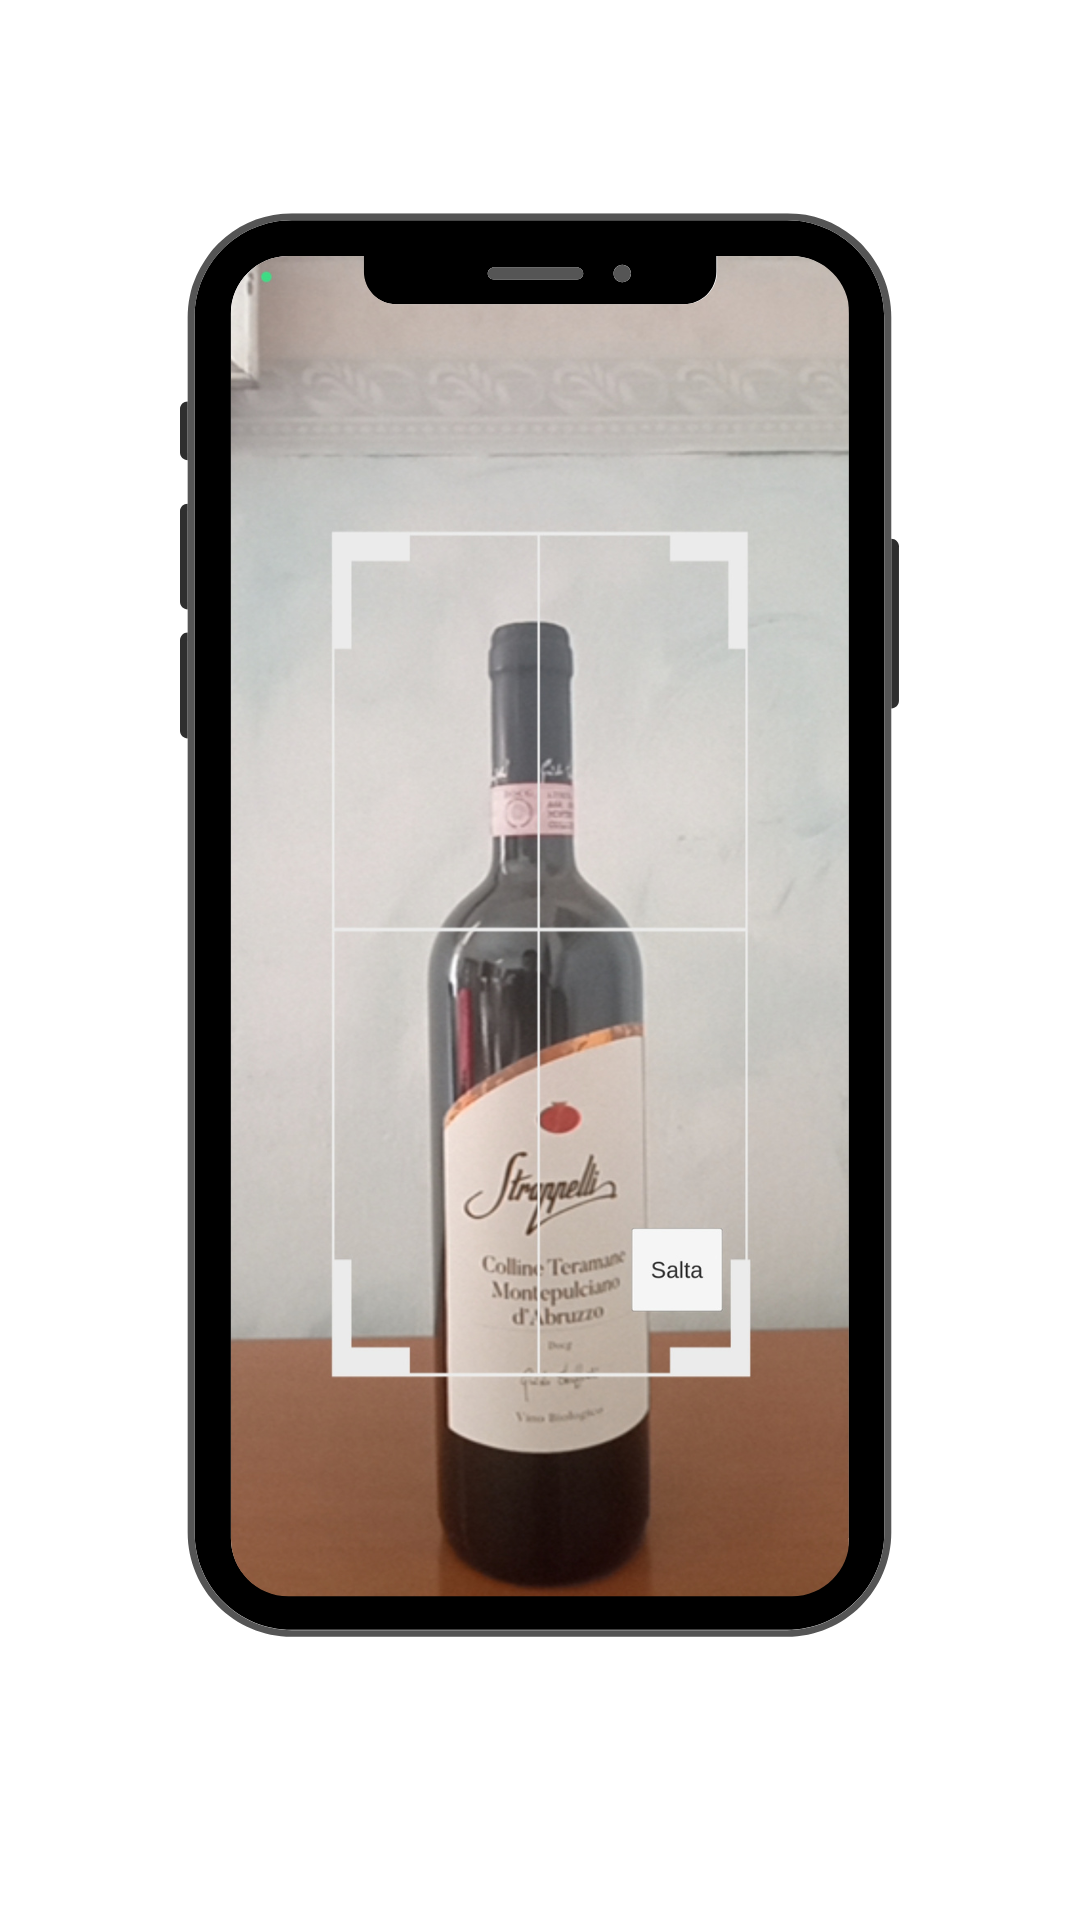
\includegraphics [width=.55\columnwidth, angle=0]
            {ScenaRiconoscimento}
	\caption{Scena AR dedicata al riconoscimento del prodotto vitivinicolo}
	\label{3fig:ScenaRiconoscimento}
\end{figure}

Per scopi dimostrativi, è stato incluso un pulsante denominato "salta" nell'applicazione, il quale consente di procedere alla scena successiva anche se la bottiglia di vino non è stata riconosciuta. In situazioni in cui l'utente non possiede effettivamente la bottiglia di vino, verrà impostata una variabile che registra il tag della bottiglia riconosciuta con il valore "Strappelli".

Una volta completato il processo di riconoscimento della bottiglia, l'applicazione Unity passa ad una nuova scena. In quest'ultima, la fotocamera rimane attiva ma l'algoritmo di riconoscimento degli oggetti viene disattivato per risparmiare risorse. Successivamente, viene mostrata una finestra a comparsa dall'alto che chiede all'utente di selezionare l'annata della bottiglia che possiede. Questa scelta implementativa è stata necessaria poiché Vuforia Engine non è sempre in grado di determinare con precisione l'annata della bottiglia dall'etichetta, poiché quest'ultima potrebbe non essere sempre chiaramente visibile.

In figura \ref{3fig:FinestraScorrevole} è mostrata la finestra scorrevole appena descritta.

\begin{figure}[h]
	\centering
	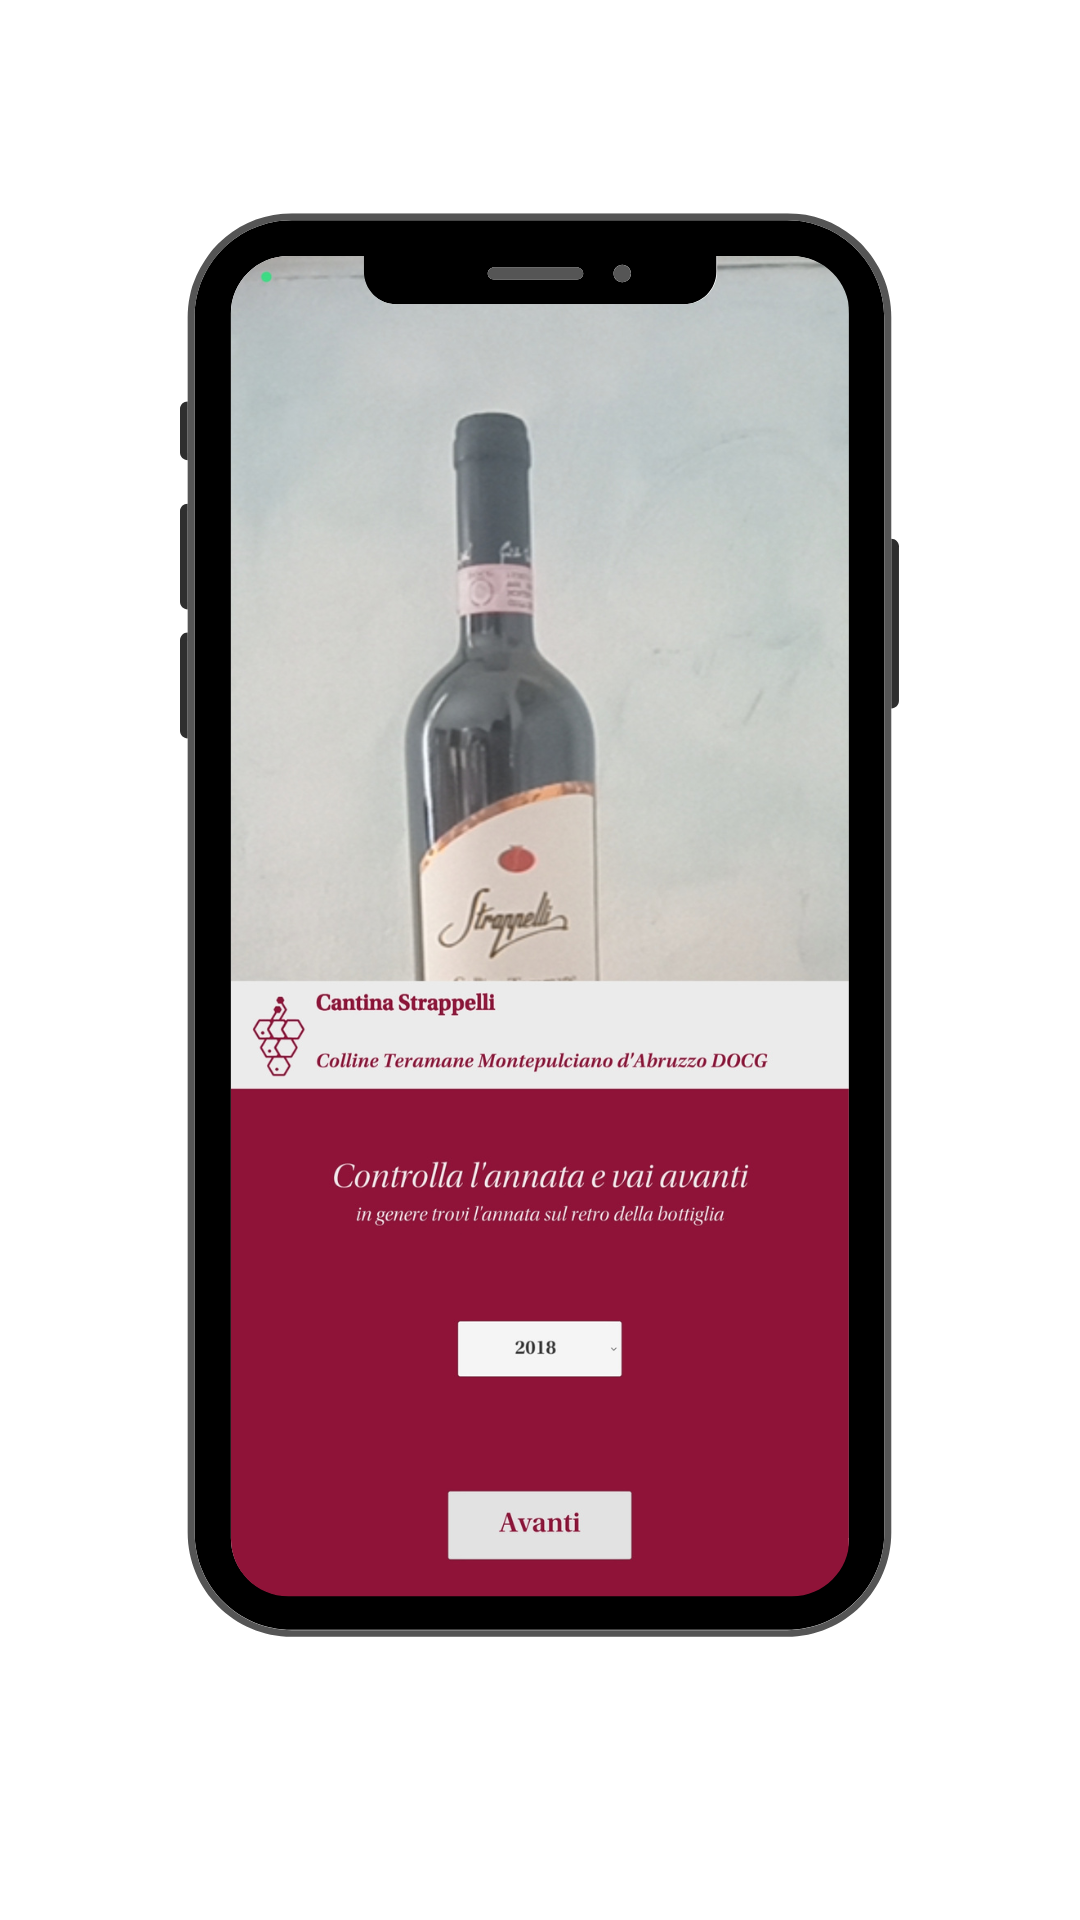
\includegraphics [width=.55\columnwidth, angle=0]
            {FinestraScorrevole}
	\caption{Finestra per la selezione dell'annata del prodotto vitivinicolo}
	\label{3fig:FinestraScorrevole}
\end{figure}

Selezionata l'annata, l'applicazione Unity carica l'ultima scena che contiene tutte le sezioni menzionate in precedenza (Osserva, Ascolta e Racconta) mostrate rispettivamente nelle figure \ref{3fig:ScenaOsserva}, \ref{3fig:ScenaAscolta} e \ref{3fig:ScenaRacconta}.

\begin{figure}[h]
	\centering
	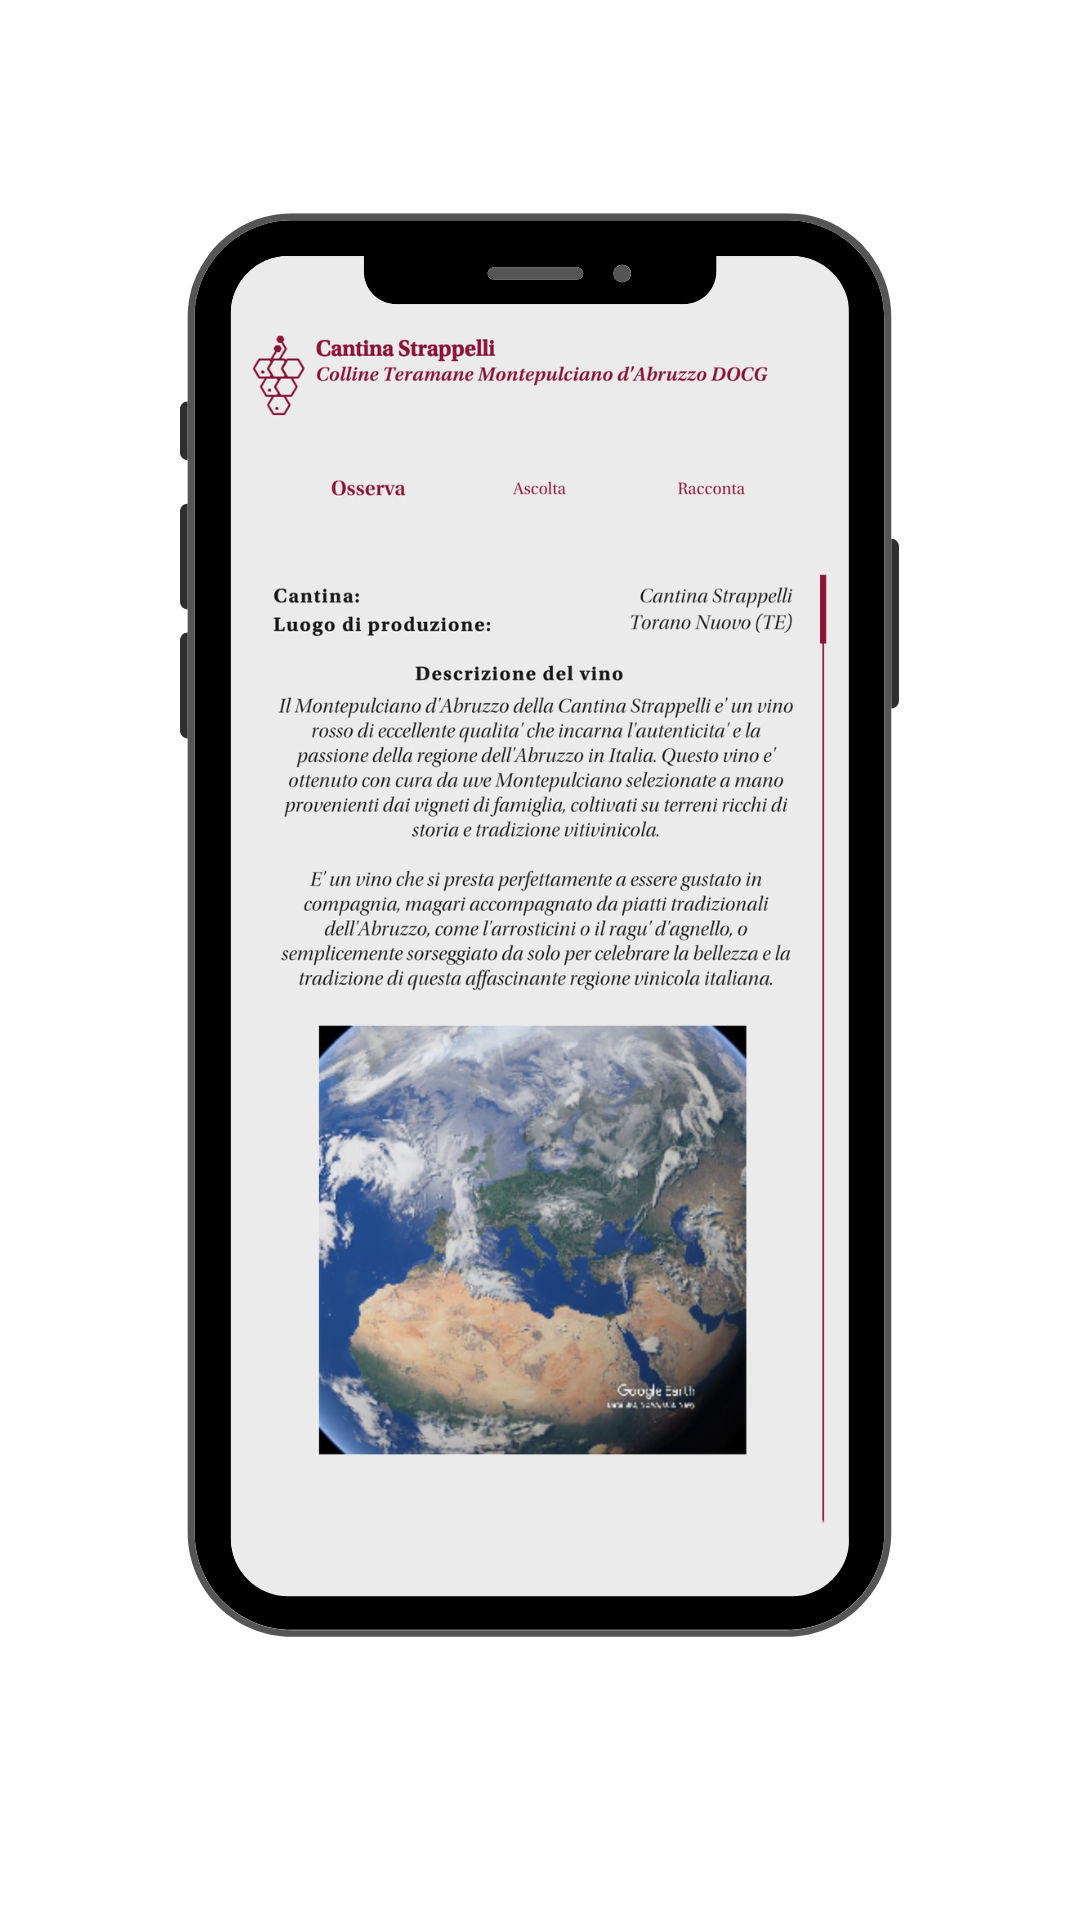
\includegraphics [width=.55\columnwidth, angle=0]
            {ScenaOsserva}
	\caption{Screenshot della sezione Osserva}
	\label{3fig:ScenaOsserva}
\end{figure}

\begin{figure}[h]
	\centering
	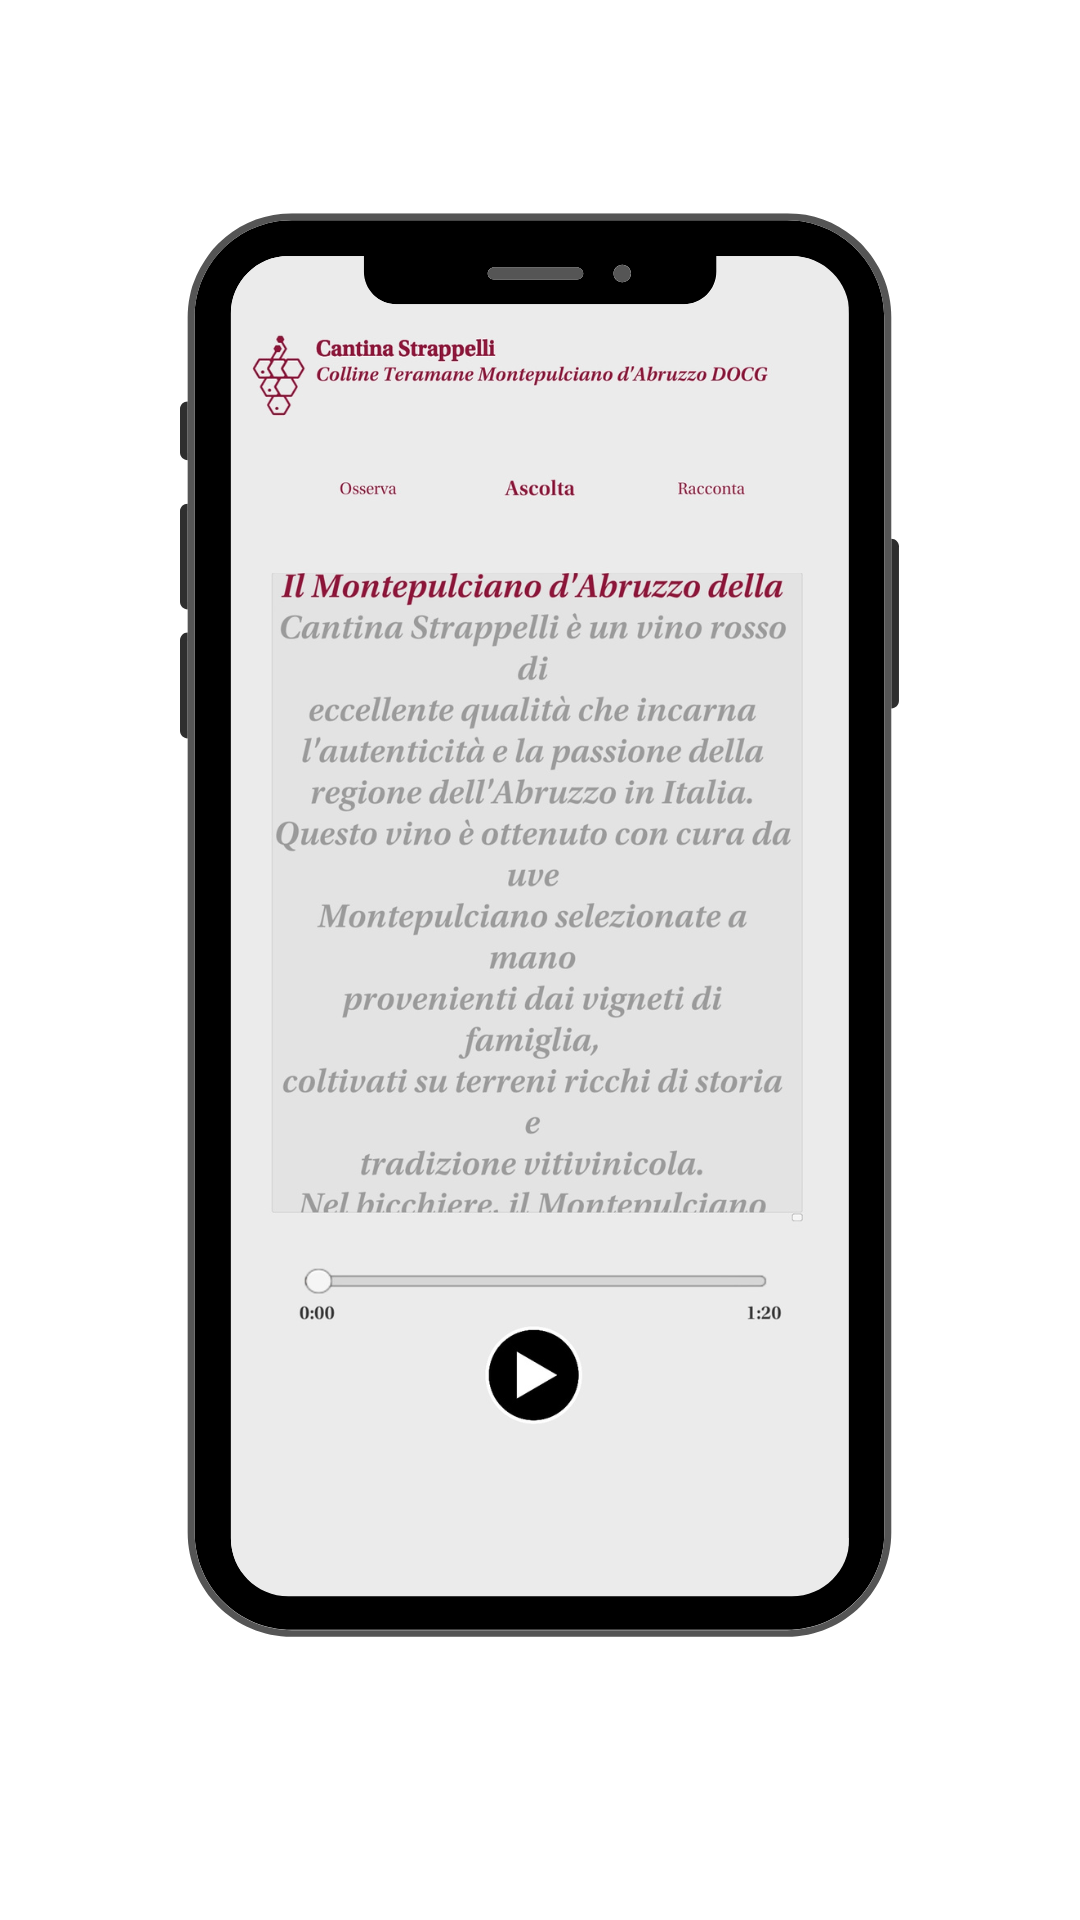
\includegraphics [width=.55\columnwidth, angle=0]
            {ScenaAscolta}
	\caption{Screenshot della sezione Ascolta}
	\label{3fig:ScenaAscolta}
\end{figure}

\begin{figure}[h]
	\centering
	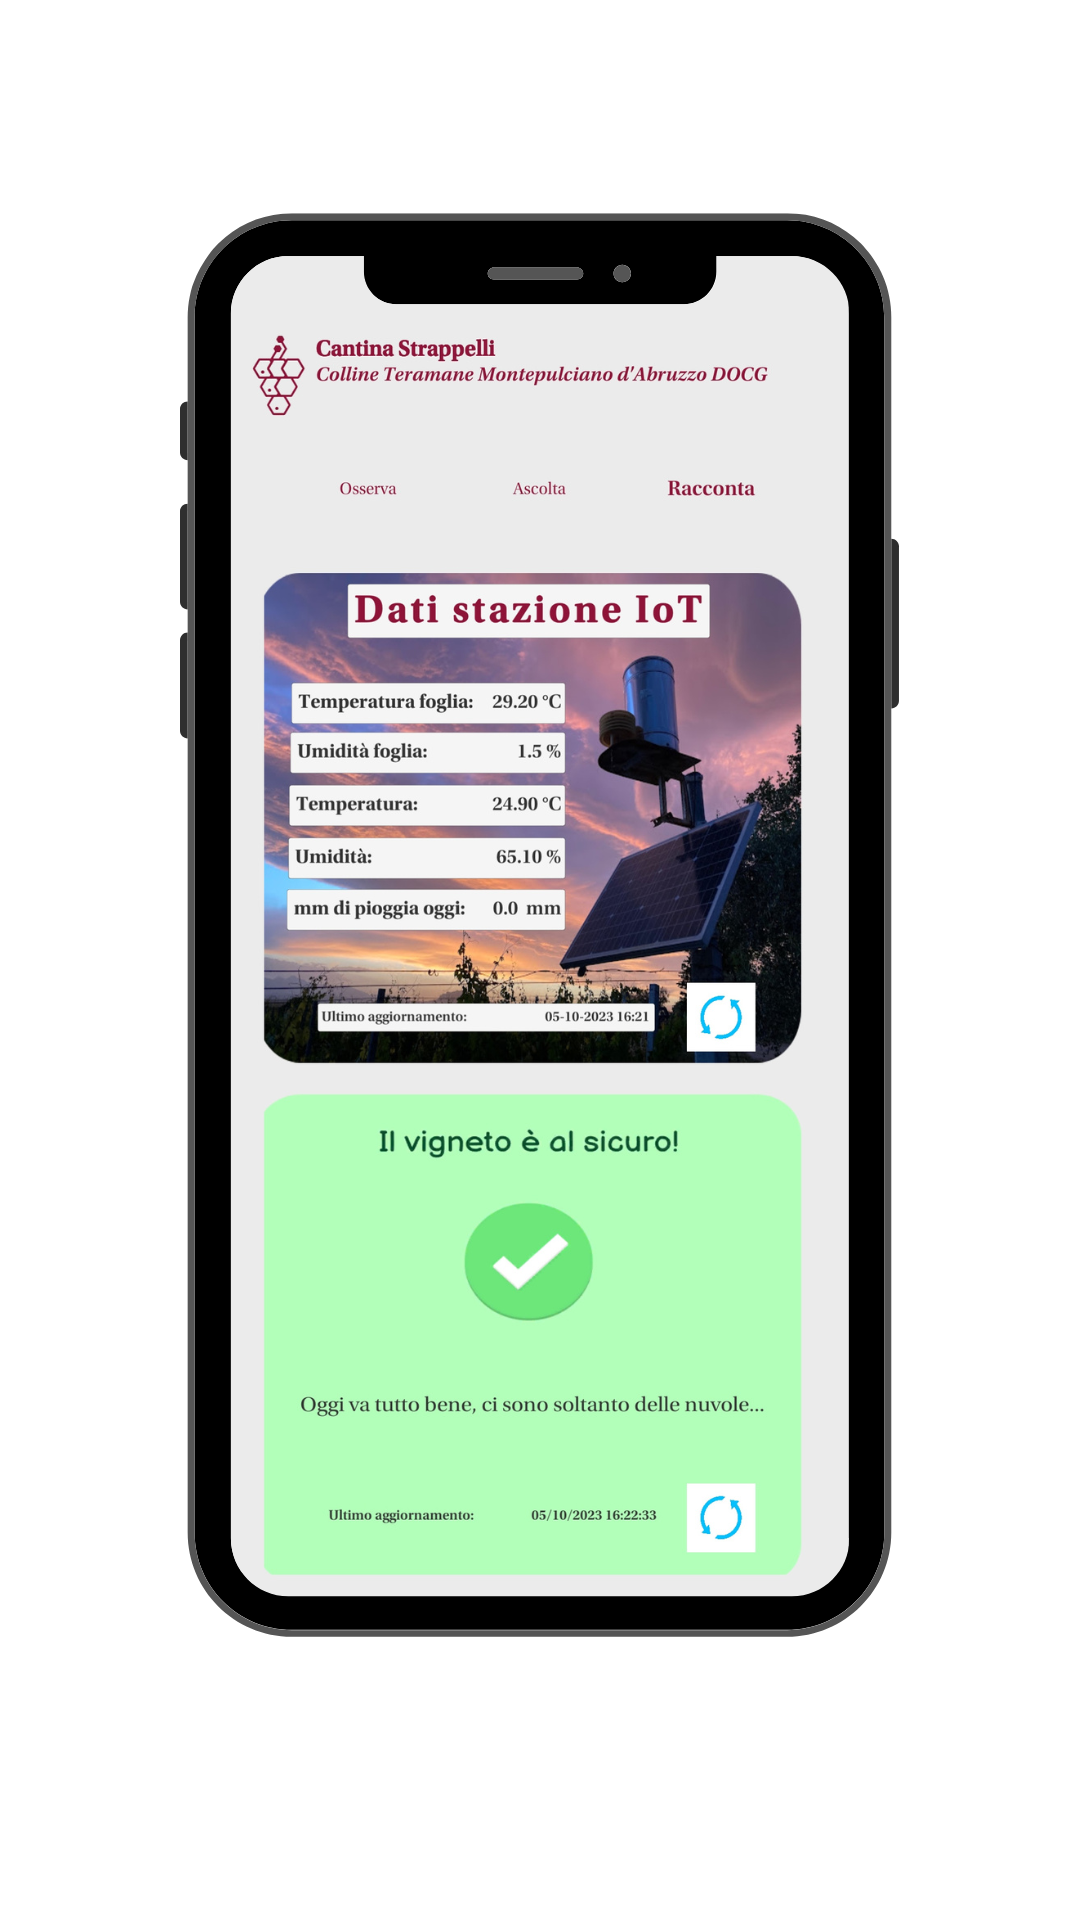
\includegraphics [width=.55\columnwidth, angle=0]
            {ScenaRacconta}
	\caption{Screenshot della sezione Racconta}
	\label{3fig:ScenaRacconta}
\end{figure}
\chapter{Progettazione del sistema}

\begin{preamble}
{\em 
In questo capitolo, si esplorerà in dettaglio la progettazione software dell'applicazione Android. Si esamineranno i diagrammi delle classi delle principali classi implementate nel progetto per fornire una visione completa della loro struttura.

Successivamente, si presenterà un diagramma di sequenza che illustrerà le interazioni dinamiche tra le classi principali implementate nell'app. Questo permetterà di comprendere in dettaglio le operazioni svolte dall'applicazione durante il processo di riconoscimento degli oggetti.

Inoltre, si descriveranno le animazioni implementate in Unity, che contribuiscono a rendere l'esperienza utente più coinvolgente e interattiva.

Per completare il quadro della progettazione, si esplorerà anche la struttura del database utilizzato per memorizzare informazioni cruciali sulle bottiglie di vino. Questa parte è essenziale per garantire un recupero e una gestione efficiente dei dati all'interno dell'app Android.
}
\end{preamble}

\section{Scelte progettuali effettuate}

Nel capitolo precedente, si è fornita una panoramica degli strumenti software utilizzati, insieme alle loro funzionalità principali. In questa sezione, si descriveranno le versioni e le modalità di utilizzo di questi strumenti, offrendo una prima documentazione progettuale dell'applicazione:

\begin{itemize}
\item \textit{Unity}: si è optato per l'utilizzo della versione dell'editor \textit{2022.3.9f1 LTS (Long-Term-Support)} al fine di garantire maggiore stabilità, rinunciando alle ultime versioni.
\item \textit{Vuforia Engine}: la versione utilizzata è la \textit{10.17.4}.
\item \textit{PolyCam}: l'applicazione offre diverse modalità d'uso, ma in questo contesto si è selezionata la \textit{Photo Mode}. Si sono acquisite oltre 100 fotografie della bottiglia della Cantina Strappelli tramite smartphone per creare un modello tridimensionale dell'oggetto, comprensivo di texture per il riconoscimento del colore e grafica dell'etichetta della bottiglia di vino.
\item \textit{Blender}: poiché non sono richieste funzionalità avanzate di Blender per il progetto, si è installata l'ultima versione disponibile, ovvero la 3.6.
\item \textit{Vuforia Model Target Generator}: anche in questo caso, si è utilizzata l'ultima versione disponibile dell'applicazione, la \textit{10.17.4}.
\item \textit{OpenWeather}: nel progetto, si è utilizzata la versione 2.5 dell'API di OpenWeather.
\end{itemize}

\section{Diagrammi delle classi}

Un \textit{diagramma delle classi} (o \textit{Class Diagram} in inglese), è uno dei diagrammi più comuni utilizzati nella modellazione dei sistemi orientati agli oggetti nell'ambito dell'ingegneria del software. Questo diagramma fa parte del linguaggio di modellazione \textit{Unified Modeling Language (UML)}, che è ampiamente utilizzato per rappresentare visivamente le strutture e le relazioni dei componenti di un sistema software.

Un diagramma delle classi contiene il nome della classe e tre sezioni principali:

\begin{itemize}
    \item \textit{Nome della classe}: è il nome della classe che rappresenta un concetto o un oggetto all'interno del sistema software;
    \item \textit{Attributi}: gli attributi sono le variabili o i campi dati che appartengono alla classe. Sono elencati sotto il nome della classe e possono includere tipi di dati e valori iniziali;
    \item \textit{Metodi}: i metodi sono le funzioni o i comportamenti associati alla classe. Sono elencati sotto gli attributi e mostrano i dettagli sulla firma dei metodi, inclusi i parametri e i tipi di ritorno.
\end{itemize}

\subsection{La classe IotAPICaller}

La classe \textit{IotAPICaller} è responsabile della gestione delle chiamate API alla stazione IoT situata nel campo dell'azienda vitivinicola Strappelli. Come precedentemente menzionato nel capitolo precedente, la stazione IoT carica i dati in tempo reale su una piattaforma cloud, la quale ospita un'appostia API che consente l'accesso ai dati.

L'API restituisce i dati in formato JSON, strutturati in modo simile ad una tabella di un database relazionale. Questa struttura comprende un'intestazione e un corpo di tabella, con l'aggiunta di due campi aggiuntivi, denominati \textit{status} e \textit{rows}.

La classe \textit{IotAPICaller} effettua una richiesta HTTP POST con una query SQL nel corpo della richiesta per ottenere i dati più recenti caricati dalla stazione IoT sulla piattaforma cloud.

Un esempio della struttura dei dati è riportato di seguito:

\begin{lstlisting}
 {
    "status":"succ",
    "head":
        [
            "ts",
            "coll_time",
            "temperature",
            "humidity",
            "rainfall_today",
            "rainfall_instantaneous",
            "rainfall_yesterday",
            "rainfall_total",
            "soil_temperature",
            "soil_moisture",
            "leaf_humidity",
            "leaf_temperature",
            "ext_str",
            "ext_var1",
            "ext_var2"
        ],
    "data":
        [
            [
                "2023-09-16 15:22:04.627",
                "2023-09-16 15:22:04.625",
                23.00000,
                89.90000,
                0.00000,
                0.00000,
                3.50000,
                3.50000,
                -3.50000,
                -2.50000,
                2.00000,
                25.30000,
                0.00000,
                0.00000,
                0.00000
            ]
        ],
    "rows":1
}
\end{lstlisting}

Il primo campo denominato \textit{"status"} mostra lo stato della richiesta HTTP inviata.
Il campo \textit{"head"}, come già accennato, rappresenta l'intestazione della tabella che descrive i dati ed è composta dai seguenti campi inseriti all'interno di un array:

\begin{itemize}
    \item \textit{ts}: rappresenta un timestamp che indica quando i dati sono stati registrati.
    \item \textit{coll\_time}: il campo rappresenta il momento in cui i dati sono stati effettivamente raccolti.
    \item \textit{temperature}: rappresenta la temperatura in gradi Celsius.
    \item \textit{humidity}: rappresenta l'umidità relativa dell'aria in percentuale. 
    \item \textit{rainfall\_today}: rappresenta la quantità di pioggia caduta durante la giornata in millimetri.
    \item \textit{rainfall\_instantaneous}: questo campo rappresenta la quantità di pioggia caduta istantaneamente al momento della raccolta dati in millimetri.
    \item \textit{rainfall\_yesterday}: rappresenta la quantità di pioggia caduta nella giornata precedente in millimetri.
    \item \textit{rainfall\_total}: questo campo rappresenta la quantità totale di pioggia caduta fino a quel momento in millimetri.
    \item \textit{soil\_temperature}: questo campo rappresenta la temperatura del suolo in gradi Celsius.
    \item \textit{soil\_moisture}: rappresenta l'umidità del suolo, probabilmente in percentuale o un'altra unità specifica.
    \item \textit{leaf\_humidity}: questo campo rappresenta l'umidità delle foglie delle piante, probabilmente in percentuale o un'altra unità specifica.
    \item \textit{leaf\_temperature}: rappresenta la temperatura delle foglie delle piante in gradi Celsius.
    \item \textit{ext\_str}, \textit{ext\_var1} e \textit{ext\_var2}: questi campi contengono dati aggiuntivi in formato numerico.
\end{itemize}

Il campo \textit{data} contiene al suo interno i valori associati all'intestazione presente nel campo \textit{head}. Infine, il campo \textit{rows} contiene il numero di righe estratte dalla query SQL.

\begin{figure}[h]
	\centering
	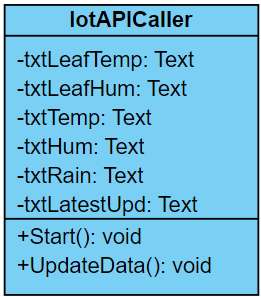
\includegraphics [width=.30\columnwidth, angle=0]
            {ClassDiagramIotAPICaller}
	\caption{Class Diagram della classe IotAPICaller}
	\label{4fig:classDiagramIotAPICaller}
\end{figure}

La classe IotAPICaller, mostrata nel Class Diagram in figura \ref{4fig:classDiagramIotAPICaller}, ha i seguenti attributi:

\begin{itemize}
    \item \textit{txtLeafTemp}: rappresenta il testo all'interno dell'interfaccia grafica di Unity relativo alla temperatura della foglia; 
    \item \textit{txtLeafHum}: rappresenta il testo all'interno dell'interfaccia grafica di Unity relativo all'umidità della foglia;
    \item \textit{txtTemp}:rappresenta il testo all'interno dell'interfaccia grafica di Unity relativo alla temperatura atmosferica;
    \item \textit{txtHum}: rappresenta il testo all'interno dell'interfaccia grafica di Unity relativo all'umidità atmosferica;
    \item \textit{txtRain}: rappresenta il testo all'interno dell'interfaccia grafica di Unity relativo ai millimetri di pioggia giornalieri;
    \item \textit{txtLatestUpd}: rappresenta il testo all'interno dell'interfaccia grafica di Unity relativo al timestamo dei dati presentati nell'applicazione.
\end{itemize}

Ogni variabile ha l'attributo \textit{SerializeField} per renderla privata e visibile nell'editor di Unity in modo che possa essere vista e modificata nel valore direttamente nell'interfaccia grafica, anche se il campo è dichiarato come privato.

Infine, la classe contiene i seguenti metodi:

\begin{itemize}
    \item \textit{Start}: è il primo metodo che viene eseguito all'avvio dello script nella pagina "Racconta" dell'applicazione. La chiamata a questo metodo permette di preparare la richiesta HTTP in modo corretto inserendo l'intestazione della chiamata HTTP e il body con il testo della query SQL che permette di recuperare i dati;
    \item \textit{UpdateData}: questo metodo permette di eseguire un'ulteriore chiamata API per consentire un aggiornamento dei dati visualizzati nell'applicazione.
\end{itemize}

\subsection{La classe OpenWeatherAPICaller}

La classe \textit{OpenWeatherAPICaller} si occupa di gestire i dati che provengono dall'API di OpenWeather. Quest'ultima restituisce i dati in formato JSON. Un esempio è fornito di seguito:

\begin{lstlisting}
{
    "coord":
            {
                "lon": 13.7589,
                "lat": 42.8142
            },
    "weather":
            [
                {
                    "id": 800,
                    "main": "Clear",
                    "description": "clear sky",
                    "icon": "01d"
                }
            ],
    "base": "stations",
    "main":
            {
                "temp": 299.41,
                "feels_like": 299.41,
                "temp_min": 295.96,
                "temp_max": 301.19,
                "pressure": 1016,
                "humidity": 65,
                "sea_level": 1016,
                "grnd_level": 992
            },
    "visibility": 10000,
    "wind":
            {
                "speed": 3.41,
                "deg": 62,
                "gust": 2.6
            },
    "clouds":
            {
                "all": 0
            },
    "dt": 1694272098,
    "sys":
            {
                "type": 2,
                "id": 2006527,
                "country": "IT",
                "sunrise": 1694234268,
                "sunset": 1694280450
            },
    "timezone": 7200,
    "id": 3165549,
    "name": "Torano Nuovo",
    "cod": 200
} 
\end{lstlisting}

Il file JSON presenta diversi campi tra cui:

\begin{itemize}
    \item \textit{coord}: questo campo contiene le coordinate geografiche della località.
    \begin{itemize}
        \item \textit{lon}: il campo rappresenta la longitudine del campo da monitorare.
        \item \textit{lat}: il campo rappresenta la latitudine del campo da monitorare.
    \end{itemize}

    \item \textit{weather}: questo campo contiene informazioni sulle condizioni meteorologiche attuali.
    \begin{itemize}
        \item \textit{id}: è un codice numerico che rappresenta il tipo di condizione meteorologica.
        \item \textit{main}: racchiude una descrizione categorica del meteo in attuale.
        \item \textit{description}: descrizione più dettagliata della condizione meteo.
        \item \textit{icon}: rappresenta un'icona associata alle condizioni meteorologiche.
    \end{itemize}
    \item \textit{base}: specifica la stazione meteorologica di riferimento.
    \item \textit{main}: questo campo contiene informazioni sulle condizioni meteorologiche principali.
    \begin{itemize}
        \item \textit{temp}: rappresenta la temperatura attuale in gradi Celsius.
        \item \textit{feels\_like}: rappresenta la temperatura percepita in gradi Celsius.
        \item \textit{temp\_min}: rappresenta la temperatura minima prevista in gradi Celsius.
        \item \textit{temp\_max}: immagazzina la temperatura massima prevista in gradi Celsius.
        \item \textit{pressure}: questo campo rappresenta la pressione atmosferica in hPa.
        \item \textit{humidity}: rappresenta l'umidità relativa in percentuale.
        \item \textit{sea\_level}: questo campo rappresenta la pressione al livello del mare in hPa.
        \item \textit{grnd\_level}: rappresenta la pressione al livello del suolo in hPa.
    \end{itemize}
        
    \item \textit{visibility}: rappresenta la visibilità attuale in metri.
    \item \textit{wind}: questo campo contiene informazioni sul vento.
    \begin{itemize}
        \item \textit{speed}: rappresenta la velocità del vento in metri al secondo.
        \item \textit{deg}: rappresenta la direzione del vento in gradi.
        \item \textit{gust}: questo campo rappresenta la velocità delle raffiche di vento in metri al secondo.
    \end{itemize}
    
    \item \textit{clouds}: questo campo fornisce informazioni sulle nuvole.
    \begin{itemize}
        \item \textit{all}: rappresenta la copertura nuvolosa in percentuale.
    \end{itemize}
        
    \item \textit{dt}: è il timestamp Unix che rappresenta il momento in cui sono stati acquisiti questi dati meteorologici.
    \item \textit{sys}: questo campo contiene informazioni sul sistema.
    \begin{itemize}
        \item \textit{type}: è tipo di sistema.
        \item \textit{id}: rappresenta l'ID del sistema.
        \item \textit{country}: rappresenta il paese associato a questa località.
        \item \textit{sunrise}: rappresneta il timestamp Unix del sorgere del sole.
        \item \textit{sunset}: questo campo rappresenta il timestamp Unix del tramonto.
    \end{itemize}
        
    \item \textit{timezone}: è il fuso orario della località in secondi rispetto all'UTC. 
    \item \textit{id}: rappresenta l'ID univoco associato alla località.
    \item \textit{name}: è il nome della località.
    \item \textit{cod}: rappresenta lo stato della richiesta HTTP.
\end{itemize}

\begin{figure}[h]
	\centering
	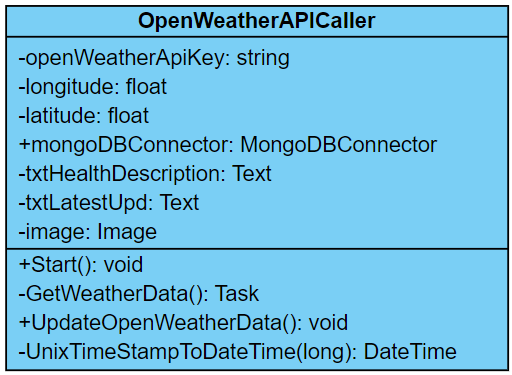
\includegraphics [width=.55\columnwidth, angle=0]
            {ClassDiagramOpenWeatherAPICaller}
	\caption{Class Diagram della classe OpenWeatherAPICaller}
	\label{4fig:classDiagramOpenWeatherAPICaller}
\end{figure}

La classe \textit{OpenWeatherAPICaller} ha il compito di trasformare la stringa JSON proveniente dall'API di OpenWeather in una serie di variabili, ciascuna corrispondente a un campo del file JSON.

Per svolgere questa operazione, fa uso di classi strutturate in modo da organizzare e incapsulare i dati relativi alle condizioni meteorologiche in una forma facilmente gestibile all'interno dell'applicazione. La classe principale, denominata \textit{WeatherData}, raccoglie tutti i dati relativi alle condizioni meteorologiche, mentre le altre classi vengono impiegate per rappresentare informazioni specifiche all'interno di questa struttura dati gerarchica.

Le proprietà presenti nella classe OpenWeatherAPICaller sono:

\begin{itemize}
    \item \textit{openWeatherApiKey}: contiene la chiave che consente l'utilizzo dell'API OpenWeather;
    \item \textit{longitude}: questa proprietà contiene la longitudine del campo da monitorare;
    \item \textit{latitude}: questa proprietà contiene la latitudine del campo da monitorare;
    \item \textit{mongoDBConnector}: contiene l'istanza della classe MongoDBConnector che si occupa di gestire la connessione con il database MongoDB (verrà descritta approfonditamente in seguito);
    \item \textit{txtHealthDescription}: rappresenta il testo all'interno dell'interfaccia grafica di Unity relativo alla descrizione sistetica dello stato di salute del vigneto;
    \item \textit{txtLatestUpd}: rappresenta il testo all'interno dell'interfaccia grafica di Unity relativo all'ultimo aggiornamento dei dati ottenuti dall'API OpenWeather;
    \item \textit{image}: contiene il riferimento all'immagine presente nell'interfaccia grafica Unity che mostra due tipologie di immagini in base allo stato del vigneto (in salute o in stato di allerta);
\end{itemize}

Per quanto riguarda i metodi presenti nella classe, sono riportati di seguito:

\begin{itemize}
    \item \textit{Start()}: è il metodo che viene eseguito per prima nel lancio dello script in Unity. Il metodo si occupa di recuperare dal database la longitudine e latitudine del campo associato alla bottiglia di vino riconosciuta;
    \item \textit{GetWeatherData()}: il metodo si occupa di effettuare la chiamata all'API di OpenWeather per poi memorizzare i risultati nelle variabili associate a ciascun campo della stringa JSON restituita dall'API;
    \item \textit{UpdateOpenWeatherData}: aggiorna i dati provenienti all'API di OpenWeather richiamando il metodo \textit{GetWeatherData};
    \item \textit{UnixTimeStampToDateTime}: è un metodo che converte un timestamo Unix in una data nel formato \textit{DateTime}.
\end{itemize}

\subsection{La classe ScriptManager}

La classe \textit{ScriptManager} si occupa di gestire la sincronizzazione del testo con l'audio della recensione del sommelier. Il Class Diagram è mostrato nella figura \ref{4fig:classDiagramScriptManager}.

\begin{figure}[h]
	\centering
	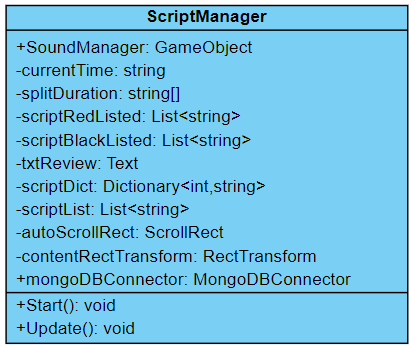
\includegraphics [width=.55\columnwidth, angle=0]
            {ClassDiagramScriptManager}
	\caption{Class Diagram della classe ScriptManager}
	\label{4fig:classDiagramScriptManager}
\end{figure}

Gli attributi della classe sono:

\begin{itemize}
    \item \textit{SoundManager}: questo attributo rappresenta l'oggetto gestisce la riproduzione audio nella scena Unity.
    \item \textit{currentTime}: è un attributo che memorizza i secondi di riproduzione attuali dell'audio in riproduzione. 
    \item \textit{splitDuration}: è un array di stringhe utilizzato per suddividere la variabile \textit{currentTime} in minuti e secondi.
    \item \textit{scriptRedListed}: questo attributo rappresenta una lista di stringhe per memorizzare frammenti di script che devono essere visualizzati in rosso. Essi rappresentano la porzione di testo già riprodotto.
    \item \textit{scriptBlackListed}: l'attributo rappresenta una lista di stringhe per memorizzare frammenti di script ancora non riprodotti.
    \item \textit{txtReview}: rappresenta un riferimento ad un componente di testo Unity utilizzato per visualizzare il testo associato allo script del sommelier.
    \item \textit{scriptDict}: rappresenta un dizionario che memorizza coppie di valori, dove la chiave è un intero (i secondi) e il valore è una stringa (il testo dello script associato a quel secondo).
    \item \textit{scriptList}: rappresenta una lista di stringhe per memorizzare l'intero script.
    \item \textit{autoScrollRect}: l'attributo rappresenta un riferimento ad un componente Unity ScrollRect. Questo attributo è serializzato in modo che possa essere assegnato nell'editor Unity. 
    \item \textit{contentRectTransform}: rappresenta un riferimento ad un componente Unity RectTransform utilizzato per gestire il layout del contenuto all'interno del ScrollRect.
    \item \textit{mongoDBConnector}: rappredenta un oggetto della classe \textit{MongoDBConnector} utilizzato per ottenere dati dal database MongoDB.
\end{itemize}

I metodi presenti nella classe sono i seguenti:

\begin{itemize}
    \item \textit{Start()}: questo metodo è chiamato all'avvio del GameObject. In particolare, acquisisce il testo della recensione associata alla bottiglia riconosciuta dal database MongoDB e visualizza il testo nello script nella variabile txtRecensione.
    \item \textit{Update()}:Questo metodo è chiamato ad ogni frame dell'applicazione. Calcola il tempo corrente, identifica i frammenti di script da evidenziare in base al tempo corrente di esecuzione dell'audio della recensione, aggiorna il testo in txtRecensione, calcola la posizione di scorrimento verticale per la visibilità del testo evidenziato e aggiorna il valore della barra di scorrimento verticale del componente autoScrollRect in base alla posizione del testo evidenziato.
\end{itemize}

\subsection{La classe MongoDBConnector}

La classe \textit{MongoDBConnector} si occupa di gestire la connessione con il database MongoDB che contiene i dati relativi al prodotto vitivinicolo identificato. La struttura del database verrà descritta in seguito.

In figura \ref{4fig:classDiagramMongoDBConnector} è mostrato il Class Diagram della classe MongoDBConnector di cui si andranno a descrivere attributi e metodi presenti.

La classe presenta quattro attributi, tra cui:

\begin{itemize}
    \item \textit{apiKey}: contiene la chiave API che consente di accedere al database MongoDB;
    \item \textit{url}: l'attributo contiene l'URL dell'API di MongoDB che consente di effettuare la ricerca nel database di un particolare record con l'operazione \textit{findOne};
    \item \textit{jsonData}: contiene un attributo che memorizza i dati JSON da inviare nel corpo della richiesta HTTP all'API di MongoDB;
    \item \textit{onDataReceived}: memorizza un attributo che contiene una funzione di callback da eseguire quando vengono ricevuti i dati dal database MongoDB.
\end{itemize}

\begin{figure}[h]
	\centering
	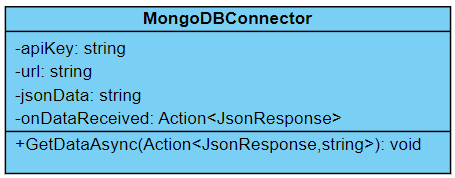
\includegraphics [width=.55\columnwidth, angle=0]
            {ClassDiagramMongoDBConnector}
	\caption{Class Diagram della classe MongoDBConnector}
	\label{4fig:classDiagramMongoDBConnector}
\end{figure}

La classe contiene un solo metodo chiamato \textit{GetDataAsync} utilizzato per avviare un processo di recupero dati asincrono che accetta due parametri:

\begin{itemize}
    \item \textit{callback}: un oggetto di tipo Action che specifica la funzione di callback da eseguire quando vengono ricevuti dati;
    \item \textit{queryType}: una stringa che specifica il tipo di query da eseguire.
\end{itemize}

All'interno di questo metodo, viene costruita una stringa di richiesta JSON in base al tipo di query richiesta, e i dati pertinenti vengono ottenuti dal database MongoDB utilizzando un oggetto \textit{UnityWebRequest}. Successivamente, la risposta viene elaborata. Se la richiesta ha successo, la risposta JSON dal database viene deserializzata in un oggetto \textit{JsonResponse} e quindi passata alla funzione di callback specificata in \textit{onDataReceived}. Nel caso in cui la richiesta non abbia successo, viene registrato un messaggio di errore e la funzione di callback viene chiamata con un parametro nullo per indicare la presenza di un errore.

\section{Sequence Diagram}

\subsection{Introduzione}

Un \textit{diagramma di sequenza} o \textit{Sequence Diagram} è uno dei diagrammi \textit{UML (Unified Modeling Language)} utilizzati nella progettazione del software e nell'analisi dei sistemi. Questo tipo di diagramma viene utilizzato per visualizzare l'interazione tra oggetti o componenti all'interno di un sistema in un momento specifico nel tempo. In altre parole, mostra come gli oggetti comunicano tra loro e in che sequenza avvengono queste interazioni.

Di seguito, verranno illustrati alcuni elementi chiave che si possono trovare in un diagramma di sequenza:

\begin{itemize}
    \item \textit{Oggetti}: rappresentano le entità o le componenti del sistema coinvolte nell'interazione.
    \item \textit{Linee di vita}: sono linee verticali che si estendono dagli oggetti e rappresentano il periodo di tempo in cui un oggetto è attivo e coinvolto nell'interazione.
    \item \textit{Messaggi}: sono frecce orizzontali che collegano gli oggetti e rappresentano le comunicazioni o le chiamate di metodo tra gli oggetti. Possono essere annotate con informazioni aggiuntive, come i parametri dei metodi chiamati.
    \item \textit{Attivazioni}: sono rappresentate da barre verticali sopra una linea di vita e indicano il periodo in cui un oggetto sta eseguendo una determinata operazione o un metodo.
\end{itemize}

I diagrammi di sequenza sono utili per comprendere il comportamento dinamico di un sistema e per identificare potenziali problemi o inefficienze nelle interazioni tra gli oggetti. Sono ampiamente utilizzati nella fase di progettazione e analisi dei sistemi software per documentare e comunicare le interazioni tra le parti del sistema.

\subsection{Sequence Diagram del progetto}

Nel Sequence Diagram in figura \ref{4fig:sequenceDiagram}, viene mostrato il flusso di esecuzione standard che va dalla visualizzazione del menu principale fino alla pagina dedicata alla sezione desiderata dall'utente.

\begin{figure}[h]
	\centering
	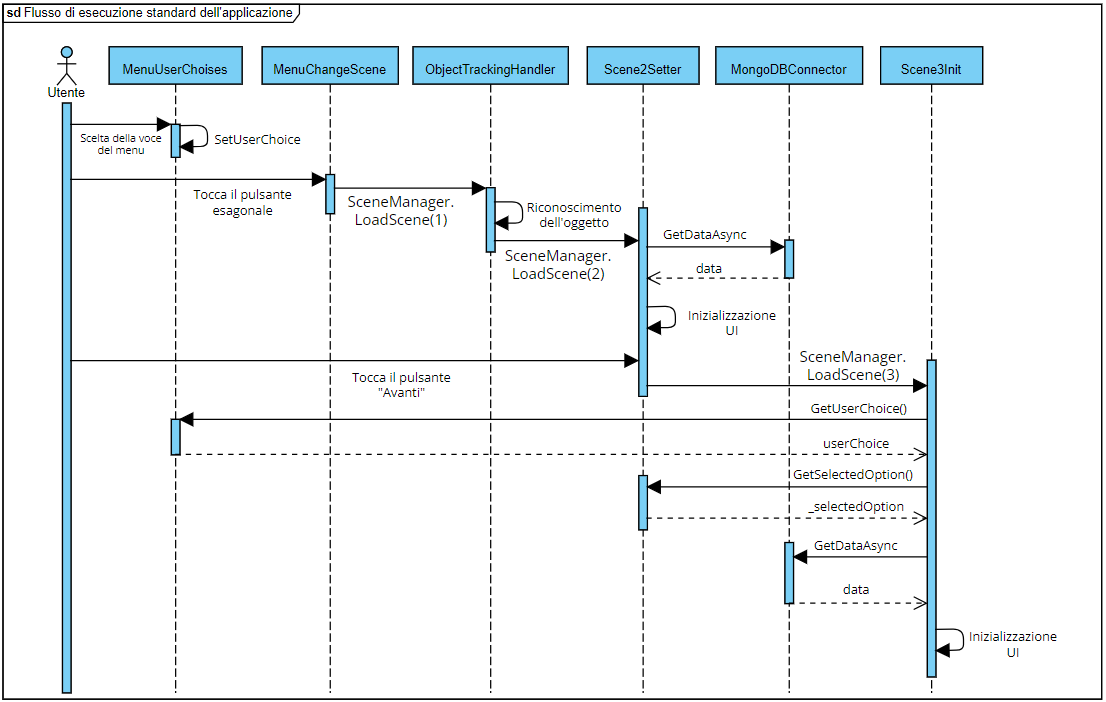
\includegraphics [width=.99\columnwidth, angle=0]
            {SequenceDiagram}
	\caption{Sequence Diagram del flusso di esecuzione principale dell'applicazione}
	\label{4fig:sequenceDiagram}
\end{figure}

Come precedentemente menzionato, il flusso dell'applicazione procede in questo modo:

Dopo che l'animazione del menu principale ha visualizzato le tre opzioni relative alle sezioni "Osserva", "Ascolta" e "Racconta", l'utente seleziona il pulsante corrispondente alla sezione di suo interesse. La classe \textit{MenuChangeChoices}, attraverso il metodo \textit{SetUserChoice}, registra il nome della sezione desiderata nella variabile \textit{userChoice}. Successivamente, l'animazione mostra il pulsante esagonale che consente di passare alla scena successiva dedicata al riconoscimento del prodotto vitivinicolo tramite il comando \textit{SceneManager.LoadScene(1)}.

L'utente accede quindi alla scena dedicata al riconoscimento del prodotto vitivinicolo. Una volta che l'oggetto è stato riconosciuto, la classe \textit{ObjectTrackingHandler} esegue il comando \textit{SceneManager.LoadScene(2)} per caricare la scena successiva.

Nella nuova scena, vengono richiesti i dati relativi alla bottiglia di vino riconosciuta al database MongoDB. Questi dati vengono utilizzati per popolare i campi testuali presenti nell'interfaccia grafica di Unity, come il nome della cantina e la qualità del vino.

Una volta che la scena è stata inizializzata correttamente con i dati relativi al prodotto vitivinicolo, l'utente seleziona l'annata desiderata e preme il pulsante "Avanti", il che avvia il caricamento dell'ultima scena dell'applicazione chiamata \textit{SceneManager.LoadScene(3)}.

All'avvio dell'ultima scena dell'applicazione, questa richiede alla classe \textit{MenuUserChoices} tramite il metodo pubblico \textit{GetUserChoice}, la stringa contenente la scelta effettuata dall'utente nel menu principale, precedentemente memorizzata nella variabile \textit{userChoice}. Successivamente, la classe \textit{Scene3Init} acquisisce l'annata scelta dall'utente tramite il metodo \textit{GetSelectedOption} e utilizza questi dati per popolare gli elementi dell'interfaccia grafica, richiedendo ulteriori informazioni alla classe \textit{MongoDBConnector}.


\section{Animazioni in Unity}

\subsection{Introduzione}

Le animazioni in Unity sono un elemento fondamentale per creare giochi interattivi e applicazioni. Le animazioni consentono di far muovere gli oggetti, i personaggi, le telecamere e molto altro all'interno del progetto Unity.

Di seguito, è riportata una panoramica del funzionamento delle animazioni in Unity:

\begin{itemize}
    \item \textit{Animator Controller}: è il componente principale per gestire le animazioni in Unity. Questo controller definisce gli stati, le transizioni e le regole per la riproduzione delle animazioni;
    \item Animation Clips: Un Animation Clip è un file che contiene un'animazione specifica. Puoi crearli importando file da programmi di modellazione 3D o crearli direttamente in Unity utilizzando l'Editor di animazione. Questi clip vengono poi collegati all'Animator Controller.
    \item \textit{Animator Window}: è un'interfaccia utente visuale che consente di creare e gestire le transizioni tra gli stati dell'Animator Controller. È possibile aggiungere transizioni tra diversi stati e definire le condizioni che le attivano.
    \item \textit{Layers}: gli Animator Controller possono avere più layer, che consentono di gestire animazioni sovrapposte o di priorità diverse.
    \item \textit{Blend Trees}: consentono di miscelare più animazioni in base a valori specifici, come direzione e velocità. Questi sono utili per controllare animazioni complesse.
    \item \textit{Parametri}: consentono di utilizzare parametri per controllare le transizioni tra gli stati.
    \item \textit{Scripting}: è possibile controllare l'animazione tramite script C\# in Unity.
    \item \textit{Importazione di animazioni}: è possibile importare animazioni create in programmi come Blender e collegarle all'Animator Controller.
    \item \textit{Esecuzione in tempo reale}: le animazioni in Unity possono essere eseguite in tempo reale, consentendo interazioni dinamiche con il mondo di gioco.
\end{itemize}

\subsection{Le animazioni utilizzate nel progetto}

\subsubsection{Menu principale}

\begin{figure}[h]
	\centering
	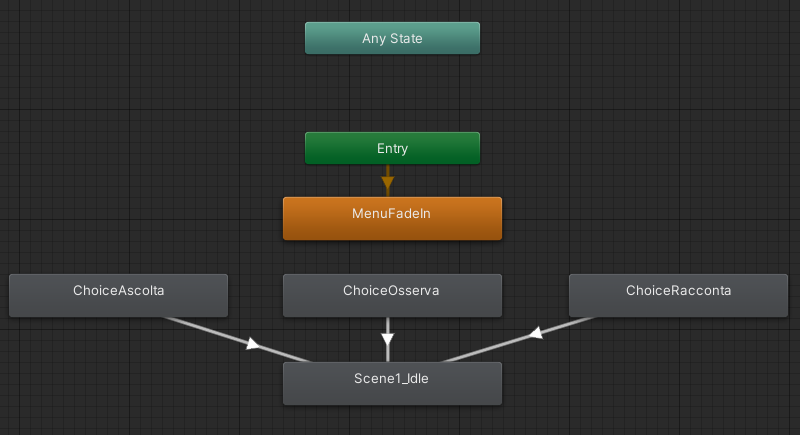
\includegraphics [width=.95\columnwidth, angle=0]
            {menuAnimSchema}
	\caption{La struttura dell'animator controller "Menu Controller"} 
	\label{4fig:menuAnimSchema}
\end{figure}

In figura \ref{4fig:menuAnimSchema}, è riportata la struttura dell'animator controller denominato \textit{Menu Controller}. Nel momento in cui l'applicazione Android viene eseguita, l'animator che si trova nello stato \textit{Entry}, attiva automaticamente l'animazione \textit{MenuFadeIn} che permette di visualizzare le tre voci del menu principale descritte nei capitoli precedenti con un effetto \textit{FadeIn} in ingresso.

Successivamente, l'applicazione rimane in attesa di un input da parte dell'utente. Quest'ultimo, nel momento in cui effettua la scelta, attiva l'animazione associata alle tre voci presenti nel menu rispettivamente \textit{ChoiceOsserva}, \textit{ChoiceAscolta} e \textit{ChoiceRacconta}. Ciascuna di queste animazioni passano automaticamente allo stato \textit{Scene1\_Idle}. 

L'applicazione mostrerà un bottone a forma di esagono che attende l'input dell'utente. Nel momento in cui il bottone verrà premuto, si attiverà la scena dedicata al riconoscimento del prodotto vitivinicolo.

\subsubsection{Scelta dell'annata}

\begin{figure}[h]
	\centering
	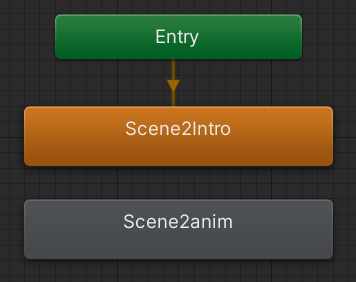
\includegraphics [width=.50\columnwidth, angle=0]
            {Scene2Anim}
	\caption{La struttura dell'animator controller "Scene2IntroController"} 
	\label{4fig:scene2anim}
\end{figure}

Come già anticipato nei capitoli precedenti, una volta che il prodotto vitivinicolo è stato riconosciuto l'applicazione carica la scena dedicata alla selezione dell'annata del vino. Il controller all'avvio della nuova scena, è nello stato \textit{Entry} che attiva, tramite una transizione, l'animazione \textit{Scene2Intro} che si occupa si effettuare lo scorrimento della finestra dal basso verso l'altro fino a metà schermo per permettere all'utente di poter scegliere l'annata della bottiglia di vino di suo interesse.

Dopo aver scelto l'annata, l'utente preme il bottone "Avanti" che attiva la scena \textit{Scene2anim} che effettua lo scorrimento completo della finestra per creare un effetto di transizione verso l'ultima scena dell'applicazione che mostra le tre sezioni "Osserva", "Ascolta" e "Racconta".


\section{Il database MongoDB}

Il database MongoDB, come già accennato, contiene i dati relativi ai vigneti monitorati dall'azienda Trace Technologies. Ogni documento MongoDB contiene i dati di un vigneto strutturati in figura \ref{4fig:mongodb1} dove:

\begin{figure}[h]
	\centering
	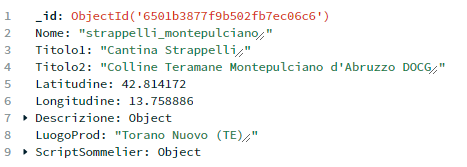
\includegraphics [width=.95\columnwidth, angle=0]
            {mongodb1}
	\caption{Documento MongoDB della cantina Strappelli}
	\label{4fig:mongodb1}
\end{figure}

\begin{itemize}
    \item \textit{Nome}: rappresenta il nome univoco del prodotto vitivinicolo;
    \item \textit{Titolo1}: contiene il nome che appare nelle intestazioni del prodotto vitivinicolo nelle varie sezioni dell'applicazione Android;
    \item \textit{Titolo2}: contiene le sotto-intestazioni del prodotto vitivinicolo nelle varie sezioni dell'applicazione Android;
    \item \textit{Latitudine}: memorizza la latitudine del campo associato al vigneto;
    \item \textit{Longitudine}: memorizza la longitudine del campo associato al vigneto;
    \item \textit{Descrizione}: contiene una breve descrizione delle caratteristiche del vino associato alla bottiglia riconosciuta suddivisa per annata;
    \item \textit{LuogoProd}: contiene il luogo in cui il vino viene prodotto;
    \item \textit{ScriptSommelier}: memorizza un dizionario per ogni annata in cui ad ogni timestamp in secondi è associata una stringa di testo. Questo campo viene utilizzato nella sezione "Ascolta" descritta in precedenza per ottenere il testo sincronizzato con l'audio (figura \ref{4fig:mongodb2}).
\end{itemize}


\begin{figure}[h]
	\centering
	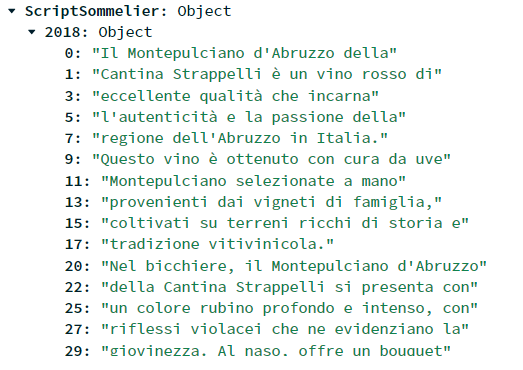
\includegraphics [width=.65\columnwidth, angle=0]
            {mongodb2}
	\caption{Struttura del campo "ScriptSommelier"}
	\label{4fig:mongodb2}
\end{figure}

%\part{Impatto ambientale}
\chapter{Implementazione e manuale utente}
\chapter{Confronto con sistemi di tracciamento}
\chapter{Discussione in merito al lavoro svolto}

\begin{preamble}
{\em
Questo capitolo sarà incentrato sull'analisi del lavoro dedicato alla creazione dell'applicazione Android. In particolare, saranno esaminate le differenze e le similitudini con l'applicazione Vivino, attualmente molto popolare tra gli utenti, al fine di mettere in evidenza le potenzialità dell'applicazione mobile oggetto della tesi. \newline \indent Successivamente, verrà condotta un'approfondita analisi SWOT per evidenziare i punti di forza, di debolezza, le opportunità e le minacce della nostra applicazione.
}
\end{preamble}

\section{Confronto con l'app Vivino}

Vivino (Figura \ref{7fig:logoVivino}) è una popolare app mobile e una piattaforma online che si concentra sulla degustazione e sulla condivisione di recensioni e informazioni sul vino. Gli utenti di Vivino possono utilizzare l'app per scansionare etichette di bottiglie di vino e ottenerne informazioni dettagliate, come recensioni, punteggi, descrizioni, abbinamenti cibo-vino e prezzi. Inoltre, gli utenti possono anche recensire i vini, tenere traccia dei loro preferiti e connettersi con altri amanti del vino sulla piattaforma.

Vivino è diventato uno strumento popolare per gli appassionati di vino che desiderano esplorare e scoprire nuovi prodotti, condividere le proprie esperienze e prendere decisioni informate sugli acquisti. La piattaforma contiene una vasta quantità di dati sul vino e gestisce una comunità di appassionati del settore in cui è possibile condividere opinioni e consigli.

L'applicazione oggetto della presente tesi condivide molti aspetti in comune con l'applicazione Vivino, poiché entrambi sfruttano il riconoscimento delle bottiglie di vino attraverso l'utilizzo della fotocamera. Tuttavia, le differenze risiedono negli obiettivi in quanto Vivino si concentra sulla creazione di una community di appassionati del vino che condividono recensioni e descrizioni sui prodotti vitivinicoli. D'altra parte, l'applicazione oggetto della tesi combina le informazioni di base sul vino con lo stato di salute del vigneto di provenienza, utilizzando sia i dati satellitari che quelli provenienti dalla stazione IoT.

\begin{figure}[h]
	\centering
	
\includegraphics [width=.45\columnwidth, angle=0]
            {logoVivino}
	\caption{Logo dell'applicazione Vivino}
	\label{7fig:logoVivino}
\end{figure}

\section{SWOT Analysis del progetto}

L'analisi SWOT (\textit{Strengths}, \textit{Weaknesses}, \textit{Opportunities}, \textit{Threats}) è uno strumento di pianificazione e valutazione utilizzato nelle aziende, nelle organizzazioni, e persino dalle singole persone. Consiste nell'identificazione e nell'analisi dei punti di forza, di debolezza, delle opportunità e delle minacce rilevanti in una determinata situazione o contesto. I fattori chiave dell'analisi SWOT sono:

\begin{itemize}

	\item Punti di forza \textit{(Strengths)}: identifica i punti di forza interni che possono mitigare i rischi.
	
	\item Debolezze \textit{(Weaknesses)}: identifica le debolezze interne che possono aumentare i rischi.

	\item Opportunità \textit{(Opportunities)}: identifica le opportunità esterne che possono ridurre i rischi o fornire alternative.
	
	\item Minacce \textit{(Threats)}: identifica le minacce esterne che possono aumentare i rischi.

\end{itemize}

Per condurre una \textit{SWOT analysis} è importante identificare con precisione questi fattori, sia interni che esterni. Gli elementi interni sono sotto il controllo dell'organizzazione e possono essere influenzati direttamente, mentre gli elementi esterni sono fuori dal controllo dell'organizzazione, ma possono comunque avere un impatto significativo sulla strategia.

Una \textit{SWOT analysis} aiuta ad identificare il modo in cui sfruttare i punti di forza e le opportunità, mitigare i punti deboli e affrontare le minacce. Questa analisi fornisce una base solida per la pianificazione strategica e la presa di decisioni aziendali informate.

Per condurre la \textit{SWOT Analysis}, è importante definire il concetto di \textit{Smoke Test}. Lo \textit{Smoke Test} rappresenta una metodologia essenziale per la validazione di un'idea di business, garantendo che il prodotto o servizio proposto sia realmente in linea con le aspettative dei futuri clienti. Lo scopo principale di questo test è determinare se i potenziali clienti manifestano un interesse reale per l'offerta. La chiave del successo è far percepire loro che il prodotto o servizio è già disponibile sul mercato. Questo processo è cruciale per validare l'idea e coinvolgere potenziali clienti ancor prima del lancio ufficiale del prodotto.

La \textit{SWOT Analysis} dell'applicazione è riportata di seguito.

\begin{itemize}
	\item Strenghts:
	\begin{itemize}
		\item L'applicazione fornisce in tempo reale informazioni sullo stato di salute del vigneto, facilitando il lavoro degli operatori agricoli nella gestione dei terreni coltivati. Gli utenti possono ottenere dettagli sul vino di interesse, aumentando la loro consapevolezza riguardo al prodotto vinicolo che stanno acquistando.
		\item L'azienda potrebbe ampliare le proprie operazioni estendendo l'analisi dei dati non solo al vino, ma anche ad altri prodotti vitivinicoli. Questo approccio potrebbe incrementare le opportunità di diffusione dell'applicazione.
		\item L'applicazione risulta molto intuitiva nell'utilizzo e questo migliora notevolmente il tempo di permanenza dell'utente e il suo grado di soddisfazione durante l'utilizzo dell'app.
		\item L'applicazione è totalmente gratuita per gli utenti, massimizzandone le probabilità di diffusione.	
	\end{itemize}
	\item Weaknesses:
	\begin{itemize}
		\item Il team di sviluppo software dovrà essere ampliato in seguito all'introduzione di nuove feature, aumentando, così, il costo di sviluppo dell'applicazione.
		\item Allo stato attuale, l'applicazione non è scaricabile dalla piattaforma \textit{Google Play Store}. Questo aspetto può aumentare le difficoltà nell'eseguire lo \textit{Smoke Test}.
	\end{itemize}
	\item Opportunities:
	\begin{itemize}
		\item L'azienda \textit{Trace Technologies} mantiene un costante dialogo con le aziende vitivinicole tramite il servizio "Vigneto Sicuro", raccogliendo feedback in modo continuo per individuare nuove esigenze nel settore agricolo. Inoltre, l'azienda si impegna a soddisfare tali necessità attraverso l'efficiente utilizzo dei dati in agricoltura, integrando le soluzioni richieste direttamente nell'applicazione.
		\item L'applicazione è in costante evoluzione e può adattarsi rapidamente alle esigenze degli utenti, identificate attraverso lo \textit{Smoke Test}. Questo permette di migliorare rapidamente la diffusione dell'applicazione, garantendo un allineamento tempestivo con le richieste degli utenti.	
		\item I settori in cui l'applicazione è inserita abbracciano due ambiti fortemente in crescita, come l'analisi dei dati e la viticoltura.
	\end{itemize}
	\item Threats:
	\begin{itemize}
		\item Lo \textit{Smoke Test} potrebbe rivelare nuove funzionalità non previste ma molto richieste dagli utenti, generando un aumento dell'impegno da parte degli sviluppatori e, di conseguenza, un aumento dei costi nello sviluppo dell'applicazione.
		\item Gli utenti mostrano una bassa retention durante l'utilizzo dell'applicazione, probabilmente a causa di un'esperienza utente non sufficientemente coinvolgente o di informazioni presenti che non risultano di interesse per l'utilizzatore finale.
	\end{itemize}
\end{itemize}
%\part{Linee guida}
\chapter{Conclusioni}

Il lavoro svolto nella tesi si è concentrato sullo sviluppo del prototipo di un'applicazione Android in grado di riconoscere le bottiglie di vino al fine di visualizzare informazioni relative allo stato di salute del vigneto di provenienza. Inizialmente, sono stati identificati gli strumenti software necessari per l'implementazione dell'applicazione Android, come \textit{Unity}, \textit{Vuforia Engine}, e \textit{Polycam}. Successivamente, sono stati definiti nel dettaglio gli aspetti progettuali del lavoro. Dopo la selezione degli strumenti, sono state scelte le versioni di ciascun software per evitare problemi di compatibilità, seguite dall'illustrazione dettagliata dei Class Diagram e Sequence Diagram per ottenere una visione più chiara degli aspetti software cruciali dell'applicazione.

Successivamente, sono state presentate e descritte approfonditamente le classi C\# rilevanti del progetto per chiarire ogni aspetto implementativo dell'applicazione e giustificare le scelte progettuali effettuate durante la progettazione.

L'ultima parte del lavoro si è concentrata sul confronto dell'applicazione con i sistemi di tracciamento dei prodotti alimentari, con l'obiettivo di analizzare i punti in comune e le differenze tra l'applicazione e questi sistemi.

Successivamente, è stata condotta una discussione sui rischi identificati nel progetto, fornendo un'accurata SWOT Analysis. Infine, sono stati indicati i possibili sviluppi futuri del prototipo dell'applicazione mobile.

Di seguito, verranno illustrati i possibili sviluppi futuri dell'applicazione al fine di evidenziarne le potenzialità:

\begin{enumerate}
	\item in futuro, potrebbe essere implementato un sistema per fornire ed elaborare dati rilevanti alle autorità sanitarie nel momento in cui è necessaria una campagna di richiamo di un lotto pericoloso nel settore vitivinicolo.
	\item un'altra possibile evoluzione dell'applicazione potrebbe coinvolgere l'integrazione della piattaforma web proprietaria di Trace Technologies, denominata "Vigneto Sicuro", all'interno dell'applicazione. Ciò consentirebbe agli utenti registrati e agli operatori del settore di accedere a ulteriori dati su specifici prodotti vitivinicoli.
	\item potrebbe essere considerata la creazione di una piattaforma per la condivisione delle recensioni da parte dei sommelier. Questi esperti potrebbero condividere le informazioni sui vini registrati all'interno della piattaforma fornita da Trace Technologies, incoraggiando le aziende agricole a sottoscrivere l'abbonamento alla piattaforma "Vigneto Sicuro".
\end{enumerate}


% APPENDICES
%\appendix
%\include{appendix1/appendix1}
%\include{appendix2/appendix2}

%% BACKMATTER %%
% The pages inside of backmatter are in Arabic numerals and the chapters will not have numeration
\backmatter

% BIBLIOGRAPHY WITH BIBTEX %
%*******************************************************
% Bibliography
%*******************************************************
\cleardoublepage
\phantomsection
\addcontentsline{toc}{chapter}{\bibname}
\nocite{*}
% The style can be: classic, plainnat, abbrvnat or unsrtnat
\bibliographystyle{classic}
\bibliography{bibliography}
%

\vspace{2.5cm}
\begin{Large}Siti web consultati\end{Large}
\begin{itemize}
    \item Unity Real-Time Development Platform | 3D, 2D, VR \& AR Engine -- \url{www.unity.com};
    \item Vuforia Engine Developer Portal \url{https://developer.vuforia.com};
    \item Polycam - LiDAR \& 3D Scanner for iPhone \& Android \url{https://poly.cam};
    \item blender.org - Home of the Blender project - Free and Open 3D Creation Software \url{https://www.blender.org};
    \item Google Earth Studio \url{https://www.google.com/intl/it/earth/studio/};
    \item MongoDB: La Piattaforma Di Dati Applicativi | MongoDB \url{https://www.mongodb.com/it-it};
\end{itemize}


% All the sources are described in a file named bibliography.bib
% if you want to cite one in the text:
% \citep{label}
% In order to update the bibliography you have to execute:
% bibtex main (without ".tex")

\chapter*{Ringraziamenti}
\addcontentsline{toc}{chapter}{Ringraziamenti}
\markboth{Ringraziamenti}
\emph{

} 

% INDEX %
%\cleardoublepage
% To help hyperref to jump to the correct page
\phantomsection
% To add the Index in the table of contents
\addcontentsline{toc}{chapter}{Indice analitico}
% Prints the Index
\printindex
% To add an item in it, write the \index{WORD} after the word to highlight:
% WORD\index{WORD}
% In order to update the Index you have to execute:
% makeindex main (without ".tex")

% A typical session involving a bibliography, an index and son on would require:
% pdflatex main
% makeindex -s main.ist -t main.alg -o main.acr main.acn
% makeindex -s main.ist -t main.glg -o main.gls main.glo
% bibtex main
% pdflatex main
% pdflatex main
% makeindex main
% makeindex -s main.ist -t main.alg -o main.acr main.acn
% makeindex -s main.ist -t main.glg -o main.gls main.glo
% pdflatex main
% pdflatex main
\end{document}